%%%%%%%%%%%%%%%%%%%%%%%%%%%%%%%%%%%%%%%%%%%%%%%%%%%%%%%%%%%%%%%
%% OXFORD THESIS TEMPLATE

% Originally by Keith A. Gillow (gillow@maths.ox.ac.uk), 1997
% Modified by Sam Evans (sam@samuelevansresearch.org), 2007
% Modified by John McManigle (john@oxfordechoes.com), 2015
% Modified by Maud Gautier (https://github.com/MaudGautier), 2019
% Modified by Thibault Latrille (https://github.com/ThibaultLatrille), 2020
%
% This version Copyright (c) 2020 Thibault Latrille
%
% Broad permissions are granted to use, modify, and distribute this software
% as specified in the MIT License included in this distribution's LICENSE file.

%%%%% CHOOSE PAGE LAYOUT
%\documentclass[a4paper,openright,twoside]{thesis}
\documentclass[a4paper,oneside,nobind]{thesis}

% Caption
\usepackage[font=footnotesize,labelfont=bf]{caption}
\usepackage{float}
\usepackage{tabularx}
\makeatletter
\newcommand\cellwidth{\TX@col@width}
%\floatstyle{boxed} 
%\restylefloat{figure}
%\usepackage{floatpag}

% To add blank lines
\usepackage{parselines} 
% To add a blank figure
\usepackage{todonotes}

% To keep old font size even if not the case in cover page
\makeatletter
\newcommand{\savefont}{\xdef\oldfontsize{\f@size}\xdef\oldblskip{\f@baselineskip}}
\newcommand{\backtoppevfont}{\fontsize{\oldfontsize}{\oldblskip}\selectfont}
\makeatother

% spacing lines
\usepackage{hhline}
\usepackage{multirow}
\setlength{\arrayrulewidth}{1.4pt}
\usepackage{setspace}
\newcommand{\tocless}[2]{\bgroup\let\addcontentsline=\nocontentsline#1{#2}\egroup}

%%%%% SELECT YOUR DRAFT OPTIONS
% Three options going on here; use in any combination.  But remember to turn the first two off before
% generating a PDF to send to the printer!

% This adds a "DRAFT" footer to every normal page.  (The first page of each chapter is not a "normal" page.)
% \fancyfoot[C]{\color{PURPLEDARKsection} \emph{DRAFT Printed on \today}}

% This highlights (in blue) corrections marked with (for words) \mccorrect{blah} or (for whole
% paragraphs) \begin{mccorrection} . . . \end{mccorrection}.  This can be useful for sending a PDF of
% your corrected thesis to your examiners for review.  Turn it off, and the blue disappears.
% \correctionstrue

% Define colors
\usepackage{xcolor, colortbl}
\definecolor{RED}{HTML}{EB6231}
\definecolor{YELLOW}{HTML}{E29D26}
\definecolor{BLUE}{HTML}{5D80B4}
\definecolor{LIGHTGREEN}{HTML}{6ABD9B}
\definecolor{GREEN}{HTML}{8FB03E}
\definecolor{PURPLE}{HTML}{BE1E2D}
\definecolor{BROWN}{HTML}{A97C50}
\definecolor{PINK}{HTML}{DA1C5C}
\definecolor{PURPLEDARK}{cmyk}{0, 0.5, 0, 0.7}
\definecolor{PURPLELIGHT}{cmyk}{0, 0.12, 0, 0.2}
\definecolor{PURPLEGREY}{cmyk}{0, 0.5, 0, 0.55}
\definecolor{GREYDARK}{cmyk}{0, 0, 0, 0.92}
\definecolor{BLUELINK}{HTML}{0645AD}
\definecolor{DARKBLUELINK}{HTML}{0B0080}
\definecolor{LIGHTBLUELINK}{HTML}{3366BB}
\definecolor{PURPLELINK}{HTML}{663366}

\definecolor{Nonpolar}{HTML}{E29D26}
\definecolor{Acidic}{HTML}{EB6231}
\definecolor{Basic}{HTML}{5D80B4}
\definecolor{Polar}{HTML}{6ABD9B}
\definecolor{Stop}{HTML}{6ABD9B}


%%%%% BIBLIOGRAPHY SETUP
\usepackage{natbib} % add [numbers] if I want to count them
\newcommand*{\bibtitle}{References}
\pdfinclusioncopyfonts=1

% Uncomment this if you want equation numbers per section (2.3.12), instead of per chapter (2.18):
%\numberwithin{equation}{subsection}

% refs and backref
\usepackage{usebib}
\usepackage{backref}
\usepackage{hyperref}
\hypersetup{colorlinks,
	linkcolor=GREYDARK,
	citecolor=DARKBLUELINK,
	urlcolor=BLUELINK
} % Color citation links in purple
\renewcommand*{\backrefsep}{,~}%
\renewcommand*{\backreftwosep}{,~}% ', and~'
\renewcommand*{\backreflastsep}{,~}% ' and~'

% Deal with backreferences in bibliography
\newcommand{\mapolicebackref}[1]{\hspace*{\fill} \mbox{\textit {\small #1}}}
\renewcommand*{\backref}[1]{}
\renewcommand*{\backrefalt}[4]{%
\ifcase #1 \mapolicebackref{Not cited}
\or \mapolicebackref{Cited at page #2}
    \else \mapolicebackref{Cited at pages #2}
\fi
}
%\bibinput{references}
% Misc
\usepackage{amsfonts,amsmath,mathtools}
\usepackage{bm}
\usepackage{listings, enumerate, enumitem}
\usepackage{pgfplots, pgf, tikz}
\usetikzlibrary{arrows,automata,calc}
\pgfplotsset{every axis/.append style={line width=1pt}}
\pgfplotscreateplotcyclelist{colors}{RED\\YELLOW\\BLUE\\LIGHTGREEN\\GREEN\\}
\usepackage{titlesec}
\usepackage[toc, acronym]{glossaries}
\makeglossaries
\definecolor{RED}{HTML}{EB6231}
\definecolor{YELLOW}{HTML}{E29D26}
\definecolor{BLUE}{HTML}{5D80B4}
\definecolor{LIGHTGREEN}{HTML}{6ABD9B}
\definecolor{GREEN}{HTML}{8FB03E}
\definecolor{PURPLE}{HTML}{BE1E2D}
\definecolor{BROWN}{HTML}{A97C50}
\definecolor{PINK}{HTML}{DA1C5C}

\newcommand{\specialcell}[2][c]{%
	\begin{tabular}[#1]{@{}c@{}}#2\end{tabular}}

\DeclareMathOperator{\E}{\mathbb{E}}
\newcommand{\der}{\mathrm{d}}
\newcommand{\angstrom}{\text{\normalfont\AA}}
\newcommand{\e}{\mathrm{e}}
\newcommand{\dnds}{d_N / d_S}
\newcommand{\indice}{l}
\newcommand{\indiceexp}{^{(\indice)}}
% Time, effective population size and mutation rate.
\newcommand{\Ne}{N_{\textrm{e}}}
% \acrshort{DNA}
\newcommand{\SetNuc}{\Omega_{\mathrm{N}}}
\newcommand{\SetWeak}{\Omega_{\mathrm{W}}}
\newcommand{\SetStrong}{\Omega_{\mathrm{S}}}
\newcommand{\mutmatrix}{R}
\newcommand{\Mutmatrix}{\bm{\mutmatrix}}
\newcommand{\exchan}{\rho}
\newcommand{\Exchan}{\bm{\exchan}}
\newcommand{\mutequi}{\sigma}
\newcommand{\Mutequi}{\bm{\mutequi}}
% Codons
\newcommand{\SetCodon}{\Omega_{\mathrm{C}}}
\newcommand{\ci}{{i}}
\newcommand{\cj}{{j}}
\newcommand{\iSetCodon}{1 \leq \ci \leq 61}
\newcommand{\jSetCodon}{1 \leq \cj \leq 61}
\newcommand{\ijSetCodon}{1 \leq \ci, \cj \leq 61}
\newcommand{\itoj}{\ci, \cj}
\newcommand{\jtoi}{\cj, \ci}
\newcommand{\nucitoj}{\mathcal{M}(\itoj)}
\newcommand{\submatrix}{Q}
\newcommand{\Submatrix}{\bm{\submatrix}}
\newcommand{\subequi}{\pi}
\newcommand{\Subequi}{\bm{\subequi}}
\newcommand{\probmatrix}{P}
\newcommand{\Probmatrix}{\bm{\probmatrix}}
% Amino-acids
\newcommand{\aminoacid}{\text{A}}
\newcommand{\aSetAa}{1 \leq \aminoacid \leq 20}
\newcommand{\SetAa}{\Omega_{\mathrm{A}}}
\newcommand{\Neighbor}{\mathcal{V}}
\newcommand{\NonSyn}{\mathcal{N}}
\newcommand{\Syn}{\mathcal{S}}
\newcommand{\Nx}{\Neighbor_x}
\newcommand{\NxAB}{\Neighbor_x^{\mathrm{A} \rightarrow \mathrm{B}}}
\newcommand{\NyBA}{\Neighbor_x^{\mathrm{B} \rightarrow \mathrm{A}}}
\newcommand{\NxWS}{\Neighbor_x^{\mathrm{W} \rightarrow \mathrm{S}}}
\newcommand{\NxSS}{\Neighbor_x^{\mathrm{S} \rightarrow \mathrm{S}}}
\newcommand{\NxSW}{\Neighbor_x^{\mathrm{S} \rightarrow \mathrm{W}}}
\newcommand{\NxWW}{\Neighbor_x^{\mathrm{W} \rightarrow \mathrm{W}}}
\newcommand{\NyWS}{\Neighbor_y^{\mathrm{W} \rightarrow \mathrm{S}}}
\newcommand{\NySS}{\Neighbor_y^{\mathrm{S} \rightarrow \mathrm{S}}}
\newcommand{\NySW}{\Neighbor_y^{\mathrm{S} \rightarrow \mathrm{W}}}
\newcommand{\NyWW}{\Neighbor_y^{\mathrm{W} \rightarrow \mathrm{W}}}
\newcommand{\NxNonSyn}{\NonSyn_x}
\newcommand{\NyNonSyn}{\NonSyn_y}
\newcommand{\NxSyn}{\Syn_x}
\newcommand{\NySyn}{\Syn_y}
\newcommand{\aai}{\mathcal{A}(\ci)}
\newcommand{\aaj}{\mathcal{A}(\cj)}
\newcommand{\Ni}{\mathcal{N}_{\mathrm{eighbors}}\left(\ci\right)}
\newcommand{\NiNonSyn}{\mathcal{N}_{\mathrm{onSyn}}\left(\ci\right)}
\newcommand{\NiSyn}{\mathcal{S}_{\mathrm{yn}}\left(\ci\right)}
\newcommand{\fit}{f}
\newcommand{\Fit}{\bm{\fit}}
\newcommand{\fiti}{\fit_{\aai}}
\newcommand{\fitj}{\fit_{\aaj}}
\newcommand{\Fiti}{F_{\aai}}
\newcommand{\Fitj}{F_{\aaj}}
\newcommand{\scaledfit}{F}
\newcommand{\ScaledFit}{\bm{\scaledfit}}
\newcommand{\scaledfiti}{\scaledfit_{\aai}}
\newcommand{\scaledfitj}{\scaledfit_{\aaj}}
\newcommand{\selcoef}{{\delta_{\fit}}}
\newcommand{\scaledselcoef}{{\Delta \scaledfit}}
% Categories
\newcommand{\Seqitoj}{\ci, \cj}
\newcommand{\setNeighbors}{\mathcal{M}\left(\ci\right)}
\newcommand{\setNonSynNeighbors}{\mathcal{N}\left(\ci\right)}
\newcommand{\setSynNeighbors}{\mathcal{S}\left(\ci\right)}

% make part like a chapter
\titleclass{\part}{top} 
\titleformat{\part}
[display]
{\centering\fontsize{36}{0}}
{\color{GREYDARK} \bfseries \centering \fontsize{36}{0}{\partname} \thepart}
{36pt}
{\color{GREYDARK} \bfseries \centering \fontsize{36}{0}}[\titlepagedecoration]

% Epigraphs
\usepackage{epigraph}
\renewcommand\epigraphflush{flushright}
\renewcommand\epigraphsize{\normalsize}
\setlength\epigraphwidth{0.7\textwidth}

\DeclareFixedFont{\titlefont}{T1}{ppl}{b}{it}{0.5in}

%%%%% PAGE DECORATION AND FORMATTING

% Decorate title pages (for parts)
\newcommand\titlepagedecoration{%
\thispagestyle{empty}
\begin{tikzpicture}[remember picture,overlay,shorten >= -10pt]

\coordinate (aux1) at ([yshift=-15pt]current page.north east);
\coordinate (aux2) at ([yshift=-410pt]current page.north east);
\coordinate (aux3) at ([xshift=-4.5cm]current page.north east);
\coordinate (aux4) at ([yshift=-150pt]current page.north east);

\begin{scope}[opacity=0.75,BLUE,line width=12pt,rounded corners=12pt]
\draw
  (aux1) -- coordinate (a)
  ++(225:5) --
  ++(-45:5.1) coordinate (b);
\draw[shorten <= -10pt]
  (aux3) --
  (a) --
  (aux1);
\draw[opacity=0.5,YELLOW,shorten <= -10pt]
  (b) --
  ++(225:2.2) --
  ++(-45:2.2);
\end{scope}
\draw[opacity=0.75,RED,line width=8pt,rounded corners=8pt,shorten <= -10pt]
  (aux4) --
  ++(225:0.8) --
  ++(-45:0.8);
\begin{scope}[opacity=0.75,LIGHTGREEN,line width=6pt,rounded corners=8pt]
\draw[shorten <= -10pt]
  (aux2) --
  ++(225:3) coordinate[pos=0.45] (c) --
  ++(-45:3.1);
\draw
  (aux2) --
  (c) --
  ++(135:2.5) --
  ++(45:2.5) --
  ++(-45:2.5) coordinate[pos=0.3] (d);   
\draw 
  (d) -- +(45:1);
\end{scope}
\end{tikzpicture}%
}
% Modify chapter color
\colorlet{chaptergrey}{PURPLELIGHT}
\renewcommand*\sectfont{\bfseries\color{PURPLEDARK}}

% Format titles
\titleformat{\section}
{\color{GREYDARK}\normalfont\Large\bfseries}
{\color{GREYDARK}\thesection}{1em}{}

\titleformat{\subsection}
{\color{GREYDARK}\normalfont\large\bfseries}
{\color{GREYDARK}\thesubsection}{1em}{}

\titleformat{\subsubsection}
{\color{GREYDARK}\normalfont\bfseries}
{\color{GREYDARK}\thesubsubsection}{1em}{}

% Titles for toc
\usepackage{titletoc}
\usepackage{minitoc}

% If uncommented, then rules in tables are in purple
% \makeatletter
% \arrayrulecolor{PURPLEDARKsection}
% \def\mtc@bottom@rule{%
%   \ifx\mtc@rule\relax\relax\else
%       \vskip -2.5ex
%         \color{PURPLEDARKsection}\rule[2.4\p@]{\columnwidth}{.4\p@}\vspace*{2.6\p@}\fi}
% \makeatother
%
\renewcommand*\rhead{\textcolor{RED}}
% Change appendix title page (+ some modif in ociamthesis.cls to remove from toc + added in toc via adding doubleclearpage and phantomsection and line toc when calling \startappendices — see below)
\makeatletter
\renewcommand{\@chap@pppage}{}
\makeatother

%%%%% ADD YOUR PERSONAL MACROS
% To make text superscripts shortcuts
\renewcommand{\th}{\textsuperscript{th}}
\newcommand{\nd}{\textsuperscript{nd}}
\renewcommand{\st}{\textsuperscript{st}}
\newcommand{\rd}{\textsuperscript{rd}}

%%%%% THE ACTUAL DOCUMENT STARTS HERE
\begin{document}
\thispagestyle{empty}
\vspace*{\stretch{1}}

\unitlength 1cm
\begin{center}

    \vspace*{-2.5cm}
    \begin{figure}[h]
        \centering
        
\includegraphics[width=0.8\textwidth]{figures/logo-UdL-UCB}
    \end{figure}

    {\large \textbf{THÈSE de DOCTORAT DE L'UNIVERSITÉ DE LYON}\\}
    {Opérée au sein de~:\\}
    {\large \textbf{l'Université Claude Bernard Lyon 1}\\}
    \vspace{12pt}
    {\large \textbf{Ecole Doctorale} 341 \\
    \vspace{0.15cm}
    Écosystèmes Évolution Modélisation Microbiologie
    }
    
    \vspace{12pt}

    {\large \textbf{Spécialité de doctorat~:} Génomique évolutive
    \\}

    \vspace{0.8cm}

    %{Soutenue publiquement le jj/mm/aaaa, par~:\\}
    {Soutenance prévue le 30/11/2020, par~:\\}
    \vspace{0.15cm}
    {\Large \textbf{Thibault Latrille}}
    \vspace{0.5cm}

    \rule{5cm}{1pt}
    \vspace{12pt}

    {\huge \textbf{Modélisation de l'articulation des mécanismes sélectifs et neutres dans l’évolution des séquences d’ADN codant pour des protéines.}\par}

    \vspace{12pt}
    \rule{5cm}{1pt}

    \vspace{0.5cm}

\end{center}

Devant le jury composé de~:\\

\small {
\begin{tabular}{ll}
    \textbf{Celine BROCHIER-ARMANET} & \textbf{Présidente}         \\
    Professeure, Université Claude Bernard Lyon 1 \\
    \textbf{Julien Yann DUTHEIL}     & \textbf{Rapporteur}         \\
    Research Group Leader, Max Planck Institute (Allemagne) \\
    \textbf{Richard GOLDSTEIN}       & \textbf{Rapporteur}         \\
    Professeur, University College London (Royaume-Uni) \\
    \textbf{Carina Farah MUGAL}      & \textbf{Rapporteure}        \\
    Chercheure, Uppsala University (Suède) \\
    \textbf{Nicolas LARTILLOT}       & \textbf{Directeur de thèse} \\
    Directeur de recherche, CNRS/LBBE \\
\end{tabular}
}
\vspace*{\stretch{3}}
%%%%% CHOOSE YOUR LINE SPACING HERE
\setlength{\textbaselineskip}{1.2em}
% You can set the spacing here for the roman-numbered pages (acknowledgements, table of contents, etc.)
\setlength{\frontmatterbaselineskip}{1.2em}
% Leave this line alone; it gets things started for the real document.
\setlength{\baselineskip}{\textbaselineskip}

%%%%% CHOOSE YOUR SECTION NUMBERING DEPTH HERE
% The level that gets a number:
\setcounter{secnumdepth}{2}
% The level that shows up in the ToC:
\setcounter{tocdepth}{2}

%%%%% DEDICATION
\begin{dedication}
	\thispagestyle{empty}
	\begin{center}
		\includegraphics[width=\textwidth, page=1] {figures/preface.pdf}
	\end{center} 
\end{dedication}

%%%% EPIGRAPH
\begin{alwayssingle}
	\thispagestyle{empty}
	\vspace*{\fill}
	\makebox[\textwidth][r] {
		\begin{minipage}[t]{8cm}
			\emph{}\\
			\hfill \slshape{L'humanité est constamment aux prises avec deux processus contradictoires dont l'un tend à instaurer l'unification, tandis que l'autre vise à maintenir ou à rétablir la diversification.}\\
			\hfill \qauthor{Claude Lévi-Strauss.}
		\end{minipage}
	}

	\vspace*{\fill}
	\vspace*{\fill} 
\end{alwayssingle}


% %%%%% ABSTRACT SEPARATE
% % This is used to create the separate, one-page abstract that you are required to hand into the Exam
% % Schools.  You can comment it out to generate a PDF for printing or whatnot.
% \begin{abstractseparate}
%     \thispagestyle{empty}
\vspace*{\stretch{1}}


\begin{center}
	\LARGE \textbf{Modeling the articulation of adaptive and neutral mechanisms in the evolution of protein coding DNA sequences}
\end{center}

\section*{Abstract}
Selection in protein-coding sequences can be detected based on multiple sequence alignments using phylogenetic codon models.
Mechanistic approaches, grounded on population-genetics first principles, explicitly formalize the interplay between mutation, selection and random drift, and return an estimate of the amino-acid fitness landscape.
However, these recently developed models rely on the assumption of constant effective population size.
We propose an extended mutation-selection model reconstructing site-dependent fitness landscape, long-term trends in effective population size and mutation rate along the phylogeny, from an alignment of DNA coding sequences.
Independently, ancestral life-history traits are reconstructed along the phylogeny from observation in present-day species.
Together, we estimate the correlation between reconstructed life-history traits, mutation rate and effective population size, intrinsically including phylogenetic inertia.
Our framework has been tested against simulated data, and in empirical data in mammals and primates.
Finally, our work also points to important theoretical questions about how coding sequences respond to changes in effective population size and to fluctuating selection.\\

\textbf{keywords: }{Phylogenetic, codon models, mutation-selection models, population genetic, population size, mutation rate, life history traits.}

\vspace*{\stretch{3}}
\newpage % Create an abstract.tex file in the 'text' folder for your abstract.
% \end{abstractseparate}
%
% \newgeometry{inner=2cm, outer=2cm, top=2cm, bottom=2cm}
\begin{alwayssingle}
\begingroup
	\pagenumbering{gobble}% Turn off page numbering for abstract and acknowlegements
\thispagestyle{empty}
\vspace*{\stretch{1}}


\begin{center}
	\LARGE \textbf{Modeling the articulation of adaptive and neutral mechanisms in the evolution of protein coding DNA sequences}
\end{center}

\section*{Abstract}
Selection in protein-coding sequences can be detected based on multiple sequence alignments using phylogenetic codon models.
Mechanistic approaches, grounded on population-genetics first principles, explicitly formalize the interplay between mutation, selection and random drift, and return an estimate of the amino-acid fitness landscape.
However, these recently developed models rely on the assumption of constant effective population size.
We propose an extended mutation-selection model reconstructing site-dependent fitness landscape, long-term trends in effective population size and mutation rate along the phylogeny, from an alignment of DNA coding sequences.
Independently, ancestral life-history traits are reconstructed along the phylogeny from observation in present-day species.
Together, we estimate the correlation between reconstructed life-history traits, mutation rate and effective population size, intrinsically including phylogenetic inertia.
Our framework has been tested against simulated data, and in empirical data in mammals and primates.
Finally, our work also points to important theoretical questions about how coding sequences respond to changes in effective population size and to fluctuating selection.\\

\textbf{keywords: }{Phylogenetic, codon models, mutation-selection models, population genetic, population size, mutation rate, life history traits.}

\vspace*{\stretch{3}}
\newpage
\endgroup
\end{alwayssingle}
% JEM: Pages are roman numbered from here, though page numbers are invisible until ToC.  This is in
% keeping with most typesetting conventions.

%%%%% ACKNOWLEDGEMENTS -- Nothing to do here except comment out if you don't want it.
\thispagestyle{empty}
\vspace*{\stretch{1}}

\section*{Remerciements}

Thanks for all the fish!

\vskip\onelineskip
\begin{flushright}
	\textbf{\theauthor}
	\\
	Villeurbanne,\MONTH\the\year
\end{flushright}

\vspace*{\stretch{3}}

\begin{romanpages}
%%%%% MINI TABLES
\dominitoc % include a mini table of contents
%\dominilof  % include a mini list of figures
%\dominilot  % include a mini list of tables
% This aligns the bottom of the text of each page.  It generally makes things look better.
\flushbottom
% This is where the whole-document ToC appears:
\tableofcontents
\newacronym{AA}{AA}{amino-acid}
\newacronym{A}{A}{Adenine}
\newacronym{HB}{HB}{Halpern \& Bruno}
\newacronym{BGC}{BGC}{biased gene conversion}
\newacronym{CUB}{CUB}{codon usage bias}
\newacronym{C}{C}{Cytosine}
\newacronym{DFE}{DFE}{distribution of fitness effects}
\newacronym{DNA}{DNA}{deoxyribonucleic acid}
\newacronym{G}{G}{Guanine}
\newacronym{GTR}{GTR}{General Time Reversible}
\newacronym{GY}{GY}{Goldman \& Yang}
\newacronym{LHT}{LHT}{life history traits}
\newacronym{MCMC}{MCMC}{Monte Carlo Markov Chain}
\newacronym{MC}{MC}{Markov chain}
\newacronym{MG}{MG}{Muse \& Gaut}
\newacronym{MK}{MK}{McDonald \& Kreitman}
\newacronym{ML}{ML}{maximum likelihood}
\newacronym{Ne}{\ensuremath{\Ne}}{effective population size}
\newacronym{RNA}{RNA}{ribonucleic acid}
\newacronym{S}{S}{strong nucleotide (G or C)}
\newacronym{SFS}{SFS}{site frequency spectrum}
\newacronym{T}{T}{Thymine}
\newacronym{tRNA}{tRNA}{transfer RNA}
\newacronym{W}{W}{weak nucleotide (A or T)}
\newacronym{WS}{WS}{Mutation from a ‘weak’ (W) to ‘strong’ (S) nucleotide}

\newglossaryentry{allele}{name={allele},description={A variant form of a given gene}}
\newglossaryentry{bgc}{name={biased gene conversion},description={Process by which gene conversion is biased towards a given outcome. It occurs when one haplotype has a higher probability of being the donor}}
\newglossaryentry{codon-usage-bias}{name={codon usage bias},description={Unequal frequency of the alternative codons that specify the same amino acid}}
\newglossaryentry{codon}{name={codon},description={Sequence of three nucleotides coding for a given amino acid}}
\newglossaryentry{diploid}{name={diploid},description={Organism (or phase) displaying a ploidy of 2 ($n=2$), i.e.\ two sets of chromosomes (which are paired)}}
\newglossaryentry{effective-population-size}{name={effective population size},description={The number of individuals in a population who contribute to the next generation}}
\newglossaryentry{gBGC}{name={GC-biased gene conversion},description={The process by which the GC-content increases because of biased gene conversion}}
\newglossaryentry{GC}{name={GC-content},description={The percentage of G or C nucleotidic bases in a DNA sequence}}
\newglossaryentry{Gamete}{name={gamete},description={Product of meiosis}}
\newglossaryentry{GeneConv}{name={gene conversion},description={A non-reciprocal recombination process that results in one sequence being converted into the other}}
\newglossaryentry{drift}{name={genetic drift},description={The random fluctuation in allele frequencies due to random sampling of individuals}}
\newglossaryentry{Genetic-distance}{name={genetic distance},description={Distance between DNA markers on a chromosome measured as the amount of crossing-overs between them}}
\newglossaryentry{genetic-interference}{name={genetic interference},description={The fact that the formation of a recombination event can affect that of others in adjacent regions}}
\newglossaryentry{genetic-linkage}{name={genetic linkage},description={Non-independent assortment of genes}}
\newglossaryentry{Genotyping}{name={genotyping},description={The process by which DNA is analyzed to determine which genetic variant (allele) is present for a given marker}}
\newglossaryentry{Haploid}{name={haploid},description={Organism (or phase) displaying a ploidy of 1 ($n=1$), i.e.\ a single set of chromosomes}}
\newglossaryentry{N-ter}{name={N-terminus},description={End of an amino acid chain terminated by a free amine group}}
\newglossaryentry{non-synonymous}{name={non-synonymous substitution},description={transition that modifies the amino acid produced}}
\newglossaryentry{Phenotype}{name={phenotype},description={The composite of observable traits}}
\newglossaryentry{ploidy}{name={ploidy},description={The number of complete sets of chromosomes ($n$) in a cell}}
\newglossaryentry{polymorphic}{name={polymorphic},description={Which presents several forms. Subject to inter-individual variability}}
\newglossaryentry{recombination}{name={recombination},description={Exchange of DNA sequence information}}
\newglossaryentry{synonymous}{name={synonymous substitution},description={substitution that does not modify the amino acid produced}}
\newglossaryentry{transition}{name={transition},description={Mutation between two nucleotidic bases of the same family (purine or pyrimidine), i.e.\ either a A~$\leftrightarrow$~G or a C~$\leftrightarrow$~T mutation}}
\newglossaryentry{transversion}{name={transversion},description={Mutation involving a change of nucleotidic family (from a purine to a pyrimidine or the other way round), i.e.\ either a A~$\leftrightarrow$~C, a A~$\leftrightarrow$~T, a G~$\leftrightarrow$~C or a G~$\leftrightarrow$~T mutation}}
\newglossaryentry{Akaike}{name={Akaike information criterion},description={Measure of the relative quality of a maximum likelihood estimated given the data, penalizing for too many parameters in the model}}
\newglossaryentry{Bayes}{name={Bayes factor},description={Ratio of the posterior probability of two competing hypotheses, usually a null and an alternative. The posterior probability is conditioned on randomly observed data and on the prior distribution of the parameters of the competing hypotheses}}
\newglossaryentry{Codon}{name={codon usage bias},description={Differences in the frequency of occurrence of synonymous codons in protein coding DNA, reflecting a balance between mutational biases and natural selection for translational optimization}}
\newglossaryentry{Dirichlet-process}{name={Dirichlet process},description={Family of stochastic processes whose realizations are probability distributions. In other words, a Dirichlet process is a probability distribution whose range is itself a set of probability distributions. It is often used in Bayesian inference to describe the prior knowledge about the distribution of random variables. Meaning, how likely it is that the random variables are distributed according to one or another particular distribution}}
\newglossaryentry{LRT}{name={Likelihood ratio test},description={Statistical test used to compare the goodness of fit of two models, one of which (the null model) is a special case of the other (the alternative model)}}
\newglossaryentry{likelihood}{name={likelihood},description={Probability of observing the data given the parameters of the statistical model. Note this is a function of solely the parameters of the model, the observed data are fixed}}
\newglossaryentry{MKtest}{name={Mc-Donald Kreitman test},description={Test that compares the amount of variation within a species (polymorphism) to the divergence between species (substitutions) at two types of sites, neutral and selected}}
\newglossaryentry{mcmc}{name={Monte Carlo Markov Chain},description={Class of algorithms for sampling from a probability distribution (usually posterior distribution in Bayesian inference) based on constructing a Markov chain that has the desired distribution of its equilibrium distribution}}
\newglossaryentry{mc}{name={Markov chain},description={Stochastic process with property that the next state of the process depends only on the present state of the process and not on its past}}
\newglossaryentry{ml}{name={maximum likelihood},description={Method of estimating the parameters of a model given the data, by finding the parameter value that maximize the likelihood function}}
\newglossaryentry{mixture}{name={mixture model},description={Probabilistic model for representing the presence of subpopulations within an overall population, without requiring that an observed data set should identify the sub-population to which an individual observation belongs}}
\newglossaryentry{nearly-neutral}{name={nearly-neutral},description={Slightly deleterious or advantageous mutations are effectively neutral when their selection coefficient are lower than one divided by the effective population size}}
\newglossaryentry{neutral}{name={neutral},description={Mutations are nor deleterious neither advantageous, their probability of fixation is one divided by twice the effective population size (for diploids)}}
\newglossaryentry{prior}{name={prior},description={Probability distribution that would express one's beliefs about a parameter of the model before the data is taken into account}}
\newglossaryentry{posterior}{name={posterior},description={Probability distribution of a parameter of the model conditioned on randomly observed data and the prior distribution}}
\newglossaryentry{substitution}{name={substitution},description={Point mutation that appeared in only one individual in the population, and subsequently reached fixation in the population}}

\printglossary[type=\acronymtype]
\mtcaddchapter
\printglossary
\mtcaddchapter
\end{romanpages}

%%%% CHAPTERS
\pagenumbering{arabic} 
\flushbottom
\chapter*{Preamble}
\addcontentsline{toc}{part}{Preamble}
This thesis is submitted in partial fulfillment of the requirements
for the degree of \emph{Philosophiae Doctor} at the Université de Lyon.
The research presented here was conducted at the Laboratoire de Biométrie et Biologie Evolutive (LBBE), under the supervision of research director M. Nicolas Lartillot.
This work was conducted from September 2017 onward during a 3 years grant by ENS de Lyon (Contrat Doctoral Spécifique Normalien).
The thesis is a collection of two papers, and two chapters preceded by an introductory chapter that relates them together and provides background information and motivation for the work.

The diversity of living organisms today is the result of a complex and intricate process, which operates at multiple level.
At the molecular level, the fate of protein depends on its ability to fold but also the enzyme it encounters from its creation up to its degradation. 
Composed of billions of proteins, a cell own fate depends on its own ability to metabolize substrates and copy its \acrshort{DNA}, but also depends on the fate of surrounding cells and the individual on which it belongs.
Moreover, the fate of this individual depends on its own behavior, but also depends on its environment and the population on which it belongs.
Altogether, scientists have dissected this intricate process into its core components, trough molecular biology, enzymology, metabolism, physiology, population-genetic, ecology, and so on. 
Molecular evolution seek to encompass different levels, relating molecular changes to higher level evolutionary process.
In this vain, this work is a modest attempt to reconcile several layers of evolution, mechanistically deriving how observable parameters between population and within population are depends in microscopic molecular and cellular parameters.
Specifically, I seek to draw connections between three different dataset, first molecular parameters of protein function, second is the divergence of \acrshort{DNA} sequences between species, formerly is the diversity of \acrshort{DNA} sequences within species.
Altogether through the framework of population genetic.

\fancyhf{} % clear the header and footers
\pagestyle{fancy}
\renewcommand{\chaptermark}[1]{\markboth{\thechapter. #1}{\thechapter. #1}}
\renewcommand{\sectionmark}[1]{\markright{\thesection. #1}} 
\renewcommand{\headrulewidth}{1pt}
\cfoot{\thepage}
\fancypagestyle{plain}{\fancyhf{}\fancyfoot[C]{\emph{\thepage}}}
\fancyhead[LO]{\emph{\leftmark}} 
\fancyhead[RE]{\emph{\rightmark}} 

\part{Introduction}
\label{part:intro}
\thispagestyle{empty}
\chapter{Molecular evolution}
\minitoc
\label{sec:intro}

From the discovery of evolution to today knowledge, the understanding of the mechanisms from which the diversity of life and complexity emerges has seen dramatic changes, and revolution.
One such revolution is called molecular evolution, a recent scientific fields, emerging at the crossroad of evolutionary biology which had seen tremendous theoretical development in the nineteenth and twentieth century, and molecular biology  which recruited advances in chemistry and had seen many technical revolutions.
Molecular evolution borrows strength from the amount of empirical data available from molecular biology, and the predictive power of evolutionary biology.
In molecular evolution, the pattern of sequences distribution in different population and organism is seen as a window to understand evolutionary mechanisms shaping organisms and their ancestral lineages, while at the same time shining light on cellular and molecular processes allowing organism to live and reproduce.

\section{Historical perspective}

This section will recall theoretical frameworks, assumptions and limitations on which molecular evolution is based.
It will emphasis the milestones and their respective contribution, while doing its best to highlight the undertaken paths which have been forgotten with time.
It is a modest attempt neither exhaustive nor accurate, imprinted with ideology of our current society on how we perceive and interpret past discoveries.
Moreover, this introduction will highlight a few names, while the bulk of the rigorous assessment and develpoment of molecular evolution has been done by unmentioned and sometimes forgotten scientists.

\subsection{Population-genetic}
Molecular evolution is theoretically build upon the framework of population-genetic, which in turn historically emerged as an unifying theory between Mendelian inheritance and quantitative genetic, in the early twentieth century.
Originally, Johann Gregor Mendel (1822-1884) established the statistical laws governing heredity of discrete characters through  hybridisation experiments on the garden pea plant \textit{Pisum sativum} between 1857 and 1864.
This model of inheritance was rediscovered and confirmed in the early twentieth century independently by botanists Hugo de Vries (1848-1935), Carl Correns (1864-1933) and Erich von Tschermak (1871-1962) \citep{dunn2003gregor}.

Models of Mendelian inheritance where deemed incompatible by biometricians, while the crux of the argument revolved around the evolution of continuous characters\footnote{Incompatibility between continuous and discrete evolution can actually be traced back to debates between Jean-Baptiste de Lamarck (1744-1829) defending gradual changes and Georges Cuvier (1869-1932) supporting punctual catastrophic changes, in the late eighteenth century.}.
Broadly speaking, supports of Mendelian genetic believed that evolution was driven by mutations transmitted by the discrete segregation of alleles, which biometricians rejected on the basis that it would necessarily imply discontinuous evolutionary leaps \citep{bowler2003evolution}.
On the other hand, biometricians claimed that variation was continuous, which mendelian geneticist rejected on the basis variations measured by biometricians were too small to be subject to selection \citep{provine2001origins}.

Statistician Ronald A.\ Fisher reconciled both theories, first by proving mathematically that mutiple discrete loci could result in a continuous variation \citep{fisher1919xv}.
Secondly, \citet{fisher1930genetical, haldane1932causes} proved that natural selection could change \gls{allele} frequencies in a population. 
Fisher and Haldane hence articulated selection on continuous traits with discrete underlying genetic inheritance, completed by the work of \citet{wright1932roles} on combinations of interacting genes.
Altogether, they laid the foundations of population genetics, a discipline which basically integrated Mendelism, Darwinism and biometry, easing the debate between continous and gradual evolution\footnote{This debate was later revived by the paleontologists \citet*{Gould1972}, and as of today it is admitted that both macroevolutive patterns of ponctual and gradual changes can be found.}.

The emergence of this new field of study was the first step towards the development of a unified theory of evolution named the ‘modern synthesis’ \citep{huxley1942evolution}, defined on the basis that natural selection acts on the heritable variation supplied by mutations \citep{mayr1959where,stebbins1966processes,dobzhansky1974chance}.

\subsection{Central dogma of molecular biology}
During the theoretical development of population-genetic, the support of heredity was largely unknown, the terminology of gene, alleles and loci where theoretical and not grounded on chemical first principles.
The first evidence that deoxyribonucleic acid (\acrshort{DNA}) carries genetic information is in the work of \citet{Avery1944}, after bacteria treated with a deoxyribonuclease enzyme failed to transform, while otherwise transforming, even when treated by protease.
The chemical composition of \acrshort{DNA} was later refined by \citet{Chargaff1950}, whom found that the amounts of adenine (A) and thymine (T) in \acrshort{DNA} were roughly the same as the amounts of cytosine (C) and guanine (G).
Most importantly, the relative amounts of guanine, cytosine, adenine and thymine bases were found to vary from one species to another, which provided evidence that \acrshort{DNA} could encodes genetic information, through a four letter molecular alphabet.

Ultimately, the double-helix structure of \acrshort{DNA} was deciphered by \citet{franklin1953molecular,watson1953molecular,wilkins1953molecular}.
More precisely, \acrshort{DNA} consists of two interwoven strands of nucleotides, each of which contains an identical phosphate group, an identical $5$-carbon sugar (deoxyribose) and a variable base which define the four nucleotide: T, C, A and G.
Apart from being different molecules, bases are also hybridizing via hydrogen bonds, which are weak attractive forces between hydrogen and either nitrogen or oxygen.
This hybridization explains that the two strands of \acrshort{DNA} are interwoven due to base pair complementarity, where a specific base on one strand is aligned with its complement on the other strand.
More precisely, the complementary bases are:
\begin{itemize}
	\item A with T, through two hydrogen bonds.
	\item G with C, through three hydrogen bonds which are stronger than A-T bonds. 
\end{itemize}
It is important to note the two strands are oriented, a constrained imposed by the asymmetry of the deoxyribose, where one end is called the ${\it 5}'$ end and the other ${\it 3}'$ end\footnote{The naming come from the numbering of carbon atoms of the asymmetric sugar molecule ($5$ of them) on which the end is attached.}. 
This means that two strands will only hybridize if they are reverse complement, such that that the sequence of one strand when read from $5'$ to $3'$ is complementary to the sequence of the other strand read from $3'$ to $5'$.

Ultimately, the information contained by each strand of \acrshort{DNA} is redundant, and this redundancy is leveraged during replication of the \acrshort{DNA}.
During the cell cycle, the \acrshort{DNA} double strand is split into its two separate strands, each of them used as a template to synthesize its complementary strand, resulting in two copies of the original double-stranded \acrshort{DNA}.

Once understood that molecular structure of \acrshort{DNA} and its role has a support of heredity, the guest to understand the transfer of information between \acrshort{DNA} and protein \cite{Crick1958} resulted in the determination of the genetic code, the translation table from triplet of nucleotides (\gls{codon}) to amino-acids, and of the central dogma of molecular biology detailing the process of protein synthesis \cite{Crick1970}.
Proteins are synthesized in a two-step process called gene expression.
First, an messenger ribonucleic acid (mRNA) transcript is synthesized from \acrshort{DNA}, containing the same information since \acrshort{RNA} is also formed by 4 bases\footnote{Thymin (T) is replaced by uracil (U), though the three other bases are the same.}. 
Second, mRNA is matured and spliced to form a mature \acrshort{RNA}, which is read and interpreted by ribosomes to synthesize a protein in a process called translation. 
More broadly, the central dogma of molecular biology states that the determination of sequence from nucleic acid to nucleic acid, or from nucleic acid to protein may be possible, but transfer from protein to protein, or from protein to nucleic acid is impossible.
It is worth noting that each protein is encoded by its \acrshort{DNA} sequence, although the same \acrshort{DNA} sequence can produce many different proteins through a process called alternative splicing.

As the support of heredity, \acrshort{DNA} gained a central role in evolutionary biology, and development of polymerase chain reaction (PCR), Sanger sequencing and their subsequent refinement revolutionized the availability of empirical data on which to test the theoretical prediction and development of population genetics.

\subsection{Neutral theory}

Previously to the discovery of \acrshort{DNA}, Wright introduced concept of adaptive landscapes according to which \gls{drift} and inbreeding could push small populations away from adaptive peaks into a fitness valley \citep{wright1932roles}. 
As such, the relative contributions of \gls{neutral} forces such as \gls{drift} and adaptive forces such as natural selection became a major subject of debate between Wright and Fisher \citep{plutynski2007drift}.

Subsequently to the discovery of \acrshort{DNA} and from basis of population genetics, Motoo Kimura proposed the \gls{neutral} theory of molecular evolution \citep{kimura1968evolutionary,kimura1991neutral,kimura1986dna}.
Neutral theory claimed that most mutations are adaptively \gls{neutral} and thus become fixed in populations through the cumulative effect of \gls{drift}.
Tomoko Ohta later incorporated weakly selected mutation into the \gls{nearly-neutral} theory \citep{ohta1973slightly}, such that selection effect in the order of inverse population size are negligible.

As of today, it is widely accepted that both \gls{drift} and natural selection participate in the evolution of genomes: the controversy is no longer strictly dichotomous but rather concerns the quantitative contributions of adaptive and of non-adaptive evolutionary processes, and their articulation.

\section{Population-genetics of sequences}
Population-genetic is a theoretical frameworks, entailed with its assumptions and limitations.
This section recall the Wright-Fisher model of sequence evolution and its assumptions, such as to derive the probability of fixation of a mutant \gls{allele}, as well as the expected number of copies of the derived \gls{allele} we should observe.
Although the mathematical proof for such results are out of the scope of this manuscript, model definitions and assumptions are stated. 
Such effort is meant to clearly define the models and its parametrization from the ground up. 

\subsection{Wright-Fisher process}

The Wright-Fisher model describe the change in frequency of a \gls{polymorphic} gene with two alleles in a \gls{diploid} population over time. 
The frequency of the mutant \gls{allele} $A$ is denoted $p$ while the frequency of the resident $B$ alleles is $1-p$.
Selection is assumed to occurs between the zygotic and the adult stage, called post-zygotic selection, where the \gls{allele} $A$ has an additive selection coefficient (no dominance) denoted $s$.
More precisely, the ability to survive and produce offspring that eventually become reproductive, a measure called absolute Wrightian fitnesses of the $3$ different possible genotypes are shown in table \ref{table:fitnesses} as a function of the selection coefficient.

\begin{table}[H]
	\begin{center}
		\begin{tabular}{|l|ccc|}
			\hline
			Genotype & $AA$ & $AB$ & $BB$ \\
			\hline
			Absolute Wrightian fitness ($W$) & $1+2s$ & $1+s$ & $1$ \\
			Hardy-Weinberg frequency & $p^2$ & $2p(1-p)$ & $(1-p)^2$ \\
			Relative Wrightian fitness & $\dfrac{1+2s}{1+2ps}$ & $\dfrac{1+s}{1+2ps}$ & $\dfrac{1}{1+2ps}$ \\
			\hline
		\end{tabular}
	\end{center}
	\caption[Fitnesses of the different genotypes]{Fitnesses of the different genotypes}\label{table:fitnesses}
\end{table}

Under the Hardy-Weinberg equilibrium of the population, the mean fitness in the population is a function of the selection coefficient and frequency of alleles as:
\begin{align}
\bar{W} &= (1+2s)p^2 + (1+s)2pq + q^2 \\
&= 1 + 2ps,
\end{align}
And the relative fitness\footnote{Analogous explanation between absolute and relative fitness can be found in economics, where absolute fitness correspond to wealth generation, while relative fitness is just transfer of wealth from one to another \citep{Masel2016}.} of the three different genotypes are also shown in table \ref{table:fitnesses}. 

Adults contribute to the next generation proportionally to the fitness of their genotype, and assuming a discrete generation and random mating between individuals, the genotype frequencies in the zygotes match the Hardy-Weinberg distribution if no recurrent mutation is allowed.
Altogether, the frequency $p'$ of gametes bearing the $A$ \gls{allele} produced by the adults passed down to the next generation is:
\begin{align}
p' & = p^2 \dfrac{1+2s}{1+2ps} + p(1-p)\dfrac{1+s}{1+2ps}\\
& = p\dfrac{1+s(1+p)}{1 + 2ps}
\end{align}

\begin{figure}[H]
	\begin{center}
		\includegraphics[width=0.8\textwidth, page=1] {figures.pdf}
	\end{center}
	\caption[Frequency of derived \gls{allele} after a generation]{Frequency of derived \gls{allele} after a generation. Positive selection coefficient ($s > 0$) result in increased derived \gls{allele} frequency at the next generation, which is intuitively expected. The effect is stronger when the derived \gls{allele} frequency is close to $0.5$, intuitively because the poll of both alleles must be sufficiently large such that they can be replaced. It is worth noting that even for strong selection coefficient ($s=0.2$), completely unrealistic in real population, the difference in frequency from one generation to the next is subtle.}
\end{figure}

The population is considered discrete and consists of a fixed number of \gls{diploid} individuals $\Ne \gg 1$, where the number of copies of the derived \gls{allele} $A$ present at the current generation is denoted $i$ and $p=i / 2\Ne $ 
The probability $\mathcal{P}_{ij}$, that there are $j$ copies of the derived \gls{allele} $A$ present at the next generation is given by the binomial distribution:
\begin{align}
\mathcal{P}_{ij} & = \binom{2 \Ne}{j} \left( p' \right)^j \left(1 - p' \right)^{2 \Ne -j} \\
				 & = \binom{2 \Ne}{j} \left( p\dfrac{1+s(1+p)}{1 + 2ps} \right)^j \left(1 - p\dfrac{1+s(1+p)}{1 + 2ps} \right)^{2 \Ne -j}
\end{align}

These {transition} probabilities define a discrete-space and discrete-time Markov process.
However, it has been shown to be extremely difficult to explicitly derive formulas for several quantities of evolutionary interest.
However, as the size of the population approaches infinity (i.e. $ \Ne \to \infty$), and assuming that the scaled selection pressure ($\Ne s $) remain constant, the discrete Markov process given above can be closely approximated by continuous-time and continuous-space diffusion process.\\

\subsection{Probability of fixation}
Starting from an initial frequency, the process eventually reach absorption, whether the derived \gls{allele} invade the population or dies out. 
Under the continuous-time and continuous-space diffusion process approximation, partial differential equations know as Kolmogorov backward equation allow to derive the probability of such events. 
If the selection coefficient is weak ($|s| \ll 1$), the probability of fixation ($P_{\mathrm{fix}}$) of a derived \gls{allele} with selection coefficient $s$ and initial frequency $p$ was derived by \citet{Kimura1962}:
\begin{align}
P_{\mathrm{fix}}(s, \Ne, p) & = \dfrac{1 - \e^{-4 \Ne p s }}{1 - \e^{-4 \Ne s}},\\
			     & = \dfrac{1 - \e^{- p S }}{1 - \e^{-S}},
\end{align}
where $S = 4 \Ne s$ is the scaled selection coefficient.
\begin{figure}[H]
	\begin{center}
		\includegraphics[width=0.8\textwidth, page=3] {figures.pdf}
	\end{center}
	\caption[Probability of fixation]{Probability of fixation. The selection coefficient of the derived \gls{allele} is scaled by population size $S=4 \Ne s$. In contrast to changes of frequency during a generation, the probability of fixation is sensitive to very weak selection coefficient ($|s| \ll 1$), as long as the scaled selection coefficient is not negligible ($|S| > 1$). Intuitively, selective effects are magnified by population size because the fixation is the inherently the resultant of the trajectory overall, integrating small effects throughout the lifespan of the \gls{allele}. }
\end{figure}

An interesting special case is obtained for a new mutation appearing in the population.
Because it is a single mutant the derived \gls{allele} initial frequency is $p = 1 / 2 \Ne$, and the probability of fixation ($P_{\mathrm{fix}}$) if given by:
\begin{align}
	P_{\mathrm{fix}}(s, \Ne) & = \dfrac{1 - \e^{-2 s}}{1 - \e^{-4 \Ne s}} \\
	 & \simeq  \dfrac{2 s }{1 - \e^{-4 \Ne s}}
\end{align}
The special case of a \gls{neutral} \gls{allele} can be obtained by taking the limit when $s$ goes to $0$.
\begin{align}
P_{\mathrm{fix}}(0, \Ne) & = \dfrac{1}{2 \Ne} \\
\end{align}
Altogether, the fixation probability of a selected \gls{allele} relative to a \gls{neutral} \gls{allele} is solely dependent on the scaled selection coefficient:
\begin{align}
R_{\mathrm{fix}}(S) & = \dfrac{P_{\mathrm{fix}}(s, \Ne)}{P_{\mathrm{fix}}(0, \Ne)} \\
& \simeq  \dfrac{S}{1 - \e^{-S}}
\end{align}
\begin{figure}[H]
	\begin{center}
		\includegraphics[width=0.8\textwidth, page=2] {figures.pdf}
	\end{center}
	\caption[Relative fixation probability]{Fixation probability of a selected \gls{allele} relative to a \gls{neutral} \gls{allele}.
	For a substantive negative scaled selection coefficient ($s \leq -1/\Ne$, red filled area), the probability of fixation is greatly reduced (by an exponential factor), and \gls{allele} can not likely reach fixation. On the other hand for a positive scaled selection coefficient ($s \geq 1 / \Ne$, green filled area), the ratio is approximately linear w.r.t $S$. In between, whenever the absolute value of is close to $1 / \Ne$ (yellow filled area), the \gls{allele} behave approximately neutrally.}
\end{figure}

\subsection{Site frequency spectrum}
The probability of fixation of an \gls{allele} can be empirically observable, and in the context of Wright-Fisher processes is related to selection and drift. 
However, this absorbing fate is not the sole characteristic of the process that relates empirical observable and parameter of evolution. 
Along the whole trajectory of an \gls{allele}, before fixation or extinction, the probability of this \gls{allele} to be at a certain frequency can be related to its selection coefficient and \gls{effective-population-size}.
More precisely, $g(x) \der x $ is the expected time for which the population frequency of derived \gls{allele} is in the range $(x, x+\der x)$ before eventual absorption, and can be derived using Kolmogorov forward equation:
\begin{align}
g(x, S) & = \dfrac{\left( 1 - \e^{- 2 s }\right) \left( 1 - \e^{-4 \Ne s(1-x)}\right)}{ s (1 - \e^{-4 \Ne s})x(1-x)} \\
& \approx \dfrac{2 \left[ 1 - \e^{-S(1-x)}\right]}{(1 - \e^{-S})x(1-x)} \label{eq:expected_time}
\end{align}

\begin{figure}[H]
	\begin{center}
		\includegraphics[width=0.8\textwidth, page=4] {figures.pdf}
	\end{center}
	\caption[Expected time at a derived frequency]{Expected time at a derived frequency. Allele with positive selection coefficient can be observed at high frequency, while alleles with negative selection coefficient are unlikely to be observed at high frequency.}
\end{figure}

This equation is solely valid for a gene with two alleles, a configuration which is scarcely observed in empirical data since more than two variants of a gene are usually present in the population.
However, its frequent to observe sites inside a gene sequence for which only two alleles are segregating.
This observation led to the development of modeling the Wright-Fisher process at multiple sites, by assuming that each site follow an independent process \citep{Sawyer1992}.
Strictly speaking, this model consider collection of independently evolving loci, meaning without linkage or equivalently considering free-recombination between sites.
Moreover, the collection is considered infinite whereas the total mutation rate across this infinite collection is considered finite.
Assumption of infinite sites is necessary to ensure that each mutation arise at a new site, with a Poisson distribution of rate $u$ per generation for the whole sequence.

From an empirical perceptive, for a sample of $n$ sequences taken in the population, the expected number of sites with $i$ (which ranges from $1$ to $n-1$) copies of the derived \gls{allele} is denoted $G(i, n)$. 
The collection of all $G(i, n)$ generate what is called a site frequency spectrum (\acrshort{SFS}), which can intuitively be interpreted as the discrete version the expected time at a derived frequency (equation \ref{eq:expected_time}), readily available from a sample of sequences from a population.
Given the scaled selection pressure ($S=4 \Ne s$), and the scaled mutation rate per generation for the whole sequence ($\theta = 4 \Ne u $), each entry of the \acrshort{SFS} is:
\begin{align}
	G(i, n) & = \int_{0}^{1}  2 \Ne u g(x) \binom{n}{i} x^{i} (1-x)^{n-i} \der x \\
	& = \theta \int_{0}^{1} \dfrac{1 - \e^{-S(1-x)}}{(1 - \e^{-S})x(1-x)} \binom{n}{i} x^{i} (1-x)^{n-i} \der x \\
	& =  \dfrac{\theta }{1 - \e^{-S}} \binom{n}{i} \int_{0}^{1} \left( 1 - \e^{-S(1-x)} \right) x^{i-1} (1-x)^{n-i-1} \der x 
\end{align}

This site frequency spectrum can be confronted to empirical data in order to estimate the selection coefficient of new mutations.
However, a single selection coefficient for all sites and all mutations is biologically not realistic, and selection coefficients are usually modeled as a continuous distribution, known as the distribution of fitness effects of mutations (\acrshort{DFE}).
Altogether, \acrshort{SFS} are empirically available and are function of the underlying \acrshort{DFE} which can thus be estimated \citep{eyre-walker_distribution_2006, eyre-walker_estimating_2009}.
In the context of protein coding \acrshort{DNA} sequences, synonymous sites (third position) not changing the amino-acid sequence are often assumed to be \gls{neutral}, and non-synonymous sites (first and second positions) are considered selected. 

\subsection{Wrightian fitness and selection coefficient}

Under the assumption that selection is weak $|s| \ll 1$, the selection coefficient is approximated by the difference in logarithm of Wrightian fitness between the mutant and resident \gls{allele}:
\begin{align}
s & = \dfrac{W_{B} - W_{A}}{W_{A}}, \\
& = \dfrac{W_{B}}{W_{A}} - 1, \\
& \simeq \ln\left( \dfrac{W_{B}}{W_{A}} \right), \\
& \simeq \ln(W_{B}) - \ln(W_{A}), \\
& \simeq f_{B} - f_{A}.
\end{align}
Where the logarithm of Wrightian fitness ($W$) is often referred as Malthusian fitness, or simply log-fitness ($f$).

\begin{table}[H]
	\begin{center}
		\begin{tabular}{|l|c|c|c|}
			\hline
			Parameter & Symbol & Range \\
			\hline
			Effective population size & $\Ne$ & $ [10^2, 10^6]$ \\
			Absolute Wrightian fitness & $W$ & $ \simeq 1 $ \\
			Relative fitness & $f=\ln(W)$ & $ \ll 1 $ \\
			Selection coefficient & $s$ & $ |s| \ll 1 $ \\
			Scaled selection coefficient & $S=4 \Ne s$ & Finite (negative or positive) \\
			Mutation rate per generation & $u$ & $[10^{-10}, 10^{-7}]$ per site \\
			Scaled mutation rate & $\theta = 4 \Ne u$ & $[10^{-8}, 10^{-1}]$ per site \\
			\hline
		\end{tabular}
	\end{center}
	\caption[Parameter of population-genetics]{Parameter of population-genetics}\label{table:params-popgen}
\end{table}


\section{Mutation-selection process}
The previous section recalled the Wright-Fisher process of evolution inside a population, relating selection and drift to the diversity of sequences, which empirically requires gene sequences for at least several individuals.
However, modeling sequence evolution between different species along lineages is a different endeavor, where species are often simplified wit a single representative sequence, collapsing the intra-specific diversity of sequences.
Under this simplification, the inter-specific variability and evolutionary trajectory of sequences is described by the past history of point substitutions along lineages.
Such substitutions along lineages can nonetheless be decomposed into two mechanisms, their origination through mutation and their final fate of fixation, a modeling approach broadly known as origin-fixation \citep{McCandlish2014}.
Most importantly this decomposition of \gls{substitution} into mutation and fixation is able to conciliate population genetics and inter-specific protein evolution, where the \gls{substitution} history is related to parameter of evolution (mutation, selection and drift) through the fixation probability for an \gls{allele} approximated.
Under the field of phylogenetic, the origin-fixation framework is more commonly known as mutation-selection, where fixation of an \gls{allele} encompass natural selection and origination correspond to mutation, a convention we will use hereafter.
However, a more general mathematical description of the mutation-selection framework recruiting tools from statistical physics can be found in \citet{Sella2005, Mustonen2009}.

Mutation-selection probabilistic models are usually Markovian with respect to time, such that the next \gls{substitution} event depends on the current representative sequence but not on earlier states visited in the history of a lineage.
This Markovian process is valid if the mutation rate is sufficiently low, such that the event of a new mutations reaching fixation do so before the next one occurs. 
Since the rate of \gls{substitution} is equal to $u$ and that each \gls{allele} reaching fixation are segregating for an average of $4 \Ne$ generations \citep{Kimura1969}, this assumption is broadly applicable whenever the product of population size and mutation rate per generation for the sequence is lower than $1$ ($4 \Ne u \ll 1$).
More strictly, the model would require not only that new mutations reaching fixation do so before the next \gls{substitution} occurs, but before any mutation occurs, even the one that ultimately become extinct.
Since at each generation during the process an average of $2\Ne$ of mutations are produced, the point \gls{substitution} is valid under the condition that $8\Ne^2 u \ll 1$.
In practice, the assumptions that $4 \Ne u \ll 1$ is a sufficient condition for the process to be well approximated.
Throughout this development, it is important to note that $u$ is the mutation rate for the whole sequence under consideration.

For large sequence this approximation is not usually valid, and the sequence is then decomposed into each individual sites, forming a collection of independently evolving Markov chains.
For such decomposition to be valid, these models have to assume free \gls{recombination} between sites.
In addition, these models assume by definition the absence of epistasis since the selection coefficient at each site must be independent of the alleles present at other sites. 
The mutation rate $u$ in the condition then refers to the mutation rate for each independent site, rather than the total mutation rate over the collection as a whole.
For example, \citet{Halpern1998} construct a model for the evolution of coding sequences where each \gls{codon} site is modeled as an independent \gls{mc}. 

\begin{figure}[thbp]
	\centering
	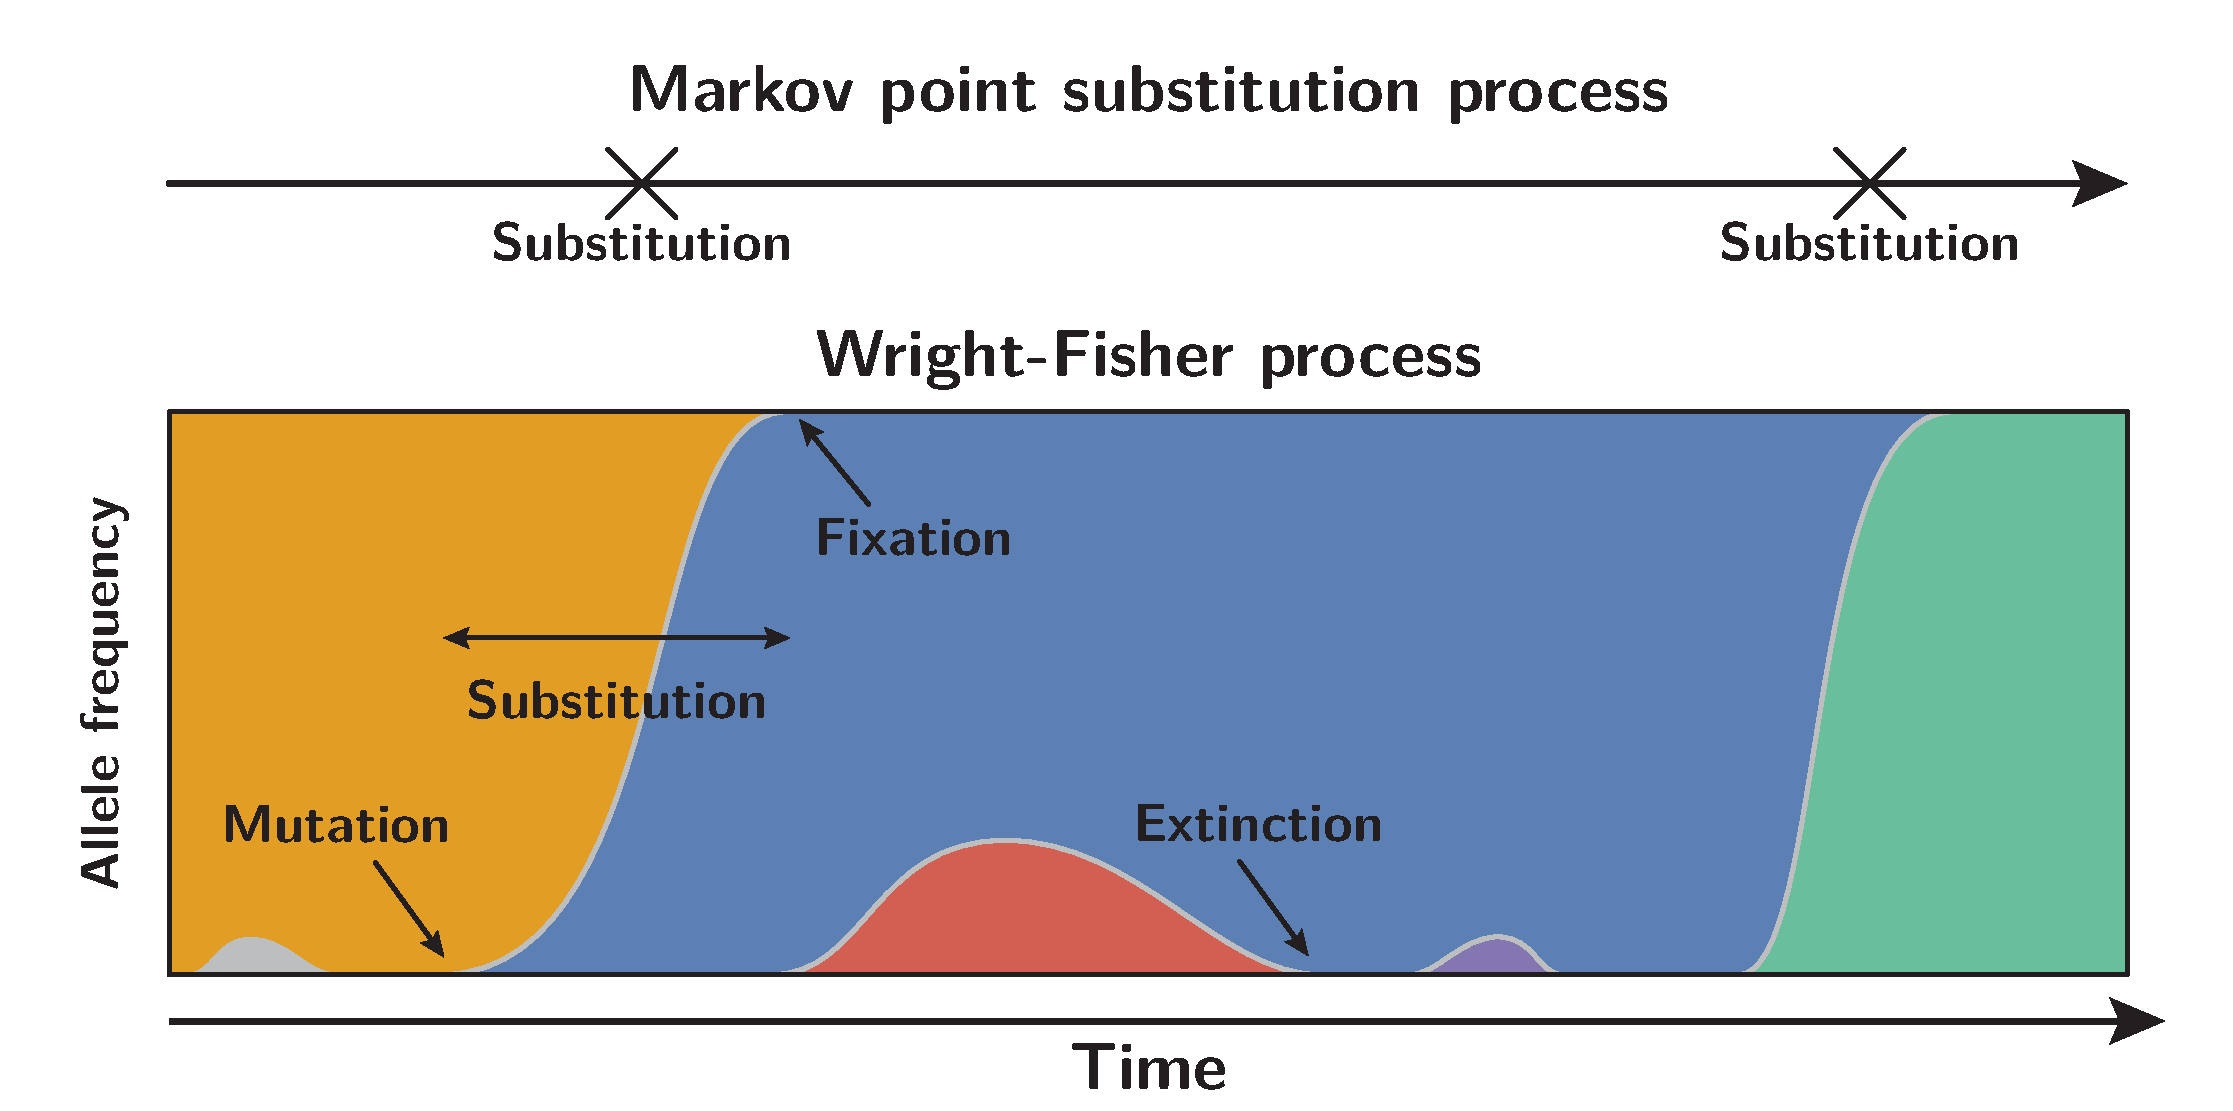
\includegraphics[width=0.6\textwidth]{figures/point-process.pdf}
	\caption[Mutation-selection point substitutions]{Mutation-selection point substitutions models. The trajectory of alleles inside a population is collapsed into a single point \gls{substitution} process. This approximation is valid under low mutation rate such that a mutation originate uniquely whenever the gene is monomorphic (with a single allele).}
\end{figure}

\subsection{Substitution rate}
At each generation, the expectation for the number of possible mutants is $2\Ne u$, and each of these mutant have a probability $P_{\mathrm{fix}}$ to result in a \gls{substitution}.
Altogether, the rate of \gls{substitution} from \gls{allele} $A$ to $B$, denoted $Q_{A \to B}$, is equal to the rate of mutation ($\mu_{A \to B}$) multiplied by the probability of fixation of the mutation $P_{\mathrm{fix}}(s_{A \to B}, \Ne)$ and scaled by the number of possible mutants at each generation ($2\Ne$):
\begin{align}
Q_{A \to B} & = 2 \Ne \mu_{A \to B}  P_{\mathrm{fix}}(s_{A \to B}, \Ne) \\
\end{align}
It is important to note that the \gls{substitution} rate and mutation rate are in the same unit, such that this equation is valid whether the rate is measured in unit of time or generation.
As a convention, mutation rate measured in unit of generation is denoted $u$, and denoted $\mu$ when measured in unit of time. As a consequence, $\submatrix$ is measured in unit of time in our equation.

In the case of \gls{neutral} mutations, the probability of fixation is independent of the original and target sequence, and equal $1/2 \Ne$. Finally $Q_{A \to B}$ simplifies to: 
\begin{align}
Q_{A \to B} & = 2 \Ne \mu_{A \to B}  P_{\mathrm{fix}}(0, \Ne) \\
Q_{A \to B} & = 2 \Ne \mu_{A \to B} \dfrac{1}{2\Ne} \\
Q_{A \to B} & =  \mu_{A \to B}
\end{align}
In the case of selected mutations, the probability of fixation depends on the difference of log-fitness ($f_i$ and $f_j$) between the two alleles:
\begin{align}
Q_{A \to B} & = 2 \Ne \mu_{A \to B} P_{\mathrm{fix}}(s_{A \to B}, \Ne) \\
			& = 2 \Ne \mu_{A \to B}  \dfrac{2(f_{B} - f_{A})}{1 - \e^{4\Ne(f_{A} - f_{B})} } \\
			& = \mu_{A \to B} \dfrac{F_{B} - F_{A}}{1 - \e^{F_{A} - F_{B}} }\text{, where } F = 4\Ne f
\end{align}

It is important to note that if the difference of log-fitness tends to $0$, the \gls{substitution} rate equal the mutation rate:
\begin{align}
\lim_{|F_{B} - F_{A}| \to 0} Q_{A \to B} & = \mu_{A \to B}   \dfrac{F_{B} - F_{A}}{{1 - (1 + {F_{A} - F_{B}}) }} \nonumber \\
& =  \mu_{A \to B} 
\end{align}

Taken together, the \gls{substitution} rate which generates the \gls{substitution} history and ultimately the inter-specific diversity is parameterized solely by mutation, selection and drift.
Consequently, from a particular history of substitutions, one can theoretically estimate the parameter of selection, mutation and drift.

\subsection{Steady state at equilibrium}

A realization of the \gls{mc} for a long period of time results in given proportion of the time for which the \gls{mc} is in a specific states, where this proportion depends of the states fitnesses, the mutationnal process and $\Ne$.
Due to the ergodicity of the stochastic process, averaging over time is equivalent to determining the statistical equilibrium, given we can derive the probabilities of transitions between states of the \gls{mc}.
The mutation-selection \gls{substitution} process described by a \gls{mc} thus define a stationary distribution, and is time-reversible. 
More preciselyr, the probability $\pi_{A}$ to find the population in state $i$ is proportional to a function (also called a Boltzmann factor) that depends only on the fitness of sequence $i$, the population size, and details of the mutation process \citep{Sella2005,Mustonen2005}:
\begin{align}
\pi_{A} & = \dfrac{\sigma_{A}\e^{F_{A}}}{\sum_{B}\sigma_{B} \e^{F_{B}}},\\
\pi_{A} & = \sigma_{A}\e^{F_{A}} \mathcal{Z}^{-1}.
\end{align}
Where $\sigma_{A}$ is the stationary distribution of the mutational process alone which is also reversible and satisfy the detail balance:
\begin{align}
\sigma_{A} \mu_{A \to B} & = \sigma_{B} \mu_{B \to A}
\end{align}
At equilibrium, the evolutionary system reaches thus a Boltzmann-like distribution with $\Ne^{-1}$ playing the role of evolutionary temperature, and the log-fitness $f$ the role of energy\footnote{At high mutation rates, the quasi-species theory provides another analogy with statistical mechanics, in which the mutation rate plays the role of temperature.}.

One can verify that Markov process of substitutions is reversible and the detailed balanced is satisfied:
\begin{align}
\pi_{A} Q_{A \to B} & = \sigma_{A} \e^{F_{A}} \mathcal{Z}^{-1}  \mu_{A \to B} \dfrac{F_{B} - F_{A}}{1 - \e^{F_{A} - F_{B}} } \\
					& = \sigma_{A} \mu_{A \to B} \mathcal{Z}^{-1} \dfrac{F_{B} - F_{A}}{\e^{-F_{A}} - \e^{ - F_{B}} }\\
					& = \sigma_{B} \mu_{B \to A} \mathcal{Z}^{-1} \e^{F_{B}} \dfrac{F_{B} - F_{A}}{\e^{F_{B}-F_{A}} - 1 }\\
					& = \sigma_{B} \e^{F_{B}} \mathcal{Z}^{-1}  \mu_{B \to A} \dfrac{F_{A} - F_{B}}{ 1 - \e^{F_{B}-F_{A}}}\\
					& = \pi_{B}  Q_{B \to A}\\
\end{align}


\subsection{Relative \gls{substitution} rate} 

Probabilities of the stationary distribution allows to calculate all observable quantities of interest, such as mean fitness and mean \gls{substitution} rate, using standard probability theory.
One quantity of interest is the \gls{substitution} rate of selected mutations relative to that of \gls{neutral} mutations, called $\omega$.
From its definition, $\omega=1$ for genes or sites under \gls{neutral} evolution.
Most importantly, departure from $1$ would be interpreted as a signature of selection on sequences. 
First, $\omega>1$ is interpreted as a signal of adaptive recurrent evolution, where selection coefficient are on average positive.
On the other hand, $\omega<1$ is a signal of underlying purifying selection, such that the sequence is constrained and mutations proposed are on average a negatively selected.
Together, in the case of a mutation-selection point \gls{substitution} process, $\omega$ is defined as:
\begin{equation}
\omega = \dfrac{ \sum_{A} \pi_{A} \sum_{B} Q_{A \to B}}{\sum_{A} \pi_{A}  \sum_{B} \mu_{A \to B}},
\end{equation}
It worth noting that under the assumption of a static fitness landscape, a mutation-selection point \gls{substitution} process will result in $\omega \leq 1$. 

\begin{table}[H]
	\begin{center}
		\begin{tabular}{|l|c|c|c|}
			\hline
			Parameter & Symbol & Range \\
			\hline
			Scaled fitness & $F=4 \Ne f$ & finite, positive or negative \\
			Mutation rate per time & $\mu$ & $[10^{-11}, 10^{-8}]$ per site per year \\
			Substitution rate per time & $Q$ & $[10^{-11}, 10^{-8}]$ per site per year \\
			Equilibrium frequency & $\Pi$ & $[0, 1]$ \\
			Equilibrium frequency under mutation & $\sigma$ & $[0, 1]$ \\
			Relative \gls{substitution} rate & $\omega$ & $[0, 1]$ for purifying selection\\
			\hline
		\end{tabular}
	\end{center}
	\caption[Parameter of mutation-selection processes]{Parameter of mutation-selection processes}\label{table:params-mutsel}
\end{table}

\section{Mutation-selection analogy}

This section develops reflections on apparent similarities and analogies between the mutation-selection process and other processes present in a variety of scientific fields outside of evolutionary biology, displaying the same underlying mechanism and emerging properties, though with different name and aspiration.
This effort is made in the aim of giving another view of the mutation-selection process, such as to better appreciate and conceptualize its assumptions, its limits, and the respective role of the different components. 
Such attempts requires to boil down the mutation-selection mechanism into its core components, while at the same time rephrasing the description using lexicography outside of population-genetic such as to open new perceiving angles.

At the bottom, mutation is a process creating diversity, changing and moving the current viable state to a novel and unknown position, fundamentally allowing exploration of the state space.
On the other hand, selection is the criteria on which a new state is deemed a disrupting innovation or a nonviable alteration, and allow to determine which changes to exploit and which to filter out and discard based on its fitness.
Fundamentally, reducing the diversity created by the mutation process is the very essence of selection.
Finally, drift arbitrate between the creation and reduction of the two processes, it dictates how much exploration of novelty is permitted, and conversely how much exploitation of only the fittest states is granted.

I argue that this creation and reduction process is found at the core of several research disciplines, while the link between them is scarcely made \citep{Baeck1994, Eiben1998}. 

\subsection{Metropolis-Hasting sampling}
Obtaining a sequence of random samples from a probability distribution can be difficult, especially when the number of dimensions is high.
However, the Metropolis-Hasting procedure based on a Monte Carlo \gls{mc} can sample from any probability distribution, provided that we know how to compute the probability density, or even less restrictively any function proportional to the density \citep{Hastings1970}.
This stochastic procedure which is based on three steps bears many similarities with the mutation-selection process:
\begin{itemize}
	\item Generate a stochastic candidate from the current state, analogous to the mutation.
	\item Calculate the acceptance ratio as the ratio of the two densities, analogous to the selection coefficient of the mutated state.
	\item Stochastic acceptance or rejection based on the acceptance ratio, a process analogous to drift. 
\end{itemize}
Inherently, Metropolis-Hasting procedure is based on creating and subsequently reducing diversity, which allows to obtain a random sequence of samples from any distribution with a straightforward recipe, and is a critical tools in statistic and statistical physics.

\subsection{The exploration-exploitation dilemma}
Many mathematical, engineering and day-life problems are not about sampling a state space, but rather finding the optimal and best state given a criteria or a function to maximize.
Naturally, we would prefer deterministic (strictly reproducible) rather than stochastic optimizing strategies to search for an optimal state.
Unfortunately, whenever the state space is too large, often due to the curse of dimensionality, a greedy or heuristic search of an optimal state can performs atrociously \citep{Bellman1966}.
In high dimensional space, stochastic optimization tools have been deemed very valuable, such as stochastic gradient decent or so called evolutionary algorithm \citep{Russell2010,Vikhar2017}.
Inherently, they are based on two processes, one is stochastically creating diversity and exploring the state space, while the other is filtering the explored states and thus reducing the diversity.

In the constrained case of a finite number of time or attempts to find the best outcome overall, the problem is best described by the multi-armed bandit problem. The name comes from imagining a gambler at a row of slot machines (sometimes known as one-armed bandits), where each slot machine provides a random reward from a probability distribution specific to that machine. The player has to decide which machines to play, how many times to play each machine and in which order to play them, and whether to continue with the current machine or try a different machine, such as to maximize the sum of rewards earned through a sequence of trials.
The gambler faces a dilemma at each trial, either reducing his regret by exploiting the best arm, or gaining information through exploration of other arms.
The best strategy to solved this dilemma can be mathematically derived in numerous cases, and encompass a mixing strategies with a defined ratio of exploration and exploitation \citep{Auer2002,Kocsis2006,Furnkranz2006}.
This problem is far from be only theoretical, and has be used to explain a multitude of phenomena, such as the movement of animals in novel landscapes, the most efficient resource allocation for a start-up company, the effects of age on knowledge acquisition in humans, and in search of the most efficient treatment in clinical trials (hence the name a clinical arm) \citep{Berger-Tal2014, March}. 
An other application of the exploration-exploitation dilemma is AlphaGo, the first computational program mastering the board game go at the professional 9-dan level in 2017, and out-compete Ke Jie, the world n°1 ranked player at the time \citep{Silver2017, Silver2018}.
AlphaGo has often been publicized and hyped in various media outlets that this feat was possible due to machine learning, more specifically due to convolutionnal neural networks.
However, it is more scarcely mentioned that AlphaGo neural network is combined with an exploration-exploitation algorithm, or more specifically Monte Carlo tree search. 
In practice, the convolutionnal neural network is used as a criteria to measure the advantage of a board configuration\footnote{Convolutionnal neural networks also use a stochastic gradient descend to reach convergence, inherently leveraging stochastic exploration and exploitation procedure to optimize the parameters of the neural network.}, but the different moves and path probed and trimmed is done via an exploration-exploitation procedure. 


Altogether, exploration and exploitation, creation and reduction, mutation and selection, are different names that encompass the inherently same process efficiently sampling and optimizing whenever the state is too large to be traversed.
I argue that scientific research endeavor is also a exploration-exploitation dilemma, which is arguably externally pressured to pursue exploitation, through funding of impactful research and a \textit{publish-or-perish} systemic culture in early career stage.

% As a side note, it appears that drift and selection are actually confounded, they are both on the side of exploitation, not on exploration.
As a side note, mutation is a necessary process of evolution, while sexe is not mandatory but increase the diversity of genomes between generations.
Arguably, studying evolution while disregarding mutation is a sufficient approximation whenever mutation rate and number of generations is low, which is developed thoroughly through the whole field of quantitative genetics.
Sex and mutation are both generating new states and are part of the more general exploration facet.
This explains why sex is favored in fluctuating environments.

I argue that evolutionary biologists, studying and leveraging the pervasive process of mutation and selection, can gain knowledge by recruiting insight and developments from other fields, much like there as been many crossover between economics and evolution in the context of game theory.\footnote{Game theory had originally been developed to model economic actors behavior and strategies \citep{VonNeumann1947}, while latter being emerging as the framework of evolutionary dynamics, which explains the emergence of altruistic behaviours in Darwinian evolution \citep{Smith1973, Smith1982, Nowak2006}.}.

%As an example of such insight from exploration-exploitation dilemma is on the understanding of relationship between mutation rate and chromosome size.
%It has been observed that organism with a low mutation rate (per site per generation) tend also to have a long chromosome size, such that the product of genome size and mutation rate is constant (Drake's rule).
%A resolution of this conundrum is that between generation, the genetical diversity of offsprings must balance the trade-off between being the same of their parents, or innovative.
%This trade off between exploration and exploitation seems to be shared by many organisms.



\chapter{Selection in protein coding {DNA} sequences}
{
	\hypersetup{linkcolor=GREYDARK}
	\minitoc
}
\label{sec:selection}
Evolutionary trajectory of sequences depends on the forces of mutation, selection and drift, which acts conjointly such that each one of them must be well studied and understood.
However, the previous chapter remained so far elusive on selection, and did not yet question what determines the strength of selection.
More precisely, molecular evolution requires either a given selection coefficient associated to mutation, or that the fitness of each particular sequence to be defined.
In other word, the relationship between sequence and fitness must be elucidated, which is the focus of the present chapter in the special case of protein coding \acrshort{DNA} sequence.
It will seek to clarify the relationship between protein sequence, protein thermodynamic, protein function, and organismal fitness, such as to derive the selective pressures shaping proteins coding \acrshort{DNA} sequences.
It is also important to emphasize whether they are general principles, or do this relationship between sequence and fitness depends on the specific protein, organism, and environment.
To this aims, this chapter will first present the genetic code and classical phylogenetic \glspl{codon} models, which can quantify the strength of selection acting on proteins trough an aggregate parameter (called $\omega$ or $\dnds$).
Application of these phylogenetic models to empirical \acrshort{DNA} alignment provides insight on the variation of selective strength between different orthologous genes, between sites of the same protein, or between branches of the phylogenetic tree.
Subsequently, physico-chemical constrains of proteins and thermodynamics models of protein selection are related to these empirical results.
Finally, given the results on empirical data, generalization of \gls{codon} models into the context of fitness landscapes are presented.

\section{Protein coding \acrshort{DNA} sequences}

Proteins have a variety of molecular and cellular roles, they are the enzymes that catalyses chemical bonds, they regulate cell processes and control their rates, they carry signals within the cell and across membranes, they bind and transport small molecules, they form cellular structures, and so on.
This variety of roles is accomplished by a variety of three-dimensional shapes.
A protein's three-dimensional shape is in turn determined by the linear one-dimensional sequence of amino-acids, with their size ranging from fewer than $20$ to more than $5000$ amino acids, with an average of about 350 amino-acids.
Just as \acrshort{DNA} is oriented because of the asymetry of nucleotides, proteins are oriented due to asymetry of amino-acids, one end is called \gls{N-ter} and the other end C-terminus, and each amino-acid will interact with the other amino-acids in its spatial vicinity. 

Although each of the 20 different amino acids has unique biochemical properties, they can be classified broadly into four categories determining their solubility and acidity (classification is given in table \ref{table:genetic_code}).
Charged amino-acids can be either basic (positively charged) or acidic (negatively charged).
On the other hand, non charged amino-acids can however be polar due to an uneven charge distribution, such that they can form hydrogen bonds with water.
Consequently, polar amino acids are called hydrophilic, and are often found on the outer surface of folded proteins.
Also, non charged amino-acids can have a uniform charge distribution, and do not form hydrogen bonds with water.
Reciprocally, these non polar amino-acids are called hydrophobic and tend to be found in the core of folded proteins.

\subsection{Genetic code}

Because the $20$ letter alphabet of proteins is different to the $4$ letter alphabet of nucleic acid (DNA and RNA), there is not a one-to-one correspondence between the two alphabets.
Instead, amino acids are encoded by \glspl{codon}, a consecutive sequences of 3 nucleotides, yielding $4^3=64$ possible permutations, more than sufficient to encode the 20 different amino acids.
Moreover, three stop \glspl{codon} signals termination of the protein, such that 61 of the 64 \glspl{codon} are used to encode amino acids.
Since there are 61 coding \glspl{codon} and only 20 amino acids, there is a necessary redundancy in the code.
Thus, amino-acids are encoded by synonymous \glspl{codon}, which are interchangeable in the sense of producing the same amino acid, with the notable exception of methionine and tryptophan.
Altogether, the \acrshort{DNA} genetic code translating \gls{codon} to amino-acids, which is used almost universally by all organisms is given in table \ref{table:genetic_code}.

\begin{table}[H]
	\centering
	\noindent\adjustbox{max width=\textwidth}{%
		\begin{tabular}{|c||l|c|l|c|l|c|l|c||c|}
			\hhline{|-||-|-|-|-|-|-|-|-||-|}
			& \multicolumn{2}{c|}{\textbf{T}} & \multicolumn{2}{c|}{\textbf{C}} & \multicolumn{2}{c|}{\textbf{A}} & \multicolumn{2}{c||}{\textbf{G}} & \\
			\hhline{=#========#=}
			\multirow{4}{*}{\textbf{T}} & TTT & \cellcolor{Nonpolar} & TCT & \cellcolor{Polar} & TAT & \cellcolor{Polar} & TGT & \cellcolor{Polar} & \textbf{T} \\
			\cline{2-2} \cline{4-4} \cline{6-6} \cline{8-8} \cline{10-10}
			& TTC & \cellcolor{Nonpolar} \multirow{-2}{*}{Phenylalanine (Phe/P)} & TCC & \cellcolor{Polar} & TAC & \cellcolor{Polar} \multirow{-2}{*}{Tyrosine (Tyr/Y)} & TGC & \cellcolor{Polar} \multirow{-2}{*}{Cysteine (Cys/C)} & \textbf{C} \\
			\hhline{|~||-|-|-|>{\arrayrulecolor{Polar}}->{\arrayrulecolor{black}}|-|-|-|-||-|}
			& TTA & \cellcolor{Nonpolar} & TCA & \cellcolor{Polar} & TAA & \cellcolor{Stop} Stop (Ochre) & TGA & \cellcolor{Stop} Stop (Opal) & \textbf{A} \\
			\hhline{|~||-|>{\arrayrulecolor{Nonpolar}}->{\arrayrulecolor{black}}|-|>{\arrayrulecolor{Polar}}->{\arrayrulecolor{black}}|-|-|-|-||-|}
			& TTG & \cellcolor{Nonpolar} & TCG & \cellcolor{Polar} \multirow{-4}{*}{Serine (Ser/S)} & TAG & \cellcolor{Stop} Stop (Amber) & TGG & \cellcolor{Nonpolar} Tryptophan (Trp/W) & \textbf{G} \\
			\hhline{|-||-|>{\arrayrulecolor{Nonpolar}}->{\arrayrulecolor{black}}|-|-|-|-|-|-||-|}
			\multirow{4}{*}{\textbf{C}} & CTT & \cellcolor{Nonpolar} & CCT & \cellcolor{Nonpolar} & CAT & \cellcolor{Basic} & CGT & \cellcolor{Basic} & \textbf{T} \\
			\cline{2-2} \cline{4-4} \cline{6-6} \cline{8-8} \cline{10-10}
			& CTC & \cellcolor{Nonpolar} & CCC & \cellcolor{Nonpolar} & CAC & \cellcolor{Basic} \multirow{-2}{*}{Histidine (His/H)} & CGC & \cellcolor{Basic} & \textbf{C} \\
			\hhline{|~||-|>{\arrayrulecolor{Nonpolar}}->{\arrayrulecolor{black}}|-|>{\arrayrulecolor{Nonpolar}}->{\arrayrulecolor{black}}|-|-|-|>{\arrayrulecolor{Basic}}->{\arrayrulecolor{black}}||-|}
			& CTA & \cellcolor{Nonpolar} & CCA & \cellcolor{Nonpolar} & CAA & \cellcolor{Polar} & CGA & \cellcolor{Basic} & \textbf{A} \\
			\cline{2-2} \cline{4-4} \cline{6-6} \cline{8-8} \cline{10-10}
			& CTG & \cellcolor{Nonpolar} \multirow{-6}{*}{Leucine (Leu/L)} & CCG & \cellcolor{Nonpolar} \multirow{-4}{*}{Proline (Pro/P)} & CAG & \cellcolor{Polar} \multirow{-2}{*}{Glutamine (Gln/Q)} & CGG & \cellcolor{Basic} \multirow{-4}{*}{Arginine (Arg/R)} & \textbf{G} \\
			\hhline{|-||-|-|-|-|-|-|-|-||-|}
			\multirow{4}{*}{\textbf{A}} & ATT & \cellcolor{Nonpolar} & ACT & \cellcolor{Polar} & AAT & \cellcolor{Polar} & AGT & \cellcolor{Polar} & \textbf{T} \\
			\cline{2-2} \cline{4-4}\cline{6-6} \cline{8-8} \cline{10-10}
			& ATC & \cellcolor{Nonpolar} & ACC & \cellcolor{Polar} & AAC & \cellcolor{Polar} \multirow{-2}{*}{Asparagine (Asn/N)} & AGC & \cellcolor{Polar} \multirow{-2}{*}{Serine (Ser/S)} & \textbf{C} \\
			\hhline{|~||-|>{\arrayrulecolor{Nonpolar}}->{\arrayrulecolor{black}}|-|>{\arrayrulecolor{Polar}}->{\arrayrulecolor{black}}|-|-|-|-||-|}
			& ATA & \cellcolor{Nonpolar} \multirow{-3}{*}{Isoleucine (Ile/I)} & ACA & \cellcolor{Polar} & AAA & \cellcolor{Basic} & AGA & \cellcolor{Basic} & \textbf{A} \\
			\hhline{|~||-|-|-|>{\arrayrulecolor{Polar}}->{\arrayrulecolor{black}}|-|>{\arrayrulecolor{Basic}}->{\arrayrulecolor{black}}|-|>{\arrayrulecolor{Basic}}->{\arrayrulecolor{black}}||-|}
			& ATG & \cellcolor{Nonpolar} Methionine (Met/M) & ACG & \cellcolor{Polar} \multirow{-4}{*}{Threonine (Thr/T)} & AAG & \cellcolor{Basic} \multirow{-2}{*}{Lysine (Lys/K)} & AGG & \cellcolor{Basic} \multirow{-2}{*}{Arginine (Arg/R)} & \textbf{G} \\
			\hhline{|-||-|-|-|-|-|-|-|-||-|}
			\multirow{4}{*}{\textbf{G}} & GTT & \cellcolor{Nonpolar} & GCT & \cellcolor{Nonpolar} & GAT & \cellcolor{Acidic} & GGT & \cellcolor{Nonpolar} & \textbf{T} \\
			\cline{2-2} \cline{4-4} \cline{6-6} \cline{8-8} \cline{10-10}
			& GTC & \cellcolor{Nonpolar} & GCC & \cellcolor{Nonpolar} & GAC & \cellcolor{Acidic} \multirow{-2}{*}{Aspartic acid (Asp/D)} & GGC & \cellcolor{Nonpolar} & \textbf{C} \\
			\hhline{|~||-|>{\arrayrulecolor{Nonpolar}}->{\arrayrulecolor{black}}|-|>{\arrayrulecolor{Nonpolar}}->{\arrayrulecolor{black}}|-|-|-|>{\arrayrulecolor{Nonpolar}}->{\arrayrulecolor{black}}||-|}
			& GTA & \cellcolor{Nonpolar} & GCA & \cellcolor{Nonpolar} & GAA & \cellcolor{Acidic} & GGA & \cellcolor{Nonpolar} & \textbf{A} \\
			\cline{2-2} \cline{4-4} \cline{6-6} \cline{8-8} \cline{10-10}
			& GTG & \cellcolor{Nonpolar} \multirow{-4}{*}{Valine (Val/V)} & GCG & \cellcolor{Nonpolar} \multirow{-4}{*}{Alanine (Ala/A)} & GAG & \cellcolor{Acidic} \multirow{-2}{*}{Glutamic acid (Glu/E)} & GGG & \cellcolor{Nonpolar} \multirow{-4}{*}{Glycine (Gly/G)} & \textbf{G} \\
			\hhline{|-||-|-|-|-|-|-|-|-||-|}
	\end{tabular}}
	\caption[The Genetic Code]{
		The genetic code \acrshort{DNA} table translating \glspl{codon} into amino-acids.
		Amino-acids are represent into $4$ categories based on the electrochemical properties.
		Non-polar in yellow (\textcolor{Nonpolar}{\ding{110}}), polar in green (\textcolor{Polar}{\ding{110}}), basic in blue (\textcolor{Basic}{\ding{110}}) and finally acidic in red (\textcolor{Acidic}{\ding{110}}).
		Stop \glspl{codon} are represented in black (\textcolor{Stop}{\ding{110}}).
		The synonymous \glspl{codon} encoding for the same amino-acid are usually different by their third \gls{codon} position, the wooble base.
	}
	\label{table:genetic_code}
\end{table}

Biochemical translation from \gls{codon} to amino-acid mechanistically emanates from transfer \acrshort{RNA} (\acrshort{tRNA}).
More precisely, \glspl{codon} binds to \acrshort{tRNA} via an anticodon, three consecutive bases that are complementary and antiparallel to the associated \gls{codon}.
On the other end, \acrshort{tRNA} structure complexes uniquely with one the $20$ amino acid, where the catalytic reaction is performed by aminoacyl-tRNA synthetase \citep{Rich1976}.
As a result, \acrshort{tRNA} genes along with aminoacyl-tRNA synthetase genes constitute the machinery necessary for translating \glspl{codon} into amino-acids .
However, there is not a one-to-one correspondence between the $61$ \glspl{codon} and \acrshort{tRNA} genes.
First, the set of unique sequence of anticodon found in tRNAs genes is actually lower than $61$, and depends on the species but varies from $41$ to $55$ \citep{Goodenbour2006}.
This subset of anticodon sequences necessary to binds all $61$ \glspl{codon} is due to non canonical base pairing\footnote{Canonical base pairing are A-U and G-C, where thymin (T) is replaced by uracil (U) in RNA}.
More precisely, the first two positions in the \gls{codon} bond strongly to the anticodon of the \acrshort{tRNA} (second and third positions), while the third base of the \gls{codon} can be subject to non standard pairing with the first base of the anticodon.
If the anticodon contains a guanine at first position, \glspl{codon} with either U or C at the third position can bounds to this anticodon, and this phenomenon explains why there is not any non-synonymous {transition} from only U to C at third position, and why synonymous \glspl{codon} usually end with T or C.
Also, if the anticodon contains an Inosine at first position, \glspl{codon} with either C, U or A at the third position can bounds to this anticodon, such that for example Leucine encoded by three \gls{codon} (AUU, AUC, AUA) can be bounded by the unique anticodon IAU.
Altogether, non-standard pairing explains why the number of unique anticodons is lower than the number of possible \glspl{codon}, and also explains some part of the structure of the genetic code.

Secondly, \acrshort{tRNA} genes with the same amino-acid binding site and anticodon, which are called isoacceptor \acrshort{tRNA}, may vary in other parts of the \acrshort{tRNA} sequence.
Effectively, many genes can codes for the same isoacceptor \acrshort{tRNA}, where each gene can display varying efficiency and errors in translation, adding a layer of regulation to the process of protein synthesis \citep{Lowe1997,Chan2008,Juhling2008,Lin2019}.
As a result, in some genes some \glspl{codon} are more frequently represented than other possible synonymous \glspl{codon}, an effect named \gls{codon} usage bias.
For genes that are expressed at high levels, the \gls{codon} use is biased in favor of the \glspl{codon} that have an high \acrshort{tRNA} concentration in the cell, ultimately increasing the expression rate and decreasing the rate of mistranslation by reducing the time of occupancy of an open site.
Thus, at a fine-grained molecular scope, a synonymous change can influence mRNA stability, splicing process and protein-folding during translation \citep{Plotkin2011, Rak2018}.
However in the scope of this manuscript, such selection between synonymous \glspl{codon} will not be considered, and selection for proteins will be framed at the amino-acid level in first approximation, and mutation at the nucleotide level.
\begin{table}[H]
	\centering
	\noindent\adjustbox{max width=\textwidth}{%
	\begin{tabu}{|c||c|c|c|c|c|c|c|c|c|c|c|c|c|c|c|c|c|c|c|c|}
		\hline & \textbf{K} & \textbf{N} & \textbf{T} & \textbf{R} & \textbf{S} & \textbf{I} & \textbf{M} & \textbf{Q} & \textbf{H} & \textbf{P} & \textbf{L} & \textbf{E} & \textbf{D} & \textbf{A} & \textbf{G} & \textbf{V} & \textbf{Y} & \textbf{C} & \textbf{W} & \textbf{F}\\
		\hline
		\hline \textbf{K} & - & 4 & 2 & 2 & 0 & 1 & 1 & 2 & 0 & 0 & 0 & 2 & 0 & 0 & 0 & 0 & 0 & 0 & 0 & 0\\
		\hline \textbf{N} & - & - & 2 & 0 & 2 & 2 & 0 & 0 & 2 & 0 & 0 & 0 & 2 & 0 & 0 & 0 & 2 & 0 & 0 & 0\\
		\hline \textbf{T} & - & - & - & 2 & 6 & 3 & 1 & 0 & 0 & 4 & 0 & 0 & 0 & 4 & 0 & 0 & 0 & 0 & 0 & 0\\
		\hline \textbf{R} & - & - & - & - & 6 & 1 & 1 & 2 & 2 & 4 & 4 & 0 & 0 & 0 & 6 & 0 & 0 & 2 & 2 & 0\\
		\hline \textbf{S} & - & - & - & - & - & 2 & 0 & 0 & 0 & 4 & 2 & 0 & 0 & 4 & 2 & 0 & 2 & 4 & 1 & 2\\
		\hline \textbf{I} & - & - & - & - & - & - & 3 & 0 & 0 & 0 & 4 & 0 & 0 & 0 & 0 & 3 & 0 & 0 & 0 & 2\\
		\hline \textbf{M} & - & - & - & - & - & - & - & 0 & 0 & 0 & 2 & 0 & 0 & 0 & 0 & 1 & 0 & 0 & 0 & 0\\
		\hline \textbf{Q} & - & - & - & - & - & - & - & - & 4 & 2 & 2 & 2 & 0 & 0 & 0 & 0 & 0 & 0 & 0 & 0\\
		\hline \textbf{H} & - & - & - & - & - & - & - & - & - & 2 & 2 & 0 & 2 & 0 & 0 & 0 & 2 & 0 & 0 & 0\\
		\hline \textbf{P} & - & - & - & - & - & - & - & - & - & - & 4 & 0 & 0 & 4 & 0 & 0 & 0 & 0 & 0 & 0\\
		\hline \textbf{L} & - & - & - & - & - & - & - & - & - & - & - & 0 & 0 & 0 & 0 & 6 & 0 & 0 & 1 & 6\\
		\hline \textbf{E} & - & - & - & - & - & - & - & - & - & - & - & - & 4 & 2 & 2 & 2 & 0 & 0 & 0 & 0\\
		\hline \textbf{D} & - & - & - & - & - & - & - & - & - & - & - & - & - & 2 & 2 & 2 & 2 & 0 & 0 & 0\\
		\hline \textbf{A} & - & - & - & - & - & - & - & - & - & - & - & - & - & - & 4 & 4 & 0 & 0 & 0 & 0\\
		\hline \textbf{G} & - & - & - & - & - & - & - & - & - & - & - & - & - & - & - & 4 & 0 & 2 & 1 & 0\\
		\hline \textbf{V} & - & - & - & - & - & - & - & - & - & - & - & - & - & - & - & - & 0 & 0 & 0 & 2\\
		\hline \textbf{Y} & - & - & - & - & - & - & - & - & - & - & - & - & - & - & - & - & - & 2 & 0 & 2\\
		\hline \textbf{C} & - & - & - & - & - & - & - & - & - & - & - & - & - & - & - & - & - & - & 2 & 2\\
		\hline \textbf{W} & - & - & - & - & - & - & - & - & - & - & - & - & - & - & - & - & - & - & - & 0\\
		\hline \textbf{F} & - & - & - & - & - & - & - & - & - & - & - & - & - & - & - & - & - & - & - & -\\
		\hline
	\end{tabu}}
\caption[Amino-acids adjacency matrix]{
Number of possible one nucleotide non-synonymous {transitions} between amino-acids, integrating over the underlying \glspl{codon}.
For all the possible $190$ pairs of amino-acids, only $75$ pairs contains at least one non-synonymous {transition}.
}
\label{table:adjacency}
\end{table}
Because mutations are at the nucleotide level and affect only one base, any \gls{codon} can have at most $9$ possible {transitions} to another \glspl{codon} as illustrated in the left panel of figure \ref{fig:graph-codons-aa}.
Moreover, it is possible that some pairs of amino-acids are not accessible through a single non-synonymous {transition} between the underlying \glspl{codon} as illustrated in the right panel of figure \ref{fig:graph-codons-aa}.
In fact, most pairs of amino-acids requires at least two non-synonymous {transitions} ($114$ pairs), in comparison to pairs of amino-acids that are accesible trough a single non-synonymous {transition} ($75$ pairs).

\begin{figure}[htbp!]
	\centering
		\begin{minipage}{0.49\linewidth}
			\includegraphics[width=\linewidth, page=1]{figures/gt-codon-tab20b.pdf}
		\end{minipage}%
		\hfill
		\begin{minipage}{0.49\linewidth}
			\includegraphics[width=\linewidth, page=1]{figures/gt-aa-tab20b.pdf}
		\end{minipage}

	\caption[Graphs of \gls{codon} and amino-acid transitions]{
		\label{fig:graph-codons-aa}
		Graphs of possible one nucleotide {transition} between \gls{codon} (left panel) and between amino-acid (right panel).
		Nodes corresponds to \glspl{codon} (left panel) and amino-acid (right panel), where their color pictures the encoded amino-acid.
		Additionanly, for amino-acids the size of nodes represent the number of underlying \glspl{codon}.
		An edge between two \glspl{codon} depicts a one nucleotide {transition}, such that a \gls{codon} can have at most $9$ possible {transitions}.
		Similarly, an edge between two amino-acids correspond to a one nucleotide non-synonymous {transition} between the underlying \glspl{codon}, and the weight of the edges represent the number such possible {transitions}.
		Non-synonymous {transition} are represented in colored gradient, while synonymous {transitions} are depicted in black.
		The graph of the $61$ \glspl{codon} contains $263$ {transitions}, $67$ of them are syonymous while $196$ are non-synonymous.
		The radius of the graph is three, such that the most distant amino-acids are at most three {transition} away.
		Codons encoding for the same amino-acid are all fully connected by synonymous changes, expect for Serine where a {transition} for (TCT, TCG, TCC,	TCA) to (AGT, AGC) requires passing trought another amino-acid, hence a least two non-synonymous {transitions}.
		From the perspective of amino-acids, the graph of the $20$ amino-acids contains $75$ non-synonymous {transitions}.
		The graph is not fully connected and do not form a clique. Moreover, the graph radius equal to three because a {transition} from Methione to Tyrosine requires at least three non-synonymous {transitions}.
		Altogether, for all the possible $190$ pairs of amino-acids, $114$ pairs requires at least two non-synonymous {transitions}, and one pair (M-Y) requires at least three non-synonymous {transitions}.
	}
\end{figure}

\subsection{Codon \gls{substitution} models}
Under the approximation that selection occurs for protein, designing \gls{substitution} models at the amino-acid level has the major shortcoming of not taking into account that the underlying mutation process occurs at the nucleotide level.
Conversely, studying evolution of protein coding \acrshort{DNA} sequences only at the nucleotide level, while disregarding the genetic code neglects the consequences that nucleotide variation can have onto protein sequences.
These shortcomings are both addressed by \gls{codon} models, where the complexity of the genetic code is seen as an asset rather than an encumbrance.
Indeed the redundancy in the genetic code can be leveraged to disentangle mutation and selection in protein coding \acrshort{DNA} sequences, under the approximation that selection occurs at the protein level in first approximation, while the mutation process occurs at the \acrshort{DNA} level.
The genetic code allows to split mutations into synonymous and non-synonymous mutations, where synonymous mutations are deemed \gls{neutral}, and non-synonymous mutations are considered under selection \citep{Muse1994,Goldman1994}.

Following the formalism of \gls{codon} models pioneered by \citet{Muse1994}, the $4 \times 4$ mutation matrix $\Mutmatrix$ at the nucleotide level is defined as:
\begin{equation}
\label{eq:mutrates}
\Mutmatrix = \begin{pmatrix}
- & {\mutmatrix_{AC}} & 		{\mutmatrix_{AG}} & 		{\mutmatrix_{AT}} \\
{\mutmatrix_{AC}} & - & {\mutmatrix_{CG}} &		{\mutmatrix_{CT}} \\
{\mutmatrix_{AG}} & 		{\mutmatrix_{CG}} & - & {\mutmatrix_{GT}} \\
{\mutmatrix_{AT}} & 		{\mutmatrix_{CT}} & 		{\mutmatrix_{GT}} & -
\end{pmatrix},
\end{equation}
Grouping nucleotides into \glspl{codon}, mutation rate from \gls{codon} $\ci$ to $\cj$ thus depends on the underlying nucleotide change between the \gls{codon}, if $\ci$ to $\cj$ are only a mutation away, $\nucitoj$ denotes the nucleotide change between the \glspl{codon} and the mutation rate from \gls{codon} $\ci$ to $\cj$ is:
\begin{equation}
\mu_{\itoj} = 
\begin{dcases}
 \mutmatrix_{\nucitoj} \text{ if $\ci$ and $\cj$ are one mutation away,} \\
 0 \text{ else.}
\end{dcases}
\end{equation}

At the \gls{codon} level, synonymous mutations are deemed \gls{neutral} and the rate of \glspl{synonymous} ${\submatrix_{\itoj}}$ is equal to the mutation rate: 
\begin{align}
\submatrix_{\itoj} & = \mu_{\itoj} \\
				  & = \mutmatrix_{\nucitoj}
\end{align}

Conversely, non-synonymous mutations are considered under selection, where their probability of fixation is stretched by a factor $\omega$, and their \gls{substitution} rate is:
\begin{align}
\submatrix_{\itoj} & = \omega \mu_{\itoj} \\
					& = \omega \mutmatrix_{\nucitoj}.
\end{align}
All non-synonymous mutations are considered equivalent, and $\omega$ encompass the average strength of selection exercised on them.
Most importantly, $\omega>1$ is absorbing the signals of an excess in the rate of \glspl{non-synonymous}, indicating that the protein is under adaptive evolution.
Conversely, a default of \glspl{non-synonymous}, leading to $\omega<1$, means the protein is under purifying selection.


Because of this definition, $\omega$ identifies with the rate of \glspl{non-synonymous} over the rate of \glspl{synonymous}, termed $\dnds$.

Throughout this manuscript, the term $\dnds$ will be used to identify the estimation of $\omega$ from protein coding \acrshort{DNA} sequence alignment under the original model of \citet{Muse1994}.
To note, $\omega$ can also be parameterized as function of the average scaled selection coefficient:
\begin{align}
\omega & = \dfrac{S}{1 - \e^{-S}} \text{, where }\\
& \Rightarrow	\begin{dcases}
	S > 0 \iff \omega > 1 \\
	S = 0 \iff \omega = 1 \\
	S < 0 \iff \omega < 1
	\end{dcases}
\end{align}

Altogether, the $61$-by-$61$ \gls{codon} \gls{substitution} matrix of \citet{Muse1994} is defined entirely by the mutation matrix ($\Mutmatrix$), $\omega$ and the genetic code:
\begin{equation}
\begin{dcases}
\submatrix_{\itoj} & = 0 \text{ if $\ci$ and $\cj$ are not one mutation away} \\
\submatrix_{\itoj} & = \mutmatrix_{\nucitoj} \text{ if $\ci$ and $\cj$ are syonymous} \\
\submatrix_{\itoj} & = \omega \mutmatrix_{\nucitoj} \text{ if $\ci$ and $\cj$ are non-syonymous} \\
\submatrix_{\ci, \ci} & = - \sum_{\cj \neq \ci} \submatrix_{\itoj}
\end{dcases}
\label{eq:codon-models}
\end{equation}

It is important to note that under this model, the equilibrium frequencies of all \glspl{codon} are equal, and depends only on the equilibrium frequencies of nucleotides ($\sigma_{A}, \sigma_{C}, \sigma_{G}, \sigma_{T}$):
\begin{align}
\pi_{\ci} & = \dfrac{\sigma_{\ci[1]}\sigma_{\ci[2]}\sigma_{\ci[3]}}{\sum_{\cj}\sigma_{\cj[1]}\sigma_{\cj[2]}\sigma_{\cj[3]} } \\
 & = \dfrac{\sigma_{\ci[1]}\sigma_{\ci[2]}\sigma_{\ci[3]}}{(1 - \sigma_{T}\sigma_{A}\sigma_{A} - \sigma_{T}\sigma_{A}\sigma_{G} - \sigma_{T}\sigma_{G}\sigma_{A} )},
\end{align}
where $\ci[1]$ denotes the nucleotide at position $1$ of \gls{codon} $i$.

Moreover, the relative \gls{substitution} rate at equilibrium $\langle \nu \rangle$ defined by equation \ref{eq:relative-sub-rate}, if restricted to the subset of \glspl{non-synonymous}, identifies to $\omega$:
\begin{align}
\langle \nu \rangle & = \dfrac{ \sum_{\ci} \pi_{\ci} \sum_{\cj \in \NonSyn_{\ci}} Q_{\itoj}}{\sum_{\ci} \pi_{\ci} \sum_{\cj \in \NonSyn_{\ci}} \mu_{\itoj}} \\
					& = \dfrac{ \sum_{\ci} \pi_{\ci} \sum_{\cj \in \NonSyn_{\ci}} \omega \mu_{\itoj}}{\sum_{\ci} \pi_{\ci} \sum_{\cj \in \NonSyn_{\ci}} \mu_{\itoj}} \\
					& = \omega \dfrac{ \sum_{\ci} \pi_{\ci} \sum_{\cj \in \NonSyn_{\ci}} \mu_{\itoj}}{\sum_{\ci} \pi_{\ci} \sum_{\cj \in \NonSyn_{\ci}} \mu_{\itoj}} \\
					& = \omega, 
\end{align}
where $\NonSyn_{\ci}$ is the set of non-synonymous \glspl{codon} neighbors to \gls{codon} $\ci$.
This identity seems so far trivial and unnecessary, but will bear importance later when comparing this phenomenological model to mechanistic models of \gls{codon} \glspl{substitution}.


\section{Empirical relative rate of non-synonymous substitutions}
Models of \gls{codon} \glspl{substitution} can be to applied to protein coding \acrshort{DNA} sequences alignment to estimates the ratio of non-synonymous over \gls{synonymous} rates ($\dnds=\hat{\omega}$).
More precisely, these models can provides estimates of $\dnds$ for the whole gene, for a specific site or for a specific branch of the tree, and whether the sequence evolves under positive or negative selection.
However, in practice, protein are typically under a mix of adaptation and purifying selection, thus typically leading to an $\dnds<1$ even in the presence of positive selection.
Most importantly to the scope of this manuscript, they \gls{codon} models proved to be very valuable to quantify and asses the selective constrains imposed on protein coding sequences.

Importantly, different implementations of phylogenetic \gls{codon} models have been proposed, which parameterize the mutation matrix and the \gls{codon} frequencies in different way \citep{Muse1994, Goldman1994}, ultimately leading to variable fits of the data and different estimation of $\dnds$ on the same dataset. 
However, and fortunately, estimation of $\dnds$ has been proved to be largely insensitive to the underlying \gls{codon} models \citep{Spielman2018}, such that empirical estimation of $\dnds$ using different methods leads to comparable results.

\subsection{Variation across genes}

The increased availability of genomic data together with advancement of computing resources and algorithm prompted an extensive search for the major determining factor of a gene $\dnds$.
Surprisingly, the functional importance of a protein, widely thought to approximate the level of functional constraint, has only a minor role, whereas protein expression level (mRNA concentraion) is found to be a major determinant \citep{Zhang2015}.
Most importantly, this relationship is negative such that genes with high expression level are under stronger purifying selection, or lower $\dnds$ at the level of the gene \citep{Duret2000, Drummond2005a, Zhang2015}.
In unicellular organisms, the mRNA concentration of a gene varies across cell cycle stages and environments, but most studies used data collected from the mid-log phase of growth under rich media, which presumably reflect average concentrations across cell cycle stages.
In multicellular organisms, mRNA concentration data used are typically from the whole organism or are averaged from several examined tissues.
Because of the strong correlation between mRNA and protein concentrations, the negative correlation between protein concentration and evolutionary rate is also strong.

However, even for those proteins of comparable expression levels, their $\dnds$ still span several orders of magnitude \citep{Drummond2008}.
Abundance likewise cannot account for the quasi log-normal distribution of $\dnds$ among genes in a genome, a fact observed from bacteria, yeast, worm, fly, mouse, and humans.
These observations suggest that protein abundance, although a major determinant of $\dnds$, is not its only causal variable.

\subsection{Variation across sites}

Appart from variation across genes, the strength of selection is not typically homogeneous along the protein sequence, and it has been rapidly recognized that the parameter $\dnds$ should not be estimated globally over the entire sequence.
In so-called site-specific phylogenetic \gls{codon} models, $\dnds$ is allowed to vary across sites, either via a finite mixture \citep{Yang2001}, an infinite mixture \citep{Huelsenbeck2006}, or as random effects from a parametric distribution \citep{Lartillot2013}.
Site-specific models had been developed to detect specific site of the sequence under positive recurrent selection \citep{kosiol_patterns_2008}, with a $\dnds>1$, but also proved to be very valuable models to correlate selective pressure and bio-chemical properties os specific sites.

Similarly to search for the determining factors of $\dnds$ at the gene level, extensive search had been conducted at the site level, within a protein.
The major determinant of site-specific $\dnds$ proved to be relative solvent accessibility, where site with higher solvent accessibility display a lower $\dnds$ \citep{Ramsey2011}.
It was later shown that the number of native inter-residue contacts formed by a protein site, which is negatively correlated with the solvent accessibility, is a stronger predictor of site-specific $\dnds$ \citep{Yeh2013}.
Altogether, $\dnds$ changes dramatically between exposed and buried sites in such a way that buried sites tend to evolve more slowly than exposed sites \citep{Echave2016}.
Moreover, this relationship obtained by means of phylogenetic \gls{codon} models can be matched with experiment correlating protein site properties with allelic diversity within population.
In this context, relative solvent accessibility was also found to be a major determinant of adaptive evolution, with most adaptive mutations occurring at the surface of proteins \citep{Moutinho2019}.

The observations that surface residues of globular proteins undergo \gls{substitution} more rapidly than those in the core is generally attributed to the fact that natural selection imposes stronger constraints on buried sites.
It is well known that amino acid residues located inside a protein structure (that is, core residues) have more central roles than surface residues in protein folding stability.

Finally, it is important to keep in mind that selection differs in a way that depends on the specific source and target amino-acid involved in the {transition}.
As a consequence, a single parameter of selection (here $\dnds$) can not disentangle the specific importance of amino-acid chemical properties (polarity, volume, charge, and so on) since all non-synonymous {transitions} are considered equivalent in classical phylogenetic \gls{codon} models \citep{Dutheil2008}.

\subsection{Variation across branches}

Beside variation across genes and site, the strength of selection is not typically homogeneous along the phylogenetic tree, and it has also been recognized that the parameter $\dnds$ should be varying along the tree \citep{Yang1998}.
The motivation was to allow for $\dnds$ to be estimated only on a subset of the phylogeny, based on biological assumption.
For example, such models can detect an adaptive process ongoing during the divergence of one lineage, which can allow for the detection of the proteins responsible for speciation \citep{Yang2001, Zhang2004}.
Moreover, without \gls{prior} knowledge on biological divergence, branches can get clustered together based on their \gls{substitution} rates \citep{Dutheil2012a}.
However, \gls{substitution} rate is a continuous traits, and should evolve smoothly along the phylogeny, such that abrupt shifts are penalized \citep{Huelsenbeck2003,Seo2004}.
I this modeling approach, \gls{substitution} rate of given branch is log-normally distributed around the value of its parent branch, where the standard deviation is proportional to the branch size (in unit of time) \citep{Lartillot2011, Brevet2019}.
In other words, \gls{substitution} rate is seen as a log-Brownian motion along the phylogeny, where the process splits at every node of the tree. 

Similarly to search for the determining factors of $\dnds$ at the gene and site level, environmental variables or life-history traits that can vary between species have been investigated as factor determining $\dnds$ along the phylogeny \citep{Felsenstein1985,Romiguier2014}.
Integrative inference methods combining molecular sequences and lineage specific quantitative traits have also found that $\dnds$ correlates positively with traits such as longevity and body mass \citep{Lartillot2011, Figuet2017}.
Since lineage with a large body size and extended longevity typically correspond to low $\Ne$ \citep{Romiguier2014}, these empirical correlations suggest a negative correlation between $\dnds$ and $\Ne$, thus confirming the theoretical prediction of the \gls{nearly-neutral} theory of evolution.
However, the universality and robustness of the correlation between $\dnds$ and life-history traits is still debated \citep{Nabholz2013, Lanfear2014, Figuet2016}.

Naturally, both these space (site-specific) and time (branch-specific) refinements mentioned above where combined in so called branch-site models \citep{Yang2002, Zhang2004, Pond2011}.
The fine-grained tunning of site-branch models increased statistical power by seeking short and strong episodes of adaptive selection on a background of purifying selection.
However, in the case of Red-Queen processes ongoing on the protein, the episodes detected by branch-site models would merely be a small fraction of the underlying adaptation.
Indeed the overall tree is under adaptive process and one cannot contrast a branch to the rest of the tree.

%The selection coefficient are drawn from a distribution, known as distribution of fitness effects \citep{Welch2008}
%In Wilson, the fitness effect of a mutation is drawn from a fitness distribution that is solely function of $\Ne$, meaning ${P_{\mathrm{fix}}}$ is independent from the current sequence state.
%On the other hand, in the mutation-selection model proposed, the distribution of fitness effects is a function of the current state.
%
%Because its a distribution of fitness effects and not a fitness landscape, features of evolutionary trajectory such as transient positive selection is not represented.
%They are a generic representation of fitness, easily parameterized and inherently taking into account phenomenon such as epistasis.


\section{Protein biophysics}

The ability of a protein to performs its function depends on the stability of its 3-dimensional folding structure, but also on its ability to bind ligands and interact or no with other protein, both in terms of kinetic and stability.
Altogether, thermodynamics and kinetic of protein are expected to be related to its function, hence to selective constrains \citep{Bastolla2017}.
This section review the main relationship between protein biophysics and selection.
\textcolor{GREEN}{[I should be working on a better {transition} between classical \gls{codon} models and protein biophysics]}.
\subsection{Stability constrains}

First, a large body of evidence indicates that the stability of globular proteins is a target of natural selection \citep{Sikosek2014}.
The stability of a protein is determined by the Gibbs free energy of its folded states, in comparison to the free energy of the unfolded states.
Similarly to the mutation-selection Markov process defined in the previous chapter, it is possible to derive the equilibrium distribution of states, where fitness is analogous to the opposite of free energy (less energetic state are more stable) and population size to inverse temperature.
As a result, probabilities of observing a specific state, given by Boltzmann equation, is proportional to the exponential of free energy:
\begin{align}
p(G_F)\propto \e^{- G_F / T}.
\end{align}
In this context, mutations of the proteins stabilizes the protein only if the decrease the free energy of the folded states, more than they decrease the free energy of unfolded states.
For example, a {transition} to an amino-acid that decrease by the same amount the free energy of both folded and unfolded states will have no impact on the stability of the protein.
Theoretically, the stability of a protein can be computed with biophysical of protein, by modeling the atomic structure and the potential energy of contact between residues, computed using Schrodinger's equation and atomic orbitals \textcolor{GREEN}{[References needed]}.
On the other extreme, some models more crudely approximates the structure and dynamic of protein by 2-dimensional lattice models with regular pavement \textcolor{GREEN}{[References needed]}. 
In between these two extremes, many models can approximate with various degrees of liberties and parametrization the relationship from sequence to stability.
Broadly, {transition} from hydrophobic to hydrophilic amino-acids at the surface of protein results in increase stability, and conversely for the protein core.

If the relationship from protein sequence to protein stability is within reach and can be obtained with various degrees of approximations, relationship from stability to fitness is more elusive and difficult to apprehend.
First, it is known the protein stability relates to fitness, as demonstrated by a study of nearly 1000 mutations in beta-lactamase TEM-1 \citep{Jacquier2013}, or illustrated by the use of functional assays to identify stabilizing mutations \citep{Araya2012}.
However, it is not clear whether protein stability increases fitness by being more efficient, or whether it is the deleterious cytotoxic effect of unfolded proteins that result in purifying selection for destabilizing mutations.
Stability-constrained models that take into account negative design for destabilizing misfolded conformations.
At partial answer can be obtained by realizing that \citep{Berezovsky2007, Noivirt-Brik2009, Minning2013} predict that both the \gls{substitution} rate and the entropy are maximal not at exposed sites with few contacts, as observed, but at sites where the number of contacts is intermediate, which can accomodate both hydrophobic and polar amino acids and are predicted to be extremely tolerant to mutations \citep{Jimenez2018}.
On the other hand, when stability with respect to misfolding is not considered, stability-constrained models predict that the variability is maximal at exposed sites with few contacts \citep{Scherrer2012,Echave2015}, but these kinds of models overestimate both the tolerance to mutations and the average hydrophobicity at almost all positions \citep{Jimenez2018} and they score much worse than models that consider misfolding in \gls{likelihood} calculations \citep{Arenas2015a, Arenas2017}, so that models that consider misfolding have to be preferred.
These results support the view that the structural effect of mutations cannot be neglected, in particular at sites with intermediate numbers of contacts that are extremely tolerant to mutations under the point of view of the stability.
Starting from an optimal sequence, mostly destabilizing mutations will occur, but they may reach fixation and accumulate until selection coefficients against new deleterious mutations is too strong, at which point the protein will reach a point of equilibrium called marginal stability \citep{Taverna2002, Bloom2007}.

Importantly, theoretical models also based on protein stability have been invoked to explain this negative correlation between $\dnds$ and expression level \citep{Wilke2006, Drummond2008}, such that selection against protein misfolding induces abundant proteins to evolve to greater stability, where the protein is more constrained and evolve slowly \citep{Serohijos2012}.

Finally, the ability to bind other proteins may interfere with stability against misfolding, and large functional movements may imply a stability cost.
Empirically, residues at functional sites are rarely optimal for stability, so that their mutation is often less destabilizing, while mutations that create new functions tend to be more destabilizing than average \citep{Chi2016}.

\subsection{Aggregation avoidance}

So far, proteins have been seen as independent machinery of the cells, however within the cramped intra-cellular space, proteins are not independent entities but are interactions with the proteome, where protein may either be in free form or engaged in non-specific interactions \citep{Yang2012, Zhang2013}.
In non-specific interactions at the protein surface, stabilizing amino-acids are hydrophilic and destabilizing amino-acids are hydrophobic, sticking to hydrophobic residues in other proteins \citep{Dixit2013,Manhart2015}.
The misinteraction avoidance hypothesis predicts that, compared with lowly expressed proteins, highly expressed proteins disfavour residues that promote misinteraction, exhibit a lower misinteraction probability per molecule and have higher conservation for misinteraction-avoiding residues.


\section{Mechanistic \gls{codon} models}
In the light of protein biophysics, modeling specific amino-acids physico-chemical properties is a crucial ingredient to represent evolution of protein coding \acrshort{DNA} sequences.
In contrast, classical \gls{codon} models aggregate into a single parameter $\omega$ all amino-acid selective constrains, which specifically be tangential or orthologous depending original and mutated amino-acid.
Classical \gls{codon} model parametrization with a single parameter $\omega$ is equivalent to saying the probability of reaching fixation is the same for any non-synonymous mutation, regardless of the original and mutated amino-acid encoded by the \gls{codon}.
Ultimately, this assumption results in a lack of sensitivity of models seeking deviation from neutrality, since both positive and negative selection are untangled into the same parameter \citep{Rodrigue2008a}.

In contrast, mechanistic models assume that the protein-coding sequence is at mutation-selection balance under a fixed fitness landscape, which is itself characterized by a fitness vector over the $20$ amino-acid at each site \citep{Yang2008, Halpern1998, Rodrigue2010}.
Crucially, the probability of fixation depends on the difference of fitness between the amino-acid encoded by the mutated \gls{codon} ($\fitj$) and the fitness of the amino-acid encoded by the original \gls{codon} ($\fiti$), where $\aai$ denotes the amino-acid encoded by \gls{codon} $i$.
The rate of \gls{substitution} from \gls{codon} $\ci$ to $\cj$ is derived from equation \ref{eq:sub-transion-rates}:
\begin{align}
\submatrix_{\itoj} & = \mu_{\itoj} \dfrac{4 \Ne \left({\fitj - \fiti}\right)}{{1 - \e^{4 \Ne \left({\fiti - \fitj}\right)} }}, \\
& = \mu_{\itoj} \dfrac{\Fitj - \Fiti}{1 - \e^{\Fiti - \Fitj} }.
\end{align}

Altogether, the $61$-by-$61$ \gls{codon} \gls{substitution} matrix of mechanistic \gls{codon} models is defined entirely by the mutation matrix ($\Mutmatrix$), the vector of $20$ amino-acid relative fitness ($\Fit$) and the genetic code:
\begin{equation}
\begin{dcases}
\submatrix_{\itoj} & = 0 \text{ if $\ci$ and $\cj$ are non neighbors} \\
\submatrix_{\itoj} & = \mu_{\itoj} \text{ if $\ci$ and $\cj$ are syonymous} \\
\submatrix_{\itoj} & = \mu_{\itoj} \dfrac{\Fitj - \Fiti}{1 - \e^{\Fiti - \Fitj} } \text{ if $\ci$ and $\cj$ are non-syonymous} \\
\submatrix_{\ci, \ci} & = - \sum_{\cj \neq \ci} \submatrix_{\itoj}
\end{dcases}
\label{eq:propensities-models}
\end{equation}
Moreover, because the process is time-reversible (see previous chapter), from equation \ref{eq:equilibrium-mut-sel}, the stationary distribution equals:
\begin{align}
\pi_{\ci} & = \dfrac{\sigma_{\ci[1]}\sigma_{\ci[2]}\sigma_{\ci[3]}\e^{\Fiti}}{\sum_{\cj}\sigma_{\cj[1]}\sigma_{\cj[2]}\sigma_{\cj[3]}\Fitj }
\end{align}

From a dynamical perspective, a non-synonymous mutation from a \gls{codon} with high fitness to another \gls{codon} will have a low probability of fixation, since the mutated \gls{codon} will have a lower fitness.
At equilibrium this low probability of fixation of the other \gls{codon} result into high frequency of the \gls{codon} with high fitness.
Essentially, at equilibrium the \gls{codon} frequencies only fluctuate at the mutation-selection balance, and all the mutations are \gls{neutral} on average, but slightly deleterious or advantageous, hence the name \gls{nearly-neutral} models \citep{Ohta1973, Ohta1992, Rodrigue2016}.

The specific case of a flat fitness landscape for all amino-acids, with neither a peak nor a valley results in \gls{neutral} evolution where \gls{substitution} rates equal to mutation rates (see equation \ref{eq:sub-equal-mut}).
In contrast, in \gls{nearly-neutral} models, the amino-acids have a fitness landscape fixed in time, but that is not flat with peak and valley.
The difficulty and complexity of \gls{nearly-neutral} models are to estimate the underlying amino-acid fitness landscape \citep{Halpern1998}.

Because of computational complexity, mechanistic models consider multiplicative fitness (additive log-fitness) across sites.
A first approximation of \gls{nearly-neutral} models is that all the positions of the sequence share the same amino-acid preferences.
But it has been rapidly recognized that each site in the \gls{codon} sequence should have its own independent \gls{codon} preferences.
Site-specific amino-acid preferences have been estimated either by maximum \gls{likelihood} \citep{Tamuri2012,Tamuri2014}, by experimental means \citep{Bloom2017}, or in a Bayesian context have been estimated using non-parametric
prior distribution with \gls{Dirichlet-process} \citep{Rodrigue2010, Rodrigue2014}.
Fitting the mutation-selection model on a sequence alignment leads, via equation (\ref{eq:propensities-models}), results to an estimation of the nucleotide mutation rate matrix as well as the fitness landscape of the protein at each site of the sequence.

\subsection{Relationship to classical models}
Mechanistic mutation-selection \gls{codon} models display the important feature of genuinely accounting for purifying selection.
Indeed \citet{Spielman2015} showed mathematically that if the underlying process is \gls{nearly-neutral} \gls{substitution}, the $\dnds$ estimated by the model seeking deviation from neutrality will always be lower than $1$, under the assumption of no \gls{codon} usage bias.
In other word, classical \gls{codon} \gls{substitution} model will interpret a \gls{nearly-neutral} model as purifying selection ($\dnds < 1$).

Indeed, the site-specific predicted rate of non-synonymous over \gls{synonymous} at the mutation-selection balance is obtained as: 
\begin{equation}
\omega_0 = \dfrac{ \sum_{i} \pi_{i} \sum_{j \in \NonSyn_{\ci}} \dfrac{\Fitj - \Fiti}{1 - \e^{\Fiti - \Fitj} }}{\sum_{i} \pi_{i} \sum_{j \in \NonSyn_{\ci} }, \mu_{\itoj}},
\end{equation}
where $\NonSyn_{\ci}$ is the set of non-synonymous \glspl{codon} neighbors to \gls{codon} $\ci$.

Even thought classical \gls{codon} models have less parameters than mechanistic \gls{codon} model, it is important to realize they are not nested, such that is impossible to find a given set of parameters for which the two models are equivalent.
They are inherently different, mechanistic models assume a fixed fitness landscape, while classical models assume a fixed selective effect.
The difference is better highlighted in the case of reverse mutations, where a negative selection coefficient of a mutation is always matched by a positive selection coefficient for the reverse mutation in mechanistic \gls{codon} models.
However in classical \gls{codon} models, a negative selection coefficient is matched by an also a negative selection coefficient for the reverse mutation.

Realizing this relationship between classical and mechanistic \gls{codon} models, under the assumption that the protein is under a \gls{nearly-neutral} regime, the predicted $\omega_0$ (mutation-selection model) and the estimated $\dnds$ (classical-model) should be the same \citep{Spielman2015, Spielman2016}.
But assumptions of the models can be broken, resulting in difference between $\omega_0$ and $\dnds$.
Firstly, if amino-acids are under a fluctuating fitness landscape, which is known as a Red-Queen process.
In this case, by definition, the protein sequence is tracking a constantly moving fitness optimum.
Since the protein sequence is always lagging behind the moving target defined by the amino acid preferences, and since \glspl{substitution} are accepted preferentially if they are in the direction of this target, \glspl{substitution} are on average adaptive.
In other word, at the moment of a \gls{substitution} the target amino-acid as a high relative fitness, which can only then decreases trough time.
Thus breaking the assumption of time independence of amino-acid preferences leads to $\dnds \geq \omega_0$.

Secondly, the \gls{nearly-neutral} assumption can also be broken if there is no independence between sites, a phenomenon known as epistasis between sites.
Unfortunately, one consequence of epistatic interactions is that even if a mutation is \gls{nearly-neutral} upon fixation, subsequently fixed mutations on other sites make the original \gls{substitution} more and more deleterious to revert over time \citep{Gong2014, Lunzer2010, Mccandlish2013}.
This effect leads to entrenchment such that instead of lagging behind a moving target, the current amino-acids reinforce its relative fitness.
In other word, at the moment of a \gls{substitution} the target amino-acid has a nearly equal relative fitness, which can only increases with time \citep{Goldstein2016, Goldstein2017}.
Thus, breaking the assumption of independence between sites leads to $\dnds \leq \omega_0$ \citep{Rodrigue2016}.
To summarize, a departure from near-neutrality with a $\dnds \geq \omega_0$ is a signature of an ongoing Red-Queen process and that the protein is under ever changing adaptation.
On the other hand, a $\dnds \leq \omega_0$ is a signature of epistatic interaction between amino-acids.
But one shortcoming of \gls{nearly-neutral} \gls{codon} \gls{substitution} models is that if one does not get a statistical departure from near-neutrality ($\dnds = \omega_0$), it could be due to a mixture of both Red-Queen and epistatic processes that cannot be untied.

\textcolor{GREEN}{[To integrate :
A new parameter-rich structure-aware mechanistic model for amino acid {substitution} during evolution \citep{Chi2018}.
Site-Specific Amino Acid Preferences Are Mostly Conserved in Two Closely Related Protein Homologs \citep{Doud2015}]}


\chapter{Phylogenetic {codon} models inference}
{
	\hypersetup{linkcolor=GREYDARK}
	\minitoc
}
\label{sec:phylo_codon_models}

Given a set of observed protein-coding \acrshort{DNA} sequences in different species or lineages, the goal is to estimates the underlying parameters of evolution.
The first step to this endeavour is to define how \gls{substitution} rates are parameterized in terms of mutation, selection and drift, which is the focus of section \ref{sec-intro:codon-models}.
However, once defined, such models are not sufficient infer and estimate parameters of evolution, but instead can be used to generate a random trajectory of protein-coding \acrshort{DNA} sequence evolution.
Indeed, given parameters of evolution, simulations using the \gls{substitution} rates between \glspl{codon}, when run along a phylogenetic tree, can give us a likely representative protein coding \acrshort{DNA} sequence for each extant species (at the tip of the tree), producing an alignment.
Moreover by running several random simulations, one can expect to obtain representative and likely set of alignments.
Unfortunately, even with huge amount of simulations, it is very unlikely to generate precisely our observed alignment, and even more difficult to precisely pin down the probability of our observed alignment to have been generate by a given set of parameters.
Deriving this probability of observing a specific alignment given the parameters is thus the first theoretical question to answer, which is the focus of section \ref{sec-intro:likelihood}.
With this analytical probability obtained, it is then possible the derive for different sets of parameters their respective probability of generating the observed alignment.
The next endeavor is thus to reverse the question, and instead of having the probability of the alignement given the parameters, the goal is to derive the probability of the parameters given the alignment.
This subsequent endeavor is thus the focus of section \ref{sec-intro:bayesian}, recalling theoretical and computational implementation of Bayesian inference, in the context of phylogenetic \gls{codon} models.

\section{Phylogenetic {codon} models}
\label{sec-intro:codon-models}

\subsection{Classical {codon} models}

Under the approximation that selection occurs for protein, designing \gls{substitution} models at the amino-acid level has the major shortcoming of not taking into account that the underlying mutation process occurs at the nucleotide level.
Conversely, studying evolution of protein coding \acrshort{DNA} sequences only at the nucleotide level, while disregarding the genetic code neglects the consequences that nucleotide variation can have onto protein sequences.
These shortcomings are both addressed by \gls{codon} models, where the complexity of the genetic code is seen as an asset rather than an encumbrance.
Indeed the redundancy in the genetic code can be leveraged to disentangle mutation and selection in protein coding \acrshort{DNA} sequences, under the approximation that selection occurs at the protein level in first approximation, while the mutation process occurs at the \acrshort{DNA} level.
The genetic code allows to split mutations into synonymous and non-synonymous mutations, where synonymous mutations are deemed \gls{neutral}, and non-synonymous mutations are considered under selection~\citep{Muse1994,Goldman1994}.

Following the formalism of \gls{codon} models pioneered by \citet{Muse1994}, the $4 \times 4$ mutation matrix $\Mutmatrix$ at the nucleotide level is defined as:
\begin{equation}
	\label{eq:mutrates}
	\Mutmatrix = \begin{pmatrix}
					 - & {\mutmatrix_{AC}} & 		{\mutmatrix_{AG}} & 		{\mutmatrix_{AT}} \\
					 {\mutmatrix_{AC}} & - & {\mutmatrix_{CG}} &		{\mutmatrix_{CT}} \\
					 {\mutmatrix_{AG}} & 		{\mutmatrix_{CG}} & - & {\mutmatrix_{GT}} \\
					 {\mutmatrix_{AT}} & 		{\mutmatrix_{CT}} & 		{\mutmatrix_{GT}} & -
	\end{pmatrix},
\end{equation}
Grouping nucleotides into \glspl{codon}, mutation rate from \gls{codon} $\ci$ to $\cj$ thus depends on the underlying nucleotide change between the \gls{codon}, if $\ci$ to $\cj$ are only a mutation away, $\nucitoj$ denotes the nucleotide change between the \glspl{codon} and the mutation rate from \gls{codon} $\ci$ to $\cj$ is:
\begin{equation}
	\mu_{\itoj} =
	\begin{dcases}
		\mutmatrix_{\nucitoj} \text{ if $\ci$ and $\cj$ are one mutation away,} \\
		0 \text{ else.}
	\end{dcases}
\end{equation}

At the \gls{codon} level, synonymous mutations are deemed \gls{neutral} and the rate of \glspl{synonymous} ${\submatrix_{\itoj}}$ is equal to the mutation rate:
\begin{align}
	\submatrix_{\itoj} & = \mu_{\itoj} \\
	& = \mutmatrix_{\nucitoj}
\end{align}

Conversely, non-synonymous mutations are considered under selection, where their probability of fixation is stretched by a factor $\omega$, and their \gls{substitution} rate is:
\begin{align}
	\submatrix_{\itoj} & = \omega \mu_{\itoj} \\
	& = \omega \mutmatrix_{\nucitoj}.
\end{align}
All non-synonymous mutations are considered equivalent, and $\omega$ encompass the average strength of selection exercised on them.
Most importantly, $\omega>1$ is absorbing the signals of an excess in the rate of \glspl{non-synonymous}, indicating that the protein is under adaptive evolution.
Conversely, a default of \glspl{non-synonymous}, leading to $\omega<1$, means the protein is under purifying selection.


Because of this definition, $\omega$ identifies with the rate of \glspl{non-synonymous} over the rate of \glspl{synonymous}, termed $\dnds$.

Throughout this manuscript, the term $\dnds$ will be used to identify the estimation of $\omega$ from protein coding \acrshort{DNA} sequence alignment under the original model of \citet{Muse1994}.
To note, $\omega$ can also be parameterized as function of the average scaled selection coefficient:
\begin{align}
	\omega & = \dfrac{S}{1 - \e^{-S}} \text{, where }\\
	& \Rightarrow	\begin{dcases}
						 S > 0 \iff \omega > 1 \\
						 S = 0 \iff \omega = 1 \\
						 S < 0 \iff \omega < 1
	\end{dcases}
\end{align}

Altogether, the $61$-by-$61$ \gls{codon} \gls{substitution} matrix of \citet{Muse1994} is defined entirely by the mutation matrix ($\Mutmatrix$), $\omega$ and the genetic code:
\begin{equation}
	\begin{dcases}
		\submatrix_{\itoj} & = 0 \text{ if $\ci$ and $\cj$ are not one mutation away} \\
		\submatrix_{\itoj} & = \mutmatrix_{\nucitoj} \text{ if $\ci$ and $\cj$ are syonymous} \\
		\submatrix_{\itoj} & = \omega \mutmatrix_{\nucitoj} \text{ if $\ci$ and $\cj$ are non-syonymous} \\
		\submatrix_{\ci, \ci} & = - \sum\limits_{\cj \neq \ci} \submatrix_{\itoj}
	\end{dcases}
	\label{eq:codon-models}
\end{equation}

It is important to note that under this model, the equilibrium frequencies of all \glspl{codon} are equal, and depends only on the equilibrium frequencies of nucleotides ($\sigma_{A}, \sigma_{C}, \sigma_{G}, \sigma_{T}$):
\begin{align}
	\pi_{\ci} & = \dfrac{\sigma_{\ci[1]}\sigma_{\ci[2]}\sigma_{\ci[3]}}{\sum\limits_{\cj}\sigma_{\cj[1]}\sigma_{\cj[2]}\sigma_{\cj[3]} } \\
	& = \dfrac{\sigma_{\ci[1]}\sigma_{\ci[2]}\sigma_{\ci[3]}}{(1 - \sigma_{T}\sigma_{A}\sigma_{A} - \sigma_{T}\sigma_{A}\sigma_{G} - \sigma_{T}\sigma_{G}\sigma_{A} )},
\end{align}
where $\ci[1]$ denotes the nucleotide at position $1$ of \gls{codon} $i$.

$\bullet$ This model predicts that the nucleotide composition is the same for all $3$ positions of the \glspl{codon}, however it as empirically been observed that the nucleotide composition are not indentical;

$\bullet$ Another approach is 3x4 model which is not mechanistically justified.

Moreover, the relative \gls{substitution} rate at equilibrium $\langle \nu \rangle$ defined by equation \ref{eq:relative-sub-rate}, if restricted to the subset of \glspl{non-synonymous}, identifies to $\omega$:
\begin{align}
	\langle \nu \rangle & = \dfrac{ \sum\limits_{\ci} \pi_{\ci} \sum\limits_{\cj \in \NonSyn_{\ci}} Q_{\itoj}}{\sum\limits_{\ci} \pi_{\ci} \sum\limits_{\cj \in \NonSyn_{\ci}} \mu_{\itoj}} \\
	& = \dfrac{ \sum\limits_{\ci} \pi_{\ci} \sum\limits_{\cj \in \NonSyn_{\ci}} \omega \mu_{\itoj}}{\sum\limits_{\ci} \pi_{\ci} \sum\limits_{\cj \in \NonSyn_{\ci}} \mu_{\itoj}} \\
	& = \omega \dfrac{ \sum\limits_{\ci} \pi_{\ci} \sum\limits_{\cj \in \NonSyn_{\ci}} \mu_{\itoj}}{\sum\limits_{\ci} \pi_{\ci} \sum\limits_{\cj \in \NonSyn_{\ci}} \mu_{\itoj}} \\
	& = \omega,
\end{align}
where $\NonSyn_{\ci}$ is the set of non-synonymous \glspl{codon} neighbors to \gls{codon} $\ci$.
This identity seems so far trivial and unnecessary, but will bear importance later when comparing this phenomenological model to mechanistic models of \gls{codon} \glspl{substitution}.

\subsection{Mechanistic {codon} models}

In the light of protein biophysics, modeling specific amino-acids physico-chemical properties is a crucial ingredient to represent evolution of protein coding \acrshort{DNA} sequences.
In contrast, classical \gls{codon} models aggregate into a single parameter $\omega$ all amino-acid selective constrains, where such constrains are intuitively not equivalent for all mutations.
Classical \gls{codon} model parametrization with a single parameter $\omega$ is equivalent to saying the probability of reaching fixation is the same for any non-synonymous mutation, regardless of the original and mutated amino-acid encoded by the \gls{codon}.
Ultimately, this assumption results in a lack of sensitivity of models seeking deviation from neutrality, since both positive and negative selection are untangled into the same parameter~\citep{Rodrigue2008a}.

In contrast, mechanistic models assume that the protein-coding sequence is at mutation-selection balance under a fixed fitness landscape, which is itself characterized by a fitness vector over the $20$ amino-acid at each site~\citep{Yang2008, Halpern1998, Rodrigue2010}.
Crucially, the probability of fixation depends on the difference of fitness between the amino-acid encoded by the mutated \gls{codon} ($\fitj$) and the fitness of the amino-acid encoded by the original \gls{codon} ($\fiti$), where $\aai$ denotes the amino-acid encoded by \gls{codon} $i$.
The rate of \gls{substitution} from \gls{codon} $\ci$ to $\cj$ is derived from equation \ref{eq:sub-transion-rates}:
\begin{align}
	\submatrix_{\itoj} & = \mu_{\itoj} \dfrac{4 \Ne \left({\fitj - \fiti}\right)}{{1 - \e^{4 \Ne \left({\fiti - \fitj}\right)} }}, \\
	& = \mu_{\itoj} \dfrac{\Fitj - \Fiti}{1 - \e^{\Fiti - \Fitj} }.
\end{align}

Altogether, the $61$-by-$61$ \gls{codon} \gls{substitution} matrix of mechanistic \gls{codon} models is defined entirely by the mutation matrix ($\Mutmatrix$), the vector of $20$ amino-acid relative fitness ($\Fit$) and the genetic code:
\begin{equation}
	\begin{dcases}
		\submatrix_{\itoj} & = 0 \text{ if $\ci$ and $\cj$ are non neighbors} \\
		\submatrix_{\itoj} & = \mu_{\itoj} \text{ if $\ci$ and $\cj$ are syonymous} \\
		\submatrix_{\itoj} & = \mu_{\itoj} \dfrac{\Fitj - \Fiti}{1 - \e^{\Fiti - \Fitj} } \text{ if $\ci$ and $\cj$ are non-syonymous} \\
		\submatrix_{\ci, \ci} & = - \sum\limits_{\cj \neq \ci} \submatrix_{\itoj}
	\end{dcases}
	\label{eq:propensities-models}
\end{equation}
Moreover, because the process is time-reversible (see previous chapter), from equation \ref{eq:equilibrium-mut-sel}, the stationary distribution equals:
\begin{align}
	\pi_{\ci} & = \dfrac{\sigma_{\ci[1]}\sigma_{\ci[2]}\sigma_{\ci[3]}\e^{\Fiti}}{\sum\limits_{\cj}\sigma_{\cj[1]}\sigma_{\cj[2]}\sigma_{\cj[3]}\Fitj }
\end{align}

From a dynamical perspective, a non-synonymous mutation from a \gls{codon} with high fitness to another \gls{codon} will have a low probability of fixation, since the mutated \gls{codon} will have a lower fitness.
At equilibrium this low probability of fixation of the other \gls{codon} result into high frequency of the \gls{codon} with high fitness.
Essentially, at equilibrium the \gls{codon} frequencies only fluctuate at the mutation-selection balance, and all the mutations are \gls{neutral} on average, but slightly deleterious or advantageous, hence the name \gls{nearly-neutral} models~\citep{Ohta1973, Ohta1992, Rodrigue2016}.

The specific case of a flat fitness landscape for all amino-acids, with neither a peak nor a valley results in \gls{neutral} evolution where \gls{substitution} rates equal to mutation rates (see equation \ref{eq:sub-equal-mut}).
In contrast, in \gls{nearly-neutral} models, the amino-acids have a fitness landscape fixed in time, but that is not flat with peak and valley.
The difficulty and complexity of \gls{nearly-neutral} models are to estimate the underlying amino-acid fitness landscape~\citep{Halpern1998}.

Because of computational complexity, mechanistic models consider multiplicative fitness (additive log-fitness) across sites.
A first approximation of \gls{nearly-neutral} models is that all the positions of the sequence share the same amino-acid preferences.
But it has been rapidly recognized that each site in the \gls{codon} sequence should have its own independent \gls{codon} preferences.
Site-specific amino-acid preferences have been estimated either by maximum \gls{likelihood}~\citep{Tamuri2012,Tamuri2014}, by experimental means~\citep{Bloom2017}, or in a Bayesian context have been estimated using non-parametric
prior distribution with \gls{Dirichlet-process}~\citep{Rodrigue2010, Rodrigue2014}.
Fitting the mutation-selection model on a sequence alignment, via equation (\ref{eq:propensities-models}), results to an estimation of the nucleotide mutation rate matrix as well as the fitness landscape of the protein at each site of the sequence.

\subsection{Relationship to classical models}

Mechanistic mutation-selection \gls{codon} models display the important feature of genuinely accounting for purifying selection.
Indeed \citet{Spielman2015} showed mathematically that if the underlying process is \gls{nearly-neutral} \gls{substitution}, the $\dnds$ estimated by the model seeking deviation from neutrality will always be lower than $1$, under the assumption of no \gls{codon} usage bias.
In other word, classical \gls{codon} \gls{substitution} model will interpret a \gls{nearly-neutral} model as purifying selection ($\dnds < 1$).

Indeed, the site-specific predicted rate of non-synonymous over \gls{synonymous} at the mutation-selection balance is obtained as:
\begin{equation}
	\omega_0 = \dfrac{ \sum\limits_{i} \pi_{i} \sum\limits_{j \in \NonSyn_{\ci}} \dfrac{\Fitj - \Fiti}{1 - \e^{\Fiti - \Fitj} }}{\sum\limits_{i} \pi_{i} \sum\limits_{j \in \NonSyn_{\ci} } \mu_{\itoj}},
\end{equation}
where $\NonSyn_{\ci}$ is the set of non-synonymous \glspl{codon} neighbors to \gls{codon} $\ci$.

Even thought classical \gls{codon} models have less parameters than mechanistic \gls{codon} model, it is important to realize they are not nested, such that is impossible to find a given set of parameters for which the two models are equivalent.
They are inherently different, mechanistic models assume a fixed fitness landscape, while classical models assume a fixed selective effect.
The difference is better highlighted in the case of reverse mutations, where a negative selection coefficient of a mutation is always matched by a positive selection coefficient for the reverse mutation in mechanistic \gls{codon} models.
However in classical \gls{codon} models, a negative selection coefficient is matched by an also a negative selection coefficient for the reverse mutation.

Realizing this relationship between classical and mechanistic \gls{codon} models, under the assumption that the protein is under a \gls{nearly-neutral} regime, the predicted $\omega_0$ (mutation-selection model) and the estimated $\dnds$ (classical-model) should be the same~\citep{Spielman2015, Spielman2016}.
But assumptions of the models can be broken, resulting in difference between $\omega_0$ and $\dnds$.
Firstly, if amino-acids are under a fluctuating fitness landscape, which is known as a Red-Queen process.
In this case, by definition, the protein sequence is tracking a constantly moving fitness optimum.
Since the protein sequence is always lagging behind the moving target defined by the amino acid preferences, and since \glspl{substitution} are accepted preferentially if they are in the direction of this target, \glspl{substitution} are on average adaptive.
In other word, at the moment of a \gls{substitution} the target amino-acid as a high relative fitness, which can only then decreases trough time.
Thus breaking the assumption of time independence of amino-acid preferences leads to $\dnds \geq \omega_0$.

Secondly, the \gls{nearly-neutral} assumption can also be broken if there is no independence between sites, a phenomenon known as epistasis between sites.
Unfortunately, one consequence of epistatic interactions is that even if a mutation is \gls{nearly-neutral} upon fixation, subsequently fixed mutations on other sites make the original \gls{substitution} more and more deleterious to revert over time~\citep{Gong2014, Lunzer2010, Mccandlish2013}.
This effect leads to entrenchment such that instead of lagging behind a moving target, the current amino-acids reinforce its relative fitness.
In other word, at the moment of a \gls{substitution} the target amino-acid has a nearly equal relative fitness, which can only increases with time~\citep{Goldstein2016, Goldstein2017}.
Thus, breaking the assumption of independence between sites leads to $\dnds \leq \omega_0$~\citep{Rodrigue2016}.
To summarize, a departure from near-neutrality with a $\dnds \geq \omega_0$ is a signature of an ongoing Red-Queen process and that the protein is under ever changing adaptation.
On the other hand, a $\dnds \leq \omega_0$ is a signature of epistatic interaction between amino-acids.
But one shortcoming of \gls{nearly-neutral} \gls{codon} \gls{substitution} models is that if one does not get a statistical departure from near-neutrality ($\dnds = \omega_0$), it could be due to a mixture of both Red-Queen and epistatic processes that cannot be untied.

\textcolor{GREEN}{[To integrate :
A new parameter-rich structure-aware mechanistic model for amino acid {substitution} during evolution~\citep{Chi2018}.
Site-Specific Amino Acid Preferences Are Mostly Conserved in Two Closely Related Protein Homologs~\citep{Doud2015}]}


\section{Likelihood of the data}
\label{sec-intro:likelihood}

For a dataset of protein-coding \acrshort{DNA} sequences, the goal is to determine the probability of the observed sequence data at the tips of the tree conditional upon the evolutionary model, the tree, and values of parameters in the model.
The challenge is that only the data for the extant species are observed whereas the sequence at the root of the tree and the subsequent evolutionary events are not directly observed.
In other words, all possible trajectories leading to the observed alignment must be integrated, weighted by their respective probabilities.

Throughout this development, the tree topology ($\tau$) is considered know and fixed.
This restriction emanates that the scope of this is work is not to infer the topology, but the parameters of evolution.
Moreover, the development does not delves into the details of how alignment are obtained, and thus assume that they are correct.
However it has been shown that outputs of different sequence alignment methods tend to produce different results that are not consistent.
The main determining factor of alignment accuracy is evolutionary divergence, such that if alignment are restricted to orthologs from closely related taxa, or to slow-evolving genes, alignment errors become scarce and may not cause significant encumbrance.
Finally, and not the least, models of sequence change will assume that changes at one sequence position have no impact on whether other positions will change.
This assumption of independence between sites allows the probability of an observed set of aligned sequences at the tips of an evolutionary tree to be expressed as the product over alignment columns of the observed nucleotides or amino acids in those columns. 
This independence assumption is simplistic, throwing away biological information, and can be shown statistically to be problematic, but permits computationally convenient likelihood-based inference.

The section is divided into first integrating over all trajectory over a single branch of tree, and subsequently over the total tree. And finally efficiently computing the probability of observed data given the parameters.

\subsection{Probability of {transitions} for a branch at a given site}
Point \gls{substitution} process define the instantaneous rates of change between the different \glspl{codon} through the \gls{substitution} matrix $\Submatrix$.
However, given a starting state of the process (ancestral) and a given amount of time for which the \gls{substitution} process runs, it is possible to derive the probability of the descendant sequence having each of the $61$ \gls{codon} states.
In practice, time is measured in unit of branch length, expressing the expected number of changes to have occurred since the ancestor if {transition} are \gls{neutral}.
For example of branch length of $2$ imply that $2$ changes are expected to be seen on average along the branch under the condition that \glspl{substitution} are \gls{neutral}.
Consequently, the \gls{substitution} rate matrix must be normalized to be measured in unit of branch length, where in practice instead of normalizing the \gls{codon} subtitution matrix, the nucleotide mutation matrix is normalized since mutation are considered \gls{neutral}.
The mathematical details of this transformation from rate-matrix to probability matrix are described from first order derivation of the Markov process.
At a give site ($\site$) of the sequence, and along a given branch ($\branch$) with branch length $\branchlength\branchexp$, the \gls{codon} probability matrix $\Probmatrix\siteexp(\branchlength\branchexp)$ is related to the {transition} matrix ($\Submatrix\siteexp$ at site $\site$) trough the first-order differential equation:
\begin{align}
	\dfrac{\der \Probmatrix\siteexp(\branchlength\branchexp)}{\der \branchlength\branchexp}	& = \Probmatrix\siteexp(\branchlength\branchexp) \Submatrix\siteexp, \\
	\iff \Probmatrix\siteexp(\branchlength\branchexp) & = \e^{\branchlength\branchexp \Submatrix\siteexp}.
\end{align}
The integration of the \gls{substitution} rate matrix over the branch length entails to take into all possible trajectories histories of evolutionary events, leading to a compact probability matrix computed as an exponential of the rate matrix.
In practive, exponential of the rate matrix is usually performed using eigenvalues and eigenvectors decomposition.

\subsection{Total probability of transition}
The challenge to generalize from branch to tree is that only the data at the tips of the tree are observed whereas the states of the internal nodes are not directly observed.
As a result, \gls{likelihood} of the observed data can be readily calculated if the ancestral state of all internal node is know, from the probabilities of {transitions} along each branch of the tree.
As an example for better readability, a simple illustrative tree given in figure \ref{fig:tree} will be used \gls{prior} to giving to general formulas.
\begin{figure}[H]
	\centering
	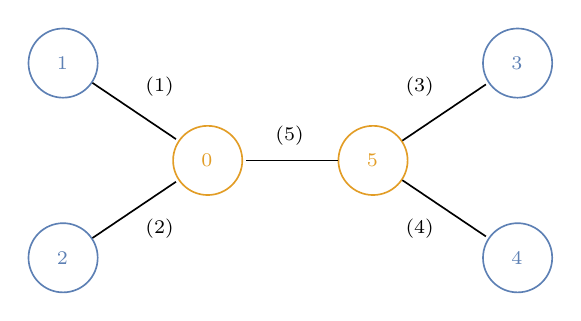
\begin{tikzpicture}[->,>=stealth',shorten >=1pt,auto,node distance=0.6cm and 1.2cm,semithick]
	\tikzstyle{every state}=[]

	\node[state] (1) [BLUE] {$\state_1$};
	\node[state] (0) [YELLOW, below right=of 1] {$\state_0$};
	\node[state] (2) [BLUE,below left=of 0] {$\state_2$};
	\node[state] (5) [YELLOW,right=of 0] {$\state_5$};
	\node[state] (3) [BLUE,above right=of 5] {$\state_3$};
	\node[state] (4) [BLUE,below right=of 5] {$\state_4$};

	\path[-]
	(1) edge [black] node [above right] {$\branchlength^{(1)}$} (0)
	(2) edge [black] node [below right] {$\branchlength^{(2)}$} (0)
	(5) edge [black] node [above] {$\branchlength^{(5)}$} (0)
	(5) edge [black] node [above left] {$\branchlength^{(3)}$} (3)
	(5) edge [black] node [below left] {$\branchlength^{(4)}$} (4);
	\end{tikzpicture}
	\caption[Illustrative phylogenetic tree]{
	Illustrative phylogenetic tree. Internal nodes ($\state_0$ and $\state_5$) are represented in yellow, while extant nodes ($\state_1$ to $\state_4$) for which the state is know from the observed data is represented in blue. The node $0$ is considered the root of the tree, although defining is not strictly required since the process is reversible.}
	\label{fig:tree}%
\end{figure}

In the example of the illustrated tree, from the observed data for the extant nodes $\Data\siteexp = \{ \state_1,\state_2, \state_3, \state_4 \}$, at site $\site$, the \gls{likelihood} given that the states of the internal nodes are known is computed as:
\begin{align}
	p\left(\Data\siteexp| \state_0, \state_5, \Submatrix\siteexp, \branchlength\branchexp, \forall \branch \right) & = \Probmatrix\siteexp_{\state_0, \state_1}(\branchlength^{(1)})
	\Probmatrix\siteexp_{\state_0, \state_2}(\branchlength^{(2)}) \\
	& \quad \quad \quad
	\times \Probmatrix\siteexp_{\state_5, \state_3}(\branchlength^{(3)})
	\Probmatrix\siteexp_{\state_5, \state_4}(\branchlength^{(4)})
	\Probmatrix\siteexp_{\state_0, \state_5}(\branchlength^{(5)}) \notag
\end{align}
In the general topology, $\Data\siteexp = \{ \state_P \hdots \state_{2P-1} \}$, where $\state_{\nodeUp}$ and $\state_{\nodeDown}$ are used to denoted the respectively the parent and descendant nodes of a branch, the \gls{likelihood} of the observed data is given as:
\begin{align}
p\left(\Data\siteexp| \state_{I}, \Submatrix\siteexp, \branchlength\branchexp, \forall (I, \branch) \right) & = \prod_{b} \Probmatrix\siteexp_{\state_{\nodeDown}, \state_{\nodeUp}}(\branchlength^{(\branch)}),
\end{align}
where $I$ runs over all the internal nodes.

Because the states of the internal nodes are not actually unknown, the \gls{likelihood} must be summed over the all the possible states, weighted by their equilibrium stationary frequencies ($\pi\siteexp$).

In the case of the illustrative example, the total probability is given as
\begin{align}
	p\left(\Data\siteexp| \Submatrix\siteexp, \branchlength\branchexp , \forall \branch \right) & = \sum\limits_{\state_0=1}^{61} \subequi_{\state_0} \sum\limits_{\state_5=1}^{61} \subequi_{\state_5} p\left(\Data\siteexp| \state_0, \state_5, \Submatrix\siteexp, \branchlength\branchexp \right) \\
	& = \sum\limits_{\state_0=1}^{61} \subequi_{\state_0} \sum\limits_{\state_5}^{61} \subequi_{\state_5} \Probmatrix\siteexp_{\state_0, \state_1}(\branchlength^{(1)})
	\Probmatrix\siteexp_{\state_0, \state_2}(\branchlength^{(2)}) \\
	& \qquad \qquad \qquad
	\times \Probmatrix\siteexp_{\state_5, \state_3}(\branchlength^{(3)})
	\Probmatrix\siteexp_{\state_5, \state_4}(\branchlength^{(4)})
	\Probmatrix\siteexp_{\state_0, \state_5}(\branchlength^{(5)})\notag
\end{align}

And because the process is reversible, the equilibrium frequencies of \glspl{codon} satisfies the equations:
\begin{align}
\bm{0} & = \bm{\pi}\branchsiteexp \Submatrix\branchsiteexp \\
\iff \bm{\pi}\branchsiteexp & = \bm{\pi}\branchsiteexp \Probmatrix\branchsiteexp \\
\iff \dfrac{\subequi_{\ci}\siteexp}{\subequi_{\cj}\siteexp} & = \dfrac{\submatrix_{\cj, \ci}\siteexp}{\submatrix_{\ci, \cj}\siteexp}
\end{align}

In the general topology, the \gls{likelihood} of the observed data is thus given as:
\begin{align}
p\left(\Data\siteexp| \Submatrix\siteexp, \branchlength\branchexp, \forall \branch \right) & = p\left(\Data\siteexp| \state_{I}, \Submatrix\siteexp, \branchlength\branchexp, \forall (I, \branch) \right), \\
& = \sum\limits_{\state_{0}=1}^{61} \subequi_{\state_{0}} \hdots \sum\limits_{\state_{k}=1}^{61} \subequi_{\state_{k}} \prod_{b} \Probmatrix\siteexp_{\state_{\branch^{+}}, \state_{\branch^{-}}}(\branchlength^{(\branch)}), \label{eq:likelihood-site}
\end{align}

And finally, the assumption of independence between sites allows the probability of an observed set of aligned sequences at the tips of an evolutionary tree to be expressed as the product over alignment columns of the observed nucleotides or amino acids in those columns:
\begin{align}
p\left(\Data| \Submatrix\siteexp, \branchlength\branchexp, \forall (\site, \branch) \right) & = \prod_{\site} p\left(\Data\siteexp| \Submatrix\siteexp, \branchlength\branchexp, \forall \branch \right) \label{eq:likelihood}
\end{align} 
\subsection{Pruning algorithm}
The \gls{likelihood} of observed data at a specific column of a multiple sequence alignment, given by equation \ref{eq:likelihood} requires extensive computation, but can however can be determined with the pruning algorithm of \citet{Felsenstein1985}. 
The \gls{likelihood} of the data $\Data$ can be computed using the pruning algorithm:
\begin{align}
p\left(\Data\siteexp| \Submatrix\siteexp, \branchlength\branchexp, \forall \branch \right) & = \sum\limits_{\ci=1}^{61} \subequi\siteexp_{\ci} \pruning\siteexp_{0} \left( \ci \right)
\end{align}
where $\pruning_{\node} \left( \ci \right)$ is computed recursively from the $2$ descendant children $\node_{1}$ and $\node_{2}$ of an internal node $\node$:
\begin{align}
\pruning\siteexp_{\node} \left( \ci \right) = 
\left[ \sum\limits_{\cj=1}^{61}\Probmatrix\siteexp_{\itoj}(\branchlength^{(\node \to \node_{1})}) \pruning\siteexp_{\node_{1}} \left( \cj \right) \right]
\cdot 
\left[ \sum\limits_{\cj=1}^{61}\Probmatrix\siteexp_{\itoj}(\branchlength^{(\node \to \node_{2})}) \pruning\siteexp_{\node_{2}} \left( \cj \right) \right]
\end{align}
And if the node $\node$ is a node with no descendant, meaning an extant taxa:
\begin{align}
\pruning\siteexp_{\node} \left( \ci \right) =
\begin{dcases}
1, & \text{if } \state_{\node} = \ci \\
0, & \text{otherwise.}
\end{dcases}
\end{align}

\section{Bayesian estimation}
\label{sec-intro:bayesian}

The Bayesian Paradigm can be seen as a way to model uncertainty in a probabilistic way.
In other words, parameter of the models denoted $\theta$ are considered as random variables whose distribution describes that uncertainty.
This unconditional distribution of parameters, $p(\theta)$, is called the \gls{prior}.
The probability of those parameters are going to be modified after acquisition of information supplied by observed data.

$\bullet$ Why has Bayesian statistics been used in phylogenetic inference \citep{Lartillot2020}.

Knowingly that maximum \gls{likelihood} and Bayesian statistics are often opposed to each others and sometimes fiercely defended by their tenant, using one of them implicitly put someone in the position to argument their choice.
Firstly, Bayesian statistics technically is not required to devise procedure necessary to evades local optimums.
Second and most importantly, Bayesian statistics output not a single statistic but a confidence interval, meaning how much certainty is available given the data.
Posterior and \gls{prior} can be thus presented next to each others and differences between the two is due to signal extracted from the data.
A corollary is that over parametrization is not such a drastic issue as in maximum \gls{likelihood} inference, since in a case where there is only limited extractable signal from the data this will reflect in the confidence interval.
In the worst possible case of over-parametrization, namely that of confounded parameters, such that the model is exactly the same for different set of parameters, the confidence interval will expand but confounded parameters can be identified afterward through parameters correlation in their joint \gls{posterior} distribution.
The subjective arbitrary introduced by lasso and penalized-likelihood is replaced by statistical \gls{prior} distribution.
However, over-parameterized models is still a misappropriate use of computing resource, which results in a greater environmental cost.

Formally, Bayes theorem is essential in updating of the distribution :
\begin{equation}
	p(\theta|\data)=\frac{p(\data|\theta)p(\theta)}{p(\data)}
\end{equation}
The probability of the parameters matrix $\theta$ given the data is called the \gls{posterior} probability, it is \gls{posterior} to the data, and $p(\data|\Probmatrix)$ is the 

Because the actual probability of the data is not going to change, in inference Bayes theorem is often presented as:
\begin{equation}
p(\data|\data) \propto p(\data|\data)p(\data)
\end{equation}
Simply stating that the \gls{posterior} is proportional to the \gls{likelihood} time the \gls{prior}.

From the \gls{likelihood} of the data derived in the previous section, the difficulties now is shifted to the definition of the \gls{prior} distribution, where these difficulties come in two flavors.
Firstly, the parameters of evolution for which \gls{prior} distribution can be apprehended might be the parameters of interest such as the selection coefficient, or on the mutation rate, but not the \gls{prior} distribution of the \gls{substitution} rate matrix as a whole.
This difficulties is eased by Bayesian network, which are a probabilistic graphical representation of a set of variables and their conditional dependencies via a directed acyclic graph (DAG).
In the example of the \gls{prior} distribution for the rate \gls{substitution} matrix, it is determined as the joint distribution of the \gls{prior} over the selection coefficient and the mutation rate matrix, which itself is given by the joint distribution over the equilibrium frequencies of nucleotides and exchangeabilities rates for the general-time-reversible (GTR) mutation matrix (see figure \ref{fig:DAG}).
Seeing the DAG the other way around (following the arrows), simple \gls{prior} distribution are combined together to form more complex joint \gls{prior} distribution which ultimately define the \gls{prior} distribution of the model ($\theta$).

\begin{figure}[H]
	\centering
	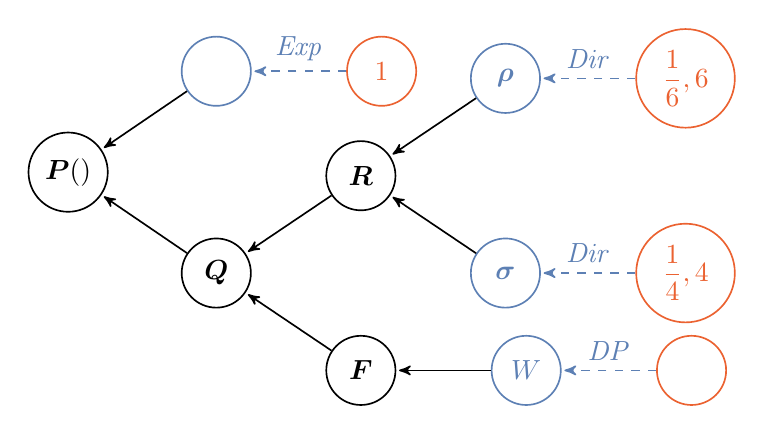
\begin{tikzpicture}[->,>=stealth',shorten >=1pt,auto,node distance=0.6cm and 1.2cm,semithick]
	\tikzstyle{every state}=[]
	
	\node[state] (P) {$\Probmatrix\siteexp(\branchlength\branchexp)$};
	\node[state] (Q) [below right=of P] {$\Submatrix\siteexp$};
	\node[state] (BL) [BLUE, above right=of P] {$\branchlength\branchexp$};
	\node[state] (Exp) [RED, right=of BL] {$1$};
	\node[state] (F) [below right=of Q] {$\bm{F}\siteexp$};
	\node[state] (sb) [BLUE, right=of F] {$W$};
	\node[state] (sbH) [RED, right=of sb] {$\stickbreakinghyper$};
	\node[state] (R) [above right=of Q] {$\Mutmatrix$};
	\node[state] (Ex) [BLUE, above right=of R] {$\Exchan$};
	\node[state] (ExH) [RED, right=of Ex] {$\dfrac{1}{6}, 6$};
	\node[state] (Equi) [BLUE, below right=of R] {$\Mutequi$};
	\node[state] (EquiH) [RED, right=of Equi] {$\dfrac{1}{4}, 4$};
	
	\path 
	(Q) edge [black] node [above right] {} (P)
	(BL) edge [black] node [] {} (P)
	(Exp) edge [dashed, BLUE] node [above] {\textit{Exp}} (BL)
	(R) edge [black] node {} (Q)
	(Ex) edge [black] node [] {} (R)
	(Equi) edge [black] node [below] {} (R)
	(ExH) edge [dashed, BLUE] node [above] {\textit{Dir}} (Ex)
	(EquiH) edge [dashed, BLUE] node [above] {\textit{Dir}} (Equi)
	(F) edge [black] node {} (Q)
	(sb) edge [black] node [above] {} (F)
	(sbH) edge [dashed, BLUE] node [above] {\textit{DP}} (sb);
	\end{tikzpicture}
	\caption[Directed acyclic graph of Bayesian network]{
	Directed acyclic graph of dependencies between variables.
	Nodes of the directed acyclic graph are the variables, and edges are the functions. Hyper-parameters are depicted in {\color{RED}{red}} circle, random variables in {\color{BLUE}{blue}} circles, and transformed variables in black.
	{\color{BLUE}{blue}} solid line denotes a drawing from a random distribution, and black solid lines denote a function.
	\textit{Exp} denotes an exponential distribution, \textit{Dir} denotes a Dirichlet distribution, and finally \textit{DP} denotes a \gls{Dirichlet-process}.}
	\label{fig:DAG}
\end{figure}

Secondly, once realizing that the \gls{prior} distribution can be boiled to a set of simpler \gls{prior} distributions, the difficulty arise from the high dimensionality of the parameter space, known as the curse of dimensionality.
More precisely, the number of states increases exponentially with the number of dimension of the space, such that the space is too large to be explored and computation of both the \gls{prior} and the \gls{likelihood} for each set of parameters is unrealistic.
Reduction in the exploration of the state space is obtained by employing Monte-Carlo Markov-Chain, which effectively approximate the target \gls{posterior} distribution.

\subsection{Monte-Carlo Markov-Chain}

The first \acrshort{MC} algorithm is associated with the army laboratory in Los Alamos under the direction of Metropolis in early 1952.
Both a physicist and a mathematician, Nicolas Metropolis was one of the first scientists to work on the Manhattan Project that led to the production of the atomic bomb.
Almost as early, he became obsessed with the hydrogen bomb, which he eventually succeed in building.

Published in June 1953 in the \textit{Journal of Chemical Physics}, the primary focus of \acrshort{MC} algorithm is computing the energy of random configurations for a system of many particles.
This energy is not not available analytically and requires integration across for all realizations of the random configurations of the particle system.
Because the number of dimensions is high (twice the number of particles), numerical integration is impossible using a deterministic algorithm.
Moreover, because the probability of a given configuration can be very small, even Monte Carlo integration, by sampling randomly across the target distribution of configurations fails to correctly approximate this integral.

This problem can however be transposed in the \gls{mc} realm, where each state of the process is a particular configuration of particles.
The {transition} probabilities between states must generate a stationary distribution equal to the target distribution of particle configurations.
Given this requirement, and given we can also sample from the {transition} probabilities, the Monte Carlo \gls{mc} starts from a given state and can be updated by random sampling from the {transition} probabilities.
The chain is composed of a period of burn-in, where the current state is of low probability relative to more likely states.
Once reaching the dynamic equilibrium, the energy of each configuration can be computed and the average of this energy is an approximate solution for the integral of energy over the distribution of configurations.

\subsection{Metropolis-Hastings sampling}

The Metropolis algorithm is an acceptance/rejection rule for the probabilities of {transition} allowing to match the stationary distribution to the specified target distribution, present in the original paper.
From a state $X_t$, the algorithm proceeds as follows at each step of the \gls{mc}:
\begin{itemize}
	\item Generate a random candidate state $X'$ according to $g(X'\mid X_t)$.
	\item Calculate the acceptance ratio $\displaystyle r=\min \left(1,{\frac {P(X')}{P(X_{t})}}{\frac {g(X_{t}\mid X')}{g(X'\mid X_{t})}}\right)$.
	\item Generate a uniform random number $u\in [0,1]$.
	If $u\leq A(X',X_{t})$, then accept the new state and set $X_{t+1}=X'$.
	Else reject the new state and set $X_{t+1}=X$
\end{itemize}

The algorithm requires the ability to calculate the acceptance ratio $r$ for all possible jump, and to draw a jump from any state. 
In addition, last step above requires the generation of a uniform random number.
The Metropolis procedure has been developped in the context of a symmetric distribution $g(X'\mid X) = g(X \mid X')$, and was later generalized to incorporate any distribution, such that the factor $g(X'\mid X) / g(X \mid X')$ took the name Hasting ratio.

\subsection{Gibbs sampling}

Gibbs sampling is applicable when a joint distribution of variables is not known explicitly or is difficult to sample from directly, but the conditional distribution of each variable are easier to sample from.
The original implementation of the Gibbs sampler was applied to a discrete image processing problem, a problem somewhat removed from statistical inference in the classical sense.
This paper is also responsible for the name {\it Gibbs sampling}, because it implemented this method for the Bayesian study of {\it Gibbs random fields} which, in turn, derive their name from the physicist Josiah Willard Gibbs (1839-1903).

The individual variables are sampled one at a time, with each variable conditioned on the most recent values of all the others.
It can be shown that the sequence of samples constitutes a \gls{mc}, and the stationary distribution of that \gls{mc} is just the joint distribution.
Gibbs sampling is particularly well-adapted to sampling the \gls{posterior} distribution of a Bayesian network, since they are composed of a set of individual random variables in which each variable is conditioned on only a small number of other variables.

Gibbs sampling can be considered a general framework for sampling from a large set of variables by sampling each variable (or in some cases, each group of variables) in turn.
Various algorithms can be used to sample these individual variables, depending on the exact form of the multivariate distribution, it can incorporate the Metropolis–Hastings algorithm, or more sophisticated methods such as slice sampling, adaptive rejection sampling and adaptive rejection Metropolis.

\subsection{Sufficient statistics \& data augmentation}

The basic idea is to augment the observed sequence data with a possible \gls{substitution} history and to then use \gls{mc} Monte Carlo techniques to perform a random walk over histories that are consistent with the observed data.

A realization of the random process results in a detailed \gls{substitution} history over the tree.
Most phylogenetic Monte-Carlo-Markov-Chain (\acrshort{MC}) samplers target the distribution over the model parameters, which means that they have to repeatedly invoke the pruning algorithm to recalculate
the pruning-based \gls{likelihood} which is most often the limiting step of the \acrshort{MC}.

An alternative, which is used here, is to do the \acrshort{MC} conditionally on the detailed \gls{substitution} history $\subhistory$, thus doing the \acrshort{MC} over the augmented configuration~($\subhistory$, $\data$), under the target distribution obtained by combining the mapping-based \gls{likelihood} with the \gls{prior} over model parameters

The key idea that makes this strategy efficient is that the mapping-based \gls{likelihood} depends on
compact summary statistics of $\subhistory$ (which in turn depend on the specific parameter component
being resampled), leading to very fast evaluation of the \gls{likelihood}.
On the other hand, this requires to implement more complex \acrshort{MC} procedures, that have to alternate between:

1) sampling $\subhistory$ conditionally on the data and the current parameter configuration.

2) re-sampling the parameters conditionally on $\subhistory$.

To implement the mapping-based \acrshort{MC} sampling strategy, we first sample the detailed \gls{substitution} history $\subhistory$ for all sites along the tree.
Several methods exist for doing this~\citep{Nielsen2002,Rodrigue2008}.
Then, we write down the probability of $\subhistory$ given the parameters, and finally, we collect all factors that depend on some parameter of interest and make some simplifications.
This ultimately leads to relatively compact sufficient statistics (Supplementary Materials for the different sufficient statistics used by our model) that are fast to evaluate~\citep{Irvahn2014,Davydov2016}.

\subsection{Implementation}

$\bullet$ The work developped in this manuscript

$\bullet$ Modularity of the code, JAGS, MrBayes, RevBayes and now BayesCode,
\url{https://github.com/bayesiancook/bayescode}
\chapter{Thesis objectives}
{\hypersetup{linkcolor=GREYDARK}\minitoc}
\label{chap:goals}

The neutral theory, and its nearly-neutral extension, such as historically reviewed in chapter~\ref{chap:intro-historical}, have deeply influenced our understanding of population genetics and molecular evolution.
Beyond the disputes and the controversies between neutralism and selectionism, the current consensus is to view the evolution of genetic sequences as a stochastic process.
One component of this process is creating diversity through mutation, another antagonistic component is filtering out this diversity through selection, and finally the balance between these components is tuned by effective population size, which determines the amount of random drift, formally presented in chapter~\ref{chap:intro-formalism}.
The long-term outcome of this evolutionary process is an accumulation of point substitutions (both synonymous and non-synonymous) between species.
Relying on this primary source of information contained in multiple sequence alignments of protein-coding genes obtained from contemporaneous species, the aim of phylogenetic codon models, as discussed in chapter~\ref{chap:intro-codon-models}, is to better characterize and quantify the interplay between mutation, selection and random drift.
Codon models are still an active area of research, and proceed from two different philosophies.
On one side, phenomenological models, aiming to capture the net effect of selection through $\omega = \dnds$.
On the other side, mechanistic approaches, with the more ambitious aim of modelling the fine-grained fitness landscape.
As it stands, however, many questions are still open, and current models, whether phenomenological or mechanistic, present many weaknesses.
Phenomenological approaches could still be improved, while staying in the idea of not explicitly modelling the detailed fitness landscape.
As for mechanistic approaches, in their current versions, they are making very strong assumptions, such as site independence, a time-independent fitness landscape, but also constant effective population size across the whole phylogeny.
More fundamentally, there is a certain gap to be filled between these two alternative approaches, and better connections could be made between them.

In this context, my thesis work represents an attempt at revisiting the question of how to correctly disentangle the complex interactions between mutation, selection and random drift using phylogenetic codon models, under both approaches, either phenomenological or mechanistic.
During this work, I have confronted theoretical insights with empirical data, using a combination of analytical developments, simulation experiments and Bayesian inference.
The results are divided in three chapters, each written in the form of an independent manuscript that shall be submitted to peer-reviewed journals.
The first article (chapter~\ref{chap:NucleotideBias}) revisits the question of the balance between mutation bias and selection, and how this balance should be properly formalized in the context of classical (phenomenological) codon models.
The second manuscript (chapter~\ref{chap:MutSelDrift}, with supplementary materials in chapter~\ref{chap:MutSelDrift-SuppMat}) explores the question of accounting for the variation in long-term effective population size ($\Ne$) between species, in the context of a mechanistic mutation-selection model.
The work presented in this manuscript represents the most intensive part of the PhD work, in terms of modelling, Monte-Carlo algorithmic (see chapter~\ref{chap:intro-inference}) and software development.
Finally, some of the observations made during this second part of my work, in particular the relatively narrow dynamic range of variation in $\Ne$ uncovered using this fully mechanistic approach, have prompted me to revisit the question of how protein biophysics (see chapter~\ref{chap:intro-physic-proteins}), and more generally epistasis, can quantitatively modulate the response of the molecular evolutionary process to changes in effective population size.
This last work is presented as a third manuscript (chapter~\ref{chap:GenoPhenoFit}, with supplementary materials in chapter~\ref{chap:GenoPhenoFit-SuppMat}).

\section{Robustness of codon models to mutational bias}
\label{sec-goals:NucleotideBias}

Nucleotide composition in protein-coding sequences is the result of the equilibrium between mutation and selection.
Because of selection, the nucleotide composition of protein-coding sequences is different from what would be expected under a pure mutational process.
In particular, it differs between the three coding positions, with the third position showing more extreme composition than the first and the second positions.
This empirical observation is well known.
Yet, classical codon models (see chapter~\ref{chap:intro-codon-models}) do not correctly capture this phenomenon.
Instead, in their classical parameterization, in terms of a 4x4 nucleotide rate matrix and a single $\omega$ parameter, phenomenological codon models predict that the nucleotide composition should be the same for all $3$ positions of the codons, and should be equal to the equilibrium frequencies of the underlying 4x4 nucleotide process.
Alternatively, to accommodate this variation across coding positions, some models allow for different nucleotide rate matrices at the three positions.
However, this approach is problematic since the mutation process should in principle be blind to the coding structure, and should be homogeneous across coding positions.
Although this misconception has probably minor impact on the detection of positive selection, it is a clear symptom of a more fundamental issue with teasing apart mutation rates and fixation biases in the context of phenomenological codon models.
Practically, this could have important consequences, in particular, given the current interest in modelling the impact of GC-biased gene conversion (\acrshort{gBGC}) on the evolution of protein-coding sequences, a factor which requires mutation and fixation biases to be carefully disentangled.
Conceptually, the problem comes from the fact that, at the mutation-selection equilibrium, there is net selection differential, or net fixation bias, acting against the mutational pressure.
In other words, at equilibrium, $\omega$ is not the same in different mutational directions.
Because they capture selection through a single parameter $\omega$, classical codon models cannot correctly capture this net fixation bias.
To address this problem, chapter~\ref{chap:GenoPhenoFit} presents an alternative modelling approach, where $\omega$ is not anymore seen as a scalar, but as an array of $\omega$ values unfolding along multiple directions.
This model is tested against empirical and simulated protein coding \acrshort{DNA} alignment.

\section{Inferring long-term population size}
\label{sec-goals:MutSelDrift}

Presented in section~\ref{sec:intro-classical-codon-models}, mechanistic phylogenetic codon models are grounded on population genetics first principles.
Being explicitly parameterized in terms of mutation rates and population-scaled fitness coefficients, these models represent a principled approach for investigating the intricate interplay between mutation, selection and drift.
In their current form, mutation-selection models assume a fixed and site-specific fitness landscape, without epistasis.
As a result, they are entirely characterized by the collection of site-specific amino-acid fitness profiles.
However, thus far, they have relied on the assumption of a constant effective population size across the phylogeny, clearly an unreasonable hypothesis.
Selection and drift are confounded parameters, but they can nevertheless be disentangled by assuming that fitness is fixed along the phylogeny but changing along the sequence, and orthogonally, by assuming that effective population size is constant across sites, but variable across the phylogeny.
In addition to effective population size ($\Ne$), the mutation rate ($\mu$) is also susceptible to vary between lineages.
Furthermore, both $\Ne$ and $\mu$ are expected to co-vary with life-history traits (\acrshort{LHT}).
This suggests that the model should more globally account for the joint evolutionary process followed by all of these lineage-specific variables (Ne, $\mu$, and LHT).
In this direction, chapter~\ref{chap:MutSelDrift} introduces an extended mutation-selection model jointly reconstructing the fitness landscape across sites and long-term trends in effective population size, mutation rate and life-history traits along the phylogeny, from an alignment of \acrshort{DNA} coding sequences and a matrix of observed life-history traits in extant species.
The model was implemented in a Bayesian Monte Carlo framework (see chapter~\ref{sec:intro-bayesian}).
Together, the model estimates correlation between reconstructed life-history traits, mutation rate and effective population size, intrinsically including phylogenetic inertia.
It was tested against simulated data, and finally applied to empirical data in mammals, isopods, primates and drosophila.
The reconstructed history of $\Ne$ in these groups appears to correlate with life-history traits or ecological variables in a way that suggests that the reconstruction is reasonable, at least in its global trends.
On the other hand, the range of variation in $\Ne$ inferred across species is surprisingly narrow.
This last point suggests that some of the assumptions of the model, in particular concerning the structure of the assumed fitness landscape, are potentially problematic.

\section{Substitution rate response to changes in effective population size and expression level}
\label{sec-goals:GenoPhenoFit}

The surprisingly narrow range of variation in $\Ne$ inferred across large phylogenies by the mechanistic mutation-selection model such as mentioned above (section~\ref{sec-goals:MutSelDrift}), prompted me to conduct a more detailed theoretical investigation of the quantitative impact of changes in $\Ne$ on the molecular evolutionary process followed by protein-coding sequences.
A particularly important variable to investigate in this direction is the substitution rate of selected mutations relative to the neutral substitution rate $\omega = \dnds$.
Under the nearly-neutral theory of evolution, lineages with large effective population size ($\Ne$) are expected to undergo stronger purifying selection, and consequently a decrease in $\omega$.
Empirical correlation patterns between $\omega$ and either life-history traits or synonymous diversity (which is a proxy of $\Ne$), have tended to confirm this prediction.
However, simulations using computational models based on the biophysics of protein conformational stability (presented in section~\ref{sec:intro-protein-biophysics}) have suggested that $\omega$ can in fact be virtually independent of $\Ne$.
The discrepancy between these conclusions suggests that a more detailed quantitative investigation of what determines the quantitative response of $\omega$ to changes in $\Ne$, depending on the exact model of the mapping from sequences to fitness, would be useful.
Another related question is how $\omega$ varies between proteins, depending on their expression level.
Empirically, there is a robust negative correlation between $\omega$ and expression level across genes.
Theoretically, many biophysically inspired models suggest that the response of $\omega$ to changes in expression levels should be the same as, or similar to, its response to changes in $\Ne$.
This suggests that the two questions, the impact of changes in $\Ne$ and in expression levels, would benefit from a simultaneous theoretical investigation.
To address these questions, chapter~\ref{chap:GenoPhenoFit} derives a theoretical approximation for the quantitative response of $\omega$ to changes in $\Ne$ and in expression level, under an explicit genotype-phenotype-fitness map.
The method presented is generally valid for an additive trait and log-concave fitness functions, but more specifically applied to protein undergoing selection for their conformational stability.
The analytical results, obtained under simplified models, are corroborated by simulations under more complex models.
Finally, analytical predictions of $\omega$ response to changes in $\Ne$ and expression level are confronted to empirical data, while other aspects of protein biophysics such as protein-protein interactions are also discussed.

\begin{figure}[htbp]
	\centering
	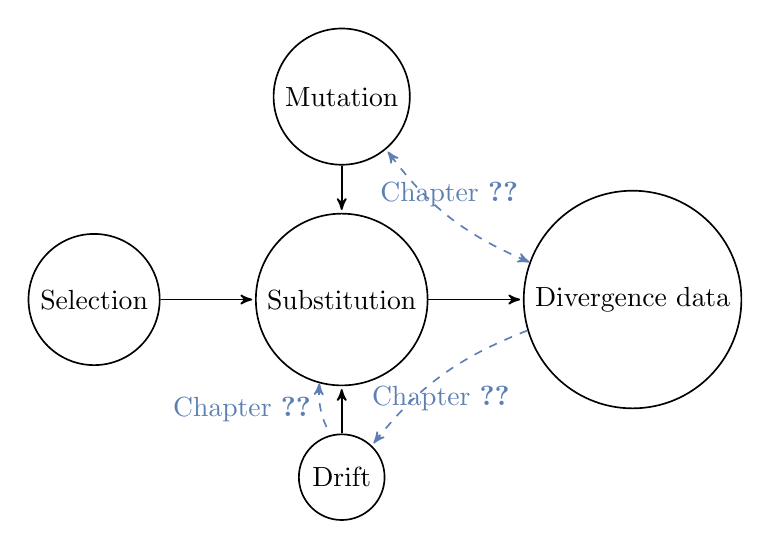
\begin{tikzpicture}[->,>=stealth',shorten >=1pt,auto,node distance=0.6cm and 1.2cm,semithick]
		\tikzstyle{every state}=[]

		\node[state] (0) {Substitution};
		\node[state] (mut) [above=of 0] {Mutation};
		\node[state] (sel) [left=of 0] {Selection};
		\node[state] (drift) [below=of 0] {Drift};
		\node[state] (sub) [right=of 0] {Divergence data};

		\path[]
		(mut) edge [black] node [above right] {} (0)
		(sub) edge [<->, BLUE, bend left=15, dashed] node [above] {Chapter~\ref{chap:NucleotideBias}} (mut)
		(sel) edge [black] node [below right] {} (0)
		(sub) edge [->, BLUE, bend right=15, dashed] node [below] {Chapter~\ref{chap:MutSelDrift}} (drift)
		(0) edge [black] node [above left] {} (sub)
		(0) edge [<-, BLUE, bend right=15, dashed] node [left] {Chapter~\ref{chap:GenoPhenoFit}} (drift)
		(drift) edge [black] node [above] {} (0);
	\end{tikzpicture}
	\caption[Goal of the thesis]{
	In this thesis, several aspects of the mutation, selection and drift equilibrium are studied and related to empirical data, in the context of protein-coding \acrshort{DNA} sequences.
	Firstly, because the composition of protein-coding \acrshort{DNA} sequences does not reflect the underlying mutational process, but its filtering by selection at the level of amino acids, a careful phenomenological modelling is necessary to uncover mutational process and nucleotide fixation bias, a study presented in chapter~\ref{chap:NucleotideBias}.
	Secondly, the balance between mutation and selection is arbitrated by drift, which is mediated by effective population size and its changes along a phylogeny can be estimated by mechanistic codon models, a study presented in chapter~\ref{chap:MutSelDrift}.
	Finally, selection for protein stability implies an analytical relationship between the rate of evolution and effective population size and protein expression level, a study presented in chapter~\ref{chap:GenoPhenoFit}.
	}
	\label{fig:goals}
\end{figure}


\part{Results}
\label{part:results}
\chapter{Robustness of codon models to mutational bias.}
\minitoc
\section{Abstract}

Protein-coding sequences subjected to mutational bias at the nucleotide level, and evolving under selection at the amino-acids will lean toward lower mutational bias when observed at the protein level. Unfortunately, parametric codon models developed to estimate the rate of evolution on amino-acids use the observed mutational bias at the protein level and don't take into account this effect. Thus, such parametric codon models are inherently misspecified to untangle mutation and selection, and they don't estimate the mutational process reliably. We also show that even if the mutational process is misspecified, parametric codon models are able to estimate reliably the rate of evolution acting on amino-acids. But if one wants to also estimate the mutational process, one need to use model where the rate of evolution is a tensor (95 parameters) instead of a single parameter.

\section{Notations}

\begin{itemize}
	\item $\Ne \in \mathbb{N}$ is the effective population size.
	\item $t \in \mathbb{R}_{\geq 0}$ is the time measured in unit of population size ($t=1 \Rightarrow 4 \Ne $ generations).
\end{itemize}

\subsection{\acrshort{DNA}}
\begin{itemize}
	\item $\mu \in \mathbb{R}_{\geq 0}$ is the \acrshort{DNA} mutation rate for one site of the sequence in one generation.
	\item $\theta=4 \Ne \mu \in \mathbb{R}_{>0} $ is the scaled mutation rate.
	\item $ \SetWeak = \left\{ A,T \right\} $ is the set of $2$ weak nucleotides ($2$ hydrogen bonds).
	\item $ \SetStrong = \left\{C,G \right\} $ is the set of $2$ strong nucleotides ($3$ hydrogen bonds).
	\item $\lambda \in \mathbb{R}_{\geq 0} $ is the relative rate of weak over strong mutations.
	\item $ \SetNuc = \SetWeak \cup \SetStrong =\left\{ A,C,G,T \right\} $ is the set of $4$ nucleotides in lexicographic order.
	\item $a \in \SetNuc $ and $b \in \SetNuc $ are used to denote nucleotides.
	\item $u_{a,b} \in \mathbb{R}_{> 0}$ is the mutation rate from nucleotide $a$ to $b$.
	\item $\bm{u} \in \mathbb{R}_{> 0}^{4 \times 4} $ is the mutation rate matrix between nucleotides.
	\item $\pi_a \in \left]0,1\right[ $ is the stationary distribution of nucleotide $a$. $\sum_{a \in \Omega_{\mathrm{Nuc}}} \pi_a = 1$.
	\item $\pi = \left(\pi_A , \pi_C , \pi_G , \pi_T \right) \in \left]0,1\right[^4$ is the vector of nucleotides stationary distribution.
\end{itemize}

\subsection{Codons}
\begin{itemize}
	\item $\SetCodon = \left\{ AAA,AAC, \dots, TTT \right\} $ is the set of $61$ non-stop codons in lexicographic order.
	\\By definition $\SetCodon = \left\{ \SetNuc \times \SetNuc \times \SetNuc \right\} \setminus \left\{ TAA, TAG, TGA \right\} $.
	\item $x \in \SetCodon $, $y \in \SetCodon $ and $y \in \SetCodon $ are used to denote the codons.
	\item $\NxAB \subset \SetCodon $ is the set of neighboring codons to codon $x$ such that the mutation is from nucleotide in $A \in \left\{ \SetWeak, \SetStrong \right\}$ to nucleotide in $B \in \left\{ \SetWeak, \SetStrong \right\}$.
	\item $\Nx =  \NxSS \cup \NxSW \cup \NxWS \cup \NxWW \subset \SetCodon $ is the set of neighboring codons to codon $x$.
	\item $w_x \in \left\{0,1,2,3 \right\}$ is the number of weak bases ($A$ and $T$) of codon $x$.
	\\For example $x=ACT \Rightarrow w_x=2$, or  $x=ACA \Rightarrow w_x=2$, or $x=ACG \Rightarrow w_x=1$.
	\item $U_{x,y} \in \mathbb{R}_{\geq 0} $ is the mutation rate from codon $x$ to $y$.
	\item $n \in \mathbb{N}$ is the number of codon sites in the sequence.
	\item $k \in \left\{ k \in \mathbb{N} \mid 1 \leq k \leq n \right\}$ is the $k^{\mathrm{th}}$ codon site of the sequence.
	\item $Q_{x,y}^{(k)} \in \mathbb{R}_{\geq 0} $ is the substitution rate from codon $x$ to $y$ at site $k$.
	\item $\bm{Q}^{(k)} \in \mathbb{R}_{\geq 0}^{61 \times 61} $ is the substitution rate matrix of codons at site $k$.
	\item $\Pi_x^{(k)} \in \left]0,1\right[ $ is the stationary distribution of codon $x$ at site $k$. $\sum_{x \in \SetCodon} \Pi_x^{(k)} = 1$.
	\item $\Pi^{(k)} = \left( \Pi_x , \ \forall x \in \SetCodon \right) \in \left]0,1\right[^{61} $ is the vector of codon stationary distribution.
\end{itemize}

\subsection{Amino-acids}
\begin{itemize}
	\item $\SetAa = \left\{ \mathrm{Arginine}, \dots ,\mathrm{Tyrosine} \right\} $ is the set of 20 amino-acids in lexicographic order.
	\item $X \in \SetAa $, $Y \in \SetAa$ and $Y \in \SetAa$ are used to denote the amino-acid encoded by codon $x$ and $y$.
	\\For example $x=ACT \Rightarrow X=$ Threonine.
	\item $\NxNonSyn \subset \Nx $ is the set of non-synonymous neighboring codons of codon $x$.
	\\By definition $\NxNonSyn = \left\{ y \in \Nx  \mid \ Y \neq X  \right\} $.
	\item $\NxSyn \subset \Nx $ is the set of synonymous neighboring codons of codon $x$.
	\\By definition $\NxSyn = \left\{ y \in \Nx \mid \ Y = X  \right\} $ and $\NxSyn \cup \NxNonSyn = \Nx $.
	\item $F_X^{(k)} \in \mathbb{R} $ is the fitness of amino-acid $X$, and thus of codon $x$ at site $k$.\\
	The fitness are normalized such that $\sum_{X \in \SetAa}\e^{F_X^{(k)}} = 1 $
	\item $F^{(k)} = \left( F_X , \ \forall X \in \SetAa \right) \in \mathbb{R}^{20} $ is the vector of amino-acids fitness at site $k$.
	\item $\bm{F} = \left( F^{(k)} , \  1 \leq k \leq n \right) \in \mathbb{R}^{20 \times n} $ is the matrix of amino-acids fitness for the whole sequence.
\end{itemize}

\subsection{Distribution of fitness effects}
\begin{itemize}
	\item $s_X = \e^{F_X} \in \left]0,1\right[ $ is the propensity of amino-acid $X$.\\
	The propensities are normalized such that $\sum_{X \in \SetAa}s_X = 1 $.
	\item $s = \left( s_X , \forall X \in \SetAa \right) \in \left]0,1\right[^{20} $ is the vector of amino-acids propensities.
	\item $C(s) = \left\{ s \mid \sum_{X \in \SetAa} s_X = 1  \right\} $ is the $19$-dimensional simplex of propensities.
	\item $\forall z \in \mathbb{R}_{>0}, \ \Gamma(z) = \int_{0}^{\infty} x^{z-1} \e^{-x} \der x \in \mathbb{R}_{>0} $ is the gamma function.
	\item $\mathrm{Dirichlet}(\alpha, 20)$ is the Dirichlet distribution of order $20$ with concentration parameter $\alpha \in \mathbb{R}_{>0}$.
	\item $p(z) \in \mathbb{R}_{\geq 0}$ is the probability density function of the continuous random variable $Z$.
	\item $S \sim \mathrm{Dirichlet}(\alpha, 20) \Rightarrow	p(s; \alpha) = {\frac {\Gamma (20 \alpha)}{\Gamma (\alpha )^{20}}} \prod_{X \in \SetAa} s_X^{\alpha-1}, \ \forall s \in C(s)$.
	\item $\operatorname{E}[f(S)] = \int_{C(s)} f(s) p(s; \alpha) \der s$ is the expected value of $f(S)$ for any function $f$.
\end{itemize}

\section{Summary}

The nucleotide frequencies in protein-coding sequences is the result of the equilibrium between mutation and
selection. As a consequence, protein-coding sequences subjected to mutational bias at the nucleotide level,
and evolving under selection at the amino-acids, will lean toward lower mutational bias when observed at
the protein level. Unfortunately, parametric codon models developed to estimate the rate of evolution on
amino-acids use the observed mutational bias at the protein level and don’t take into account this effect.
Thus, such parametric codon models are inherently misspecified to untangle mutation and selection, and
they don’t estimate the mutational process reliably. We also show that even if the mutational process is
misspecified, parametric codon models are able to estimate reliably the rate of evolution acting on amino-
acids. But if one wants to also estimate the mutational process, one need to use model where the rate of
evolution is a tensor (95 parameters) instead of a single parameter.
We seek to simulate the evolution of protein-coding sequences along a specie tree. Starting with one
sequence at the root of the tree, the sequences evolves independently along the different branches of the
tree, until they reach the leaves. At the end of the simulation, we get one sequence for each leaf of the
tree, meaning one sequence per specie. Such evolutionary process is an idealized version of the reality, in
the sens that the whole heterogeneity of sequences in the population is wiped away, with only one sequence
representing the whole population. To make such idealized process more realistic, one can use population-
genetic framework. In population-genetics, a change in the whole population sequence, called substitution,
is modeled as the product of a mutation and a fixation. A mutation only appear in one specific individual of
the population, and a fixation is the probability that this specific individual is eventually a parent of all the
population later in time. One interesting result of population genetic is that the substitution rate is equal to
the mutation rate if the mutations are selectively neutral. If a mutation is favored (disfavored) by selection,
the substitution rate is higher (lower) than the neutral rate.
For a protein-coding \acrshort{DNA} sequence, a substitution is modeled as the product of mutation at the nucleotide
level, and selection of the amino-acid level. On one hand, the mutation rate between nucleotides as assumed
to be same for all sites of the sequences. On the other hand, the selection for amino-acids is not assumed
to be the same for all sites of the sequences. For example, an exterior site (solvent accessible residue) might
favor hydrophilic amino-acids, and an interior site of the protein might favor hydrophobic amino-acids.


\section{Introduction}

We seek to simulate the evolution of protein-coding sequences along a specie tree.
Starting with one sequence at the root of the tree, the sequences evolves independently along the different branches of the tree, until they reach the leaves. At the end of the simulation, we get one sequence for each leaf of the tree, meaning one sequence per specie.
Such evolutionary process is an idealized version of the reality, in the sens that the whole heterogeneity of sequences in the population is wiped away, with only one sequence representing the whole population. To make such idealized process more realistic, one can use population-genetic framework. In population-genetics, a change in the whole population sequence, called substitution, is modeled as the product of a mutation and a fixation. A mutation only appear in one specific individual of the population, and a fixation is the probability that this specific individual is eventually a parent of all the population later in time. One interesting result of population genetic is that the substitution rate is equal to the mutation rate if the mutations are selectively neutral. If a mutation is favored (disfavored) by selection, the substitution rate is higher (lower) than the neutral rate.\\

For a protein-coding DNA sequence, a substitution is modeled as the product of mutation at the nucleotide level, and selection of the amino-acid level. On one hand, the mutation rate between nucleotides as assumed to be same for all sites of the sequences. On the other hand, the selection for amino-acids is not assumed to be the same for all sites of the sequences. For example, an exterior site (solvent accessible residue) might favor hydrophilic amino-acids, and an interior site of the protein might favor hydrophobic amino-acids.

\section{Simulation of protein-coding sequences evolution}

\subsection{Modeling mutational bias}
\label{sec:mutBias}
The mutation rate between nucleotides is always proportional to $\mu$. Moreover, mutations from any nucleotide to another weak nucleotide is increased by the factor $\lambda$ compared with mutations to another strong nucleotides. The rate at which a nucleotide doesn't change is given such the sum of all rates is zero.
\begin{equation}
\label{nucRates}
u_{a, b} =
\begin{dcases}
\mu
& \mathrm{if} \ b \in \SetStrong \ \mathrm{ and } \ a \neq b, \\
\mu \lambda
& \mathrm{if} \ b \in  \SetWeak \ \mathrm{ and } \ a \neq b,  \\
- \sum_{b \in \SetNuc, \ b \neq a }  u_{a, b}
& \mathrm{if} \ a = b.
\end{dcases}
\end{equation}
And the matrix of mutation rates is:
\begin{equation}
\label{nucMatrix}
\bm{u} =
\begin{pmatrix}
{-\mu(2 + \lambda)} & {\mu} & {\mu} & {\mu \lambda} \\
{\mu \lambda} & {-\mu(1 + 2\lambda)} & {\mu} & {\mu \lambda} \\
{\mu \lambda} & {\mu} & {-\mu(1 + 2\lambda)} & {\mu \lambda} \\
{\mu \lambda} & {\mu} & {\mu} & {-\mu(2 + \lambda)}
\end{pmatrix}.
\end{equation}
The stationary distribution $\Pi$ must be annihilated by the mutation matrix $\bm{u}$, which gives the stationary distribution:
\begin{align}
\pi \bm{u}
& =0, \\
\iff \pi
& =\left( \dfrac{\lambda}{2+2\lambda}, \dfrac{1}{2+2\lambda}, \dfrac{1}{2+2\lambda}, \dfrac{\lambda}{2+2\lambda} \right), \\
\iff \pi_a
& = &
\begin{dcases}
\dfrac{1}{2+2\lambda} & \mathrm{if} \ a \in \SetStrong, \\
\dfrac{\lambda}{2+2\lambda} & \mathrm{if} \ a \in  \SetWeak.  \\
\end{dcases}
\label{nucStationarity}
\end{align}
The process is reversible and fulfills detailed balance conditions for any pair of different nucleotides:
\begin{align}
\pi_a u_{a, b}
& = &
\begin{cases}
( 2 + 2 \lambda)^{-1} \mu
& \mathrm{if} \ a \in \SetStrong, \ b \in \SetStrong \ \mathrm{ and } \ a \neq b,\\
( 2 + 2 \lambda)^{-1} \mu \lambda
& \mathrm{if} \ a \in \SetStrong, \ b \in \SetWeak \ \mathrm{ and } \ a \neq b, \\
\lambda  ( 2 + 2 \lambda)^{-1} \mu
& \mathrm{if} \ a \in \SetWeak, \ b \in \SetStrong \ \mathrm{ and } \ a \neq b,\\
\lambda ( 2 + 2 \lambda)^{-1} \mu \lambda
& \mathrm{if} \ a \in \SetWeak, \ b \in \SetWeak \ \mathrm{ and } \ a \neq b, \ \textrm{from eq.}\ \ref{nucRates} \text{ and } \ \ref{nucStationarity},
\end{cases} \\
& =\pi_b u_{b, a} .
\label{nucMutBalance}
\end{align}
It is important to note that ratio of weak over strong nucleotides frequency at stationarity is equal to $\lambda$:
\begin{align}
\label{lambda}
\dfrac{ \pi_A + \pi_T }{ \pi_C + \pi_G }
& =\dfrac{ \lambda ( 2 + 2 \lambda)^{-1} + \lambda ( 2 + 2 \lambda)^{-1}}{ ( 2 + 2 \lambda)^{-1} +  ( 2 + 2 \lambda)^{-1}}, \ \textrm{from eq.}\ \ref{nucStationarity},\\
& =\lambda .
\end{align}

\subsection{Modeling selection at the amino-acid level}
The mutation rate between a pair of codons is given by the underlying mutation rates between nucleotides. However the rate mutation rate is null if the pair of codons differs by more than one nucleotide:
\begin{equation}
\label{codonMutRates}
U_{x, y} =
\begin{cases}
\mu
& \mathrm{if} \ y \in  \NxSS \cup \NxWS \ \mathrm{ and } \ x \neq y, \\
\mu \lambda
& \mathrm{if} \ y \in \NxSW \cup \NxWW   \ \mathrm{ and } \ x \neq y, \\
0
& \mathrm{if} \  y \notin \Nx \ \mathrm{ and } \ x \neq y, \\
- \sum_{y \in \Nx }  U_{x, y} & \mathrm{if} \ x = y.
\end{cases}
\end{equation}
To note, the substitution rate between codons would be equal to the mutation rate of \ref{codonMutRates} if codons are selectively neutral. However, we subsequently take into the selection acting on codon by modeling it at the amino-acid level, where each amino-acid ($X \in \SetAa$ are given a fitness ($F_X$). By modeling fitness at the amino-acid level, we assume that all codons encoding for one particular amino-acid are selectively neutral. In this modeling framework, the genetic code is of particular importance since the number of codons encoding for a particular amino-acid varies greatly. As an example, Tryptophan is encoded by one codon, while Leucine is encoded by 6 codons. Intuitively, this variation makes the mutation bias more effective in codons encoding for many amino-acids since there are many mutations possible that are selectively neutral (same amino-acid). While the other hand, the mutation bias is more constrained if the amino-acid is encoded by a few codons since there is only a few mutations possible that are selectively neutral.\\

To take into account the heterogeneity of selection between different sites of the protein, we assume that each site $k$ of the sequence is evolving under a different fitness landscape ($F_X^{(k)}, \ \forall X \in \SetAa $).
At one particular site, under a static fitness landscape, the substitution rate between codons are given by the product of the mutation rate and the probability of fixation, given by the formula of Kimura (1983) \citep{kimura_neutral_1983}:
\begin{equation}
\label{codonSubRates}
Q_{x, y}^{(k)} =
\begin{dcases}
U_{x, y}
& \mathrm{if} \ y \in \NxSyn \ (y \in \Nx \ \mathrm{and} \ X = Y),  \\
U_{x, y} \dfrac{F_Y^{(k)} - F_X^{(k)}}{1 - \e^{F_X^{(k)} - F_Y^{(k)}}}
& \mathrm{if} \ y \in \NxNonSyn \ (y \in \Nx \ \mathrm{and} \ X \neq Y),  \\
0
& \mathrm{if} \  y \notin \Nx \ \mathrm{ and } \ x \neq y, \\
- \sum_{y \in \Nx }  Q_{x, y}^{(k)}
& \mathrm{if} \ x = y.  \\
\end{dcases}
\end{equation}
The stationary distribution $\Pi$ must be annihilated by the mutation matrix $\bm{Q}$, which gives the stationary distribution at site $k$:
\begin{align}
\Pi^{(k)} \bm{Q}^{(k)}
& =0 ,\\
\iff \Pi_x^{(k)}
& =A^{(k)} \lambda^{w_x} \e^{F_X^{(k)}} ,\ \forall x \in \SetCodon,\\
& \mathrm{ where } \ A^{(k)} = \left( \sum_{y \in \SetCodon} \lambda^{w_y} \e^{F_Y^{(k)}} \right)^{-1}.
\label{codonStationarity}
\end{align}
Interestingly, the mutation process between codons fulfills an equation similar to detailed balance conditions:
\begin{align}
\lambda^{w_x} U_{x, y}
& = &
\begin{cases}
\lambda^{w_x} \mu
& \mathrm{if} \ y \in \NxSS, \\
\lambda^{w_x} \mu \lambda
& \mathrm{if} \ y \in \NxSW, \\
\lambda^{w_x} \mu
& \mathrm{if} \ y \in \NxWS, \\
\lambda^{w_x} \mu \lambda
& \mathrm{if} \ y \in \NxWW, \ \textrm{from eq.}\ \ref{nucRates},
\end{cases} \\
& = &
\begin{cases}
\lambda^{w_y} \mu
& \mathrm{if} \ y \in \NxSS, \\
\lambda^{w_y - 1} \mu \lambda
& \mathrm{if} \ y \in \NxSW, \\
\lambda^{w_y + 1} \mu
& \mathrm{if} \ y \in \NxWS, \\
\lambda^{w_y} \mu \lambda
& \mathrm{if} \ y \in \NxWW, \ \textrm{by definition of} \ w_x \ \text{and} \ w_y,
\end{cases} \\
& = &
\begin{cases}
\lambda^{w_y} \mu
& \mathrm{if} \ y \in \NxSS, \\
\lambda^{w_y} \mu
& \mathrm{if} \ y \in \NxSW, \\
\lambda^{w_y} \mu \lambda
& \mathrm{if} \ y \in \NxWS, \\
\lambda^{w_y} \mu \lambda
& \mathrm{if} \ y \in \NxWW, \ \textrm{by factoring} \ \lambda,
\end{cases} \\
& = &
\begin{cases}
\lambda^{w_y} \mu
& \mathrm{if} \ x \in \NySS, \\
\lambda^{w_y} \mu
& \mathrm{if} \ x \in \NyWS, \\
\lambda^{w_y} \mu \lambda
& \mathrm{if} \ x \in \NySW, \\
\lambda^{w_y} \mu \lambda
& \mathrm{if} \ x \in \NyWW, \ \textrm{since} \ x \in \NxAB \iff y \in \NyBA,
\end{cases} \\
& = &
\lambda^{w_y} U_{y,x}.
\label{codonMutBalance}
\end{align}
Moreover, the substitution process is reversible and fulfills detailed balance conditions at each site $k$:
\begin{align}
\Pi_x^{(k)} Q_{x, y}^{(k)}
& =A^{(k)} \lambda^{w_x} \e^{F_X^{(k)}}
\begin{cases}
U_{x, y}
& \mathrm{if} \ y \in \NxSyn,  \\
U_{x, y} \dfrac{F_Y^{(k)} - F_X^{(k)}}{1 - \e^{F_X^{(k)} - F_Y^{(k)}}}
& \mathrm{if}  \ y \in \NxNonSyn, \ \textrm{from eq.}\ \ref{codonSubRates} \text{ and } \ \ref{codonStationarity},
\end{cases} \\
& =A^{(k)} \lambda^{w_x} U_{x, y}
\begin{cases}
\e^{F_X^{(k)}}
& \mathrm{if} \ y \in \NxSyn,  \\
\dfrac{F_Y^{(k)} - F_X^{(k)}}{ \e^{-F_X^{(k)}}  - \e^{- F_Y^{(k)}} }
& \mathrm{if}  \ y \in \NxNonSyn, \ \textrm{by rearranging},
\end{cases} \\
& =A^{(k)} \lambda^{w_y} U_{y, x}
\begin{cases}
\e^{F_Y^{(k)}}
& \mathrm{if} \ y \in \NxSyn , \\
\e^{F_Y^{(k)}} \dfrac{F_Y^{(k)} - F_X^{(k)}}{ \e^{F_Y^{(k)}-F_X^{(k)}} - 1 }
& \mathrm{if}  \ y \in \NxNonSyn, \ \textrm{from eq.} \ \ref{codonMutBalance}
\end{cases} \\
& =A^{(k)} \lambda^{w_y} \e^{F_Y^{(k)}}
\begin{cases}
U_{y, x}
& \mathrm{if} \ x \in \NySyn, \ \textrm{since} \ y \in \NxSyn \iff x \in \NySyn,  \\
U_{y, x} \dfrac{F_X^{(k)} - F_Y^{(k)}}{1 - \e^{F_Y^{(k)}-F_X^{(k)}}}
& \mathrm{if}  \ x \in \NyNonSyn, \ \textrm{since} \ y \in \NxNonSyn \iff x \in \NyNonSyn,
\end{cases} \\
& =\Pi_y^{(k)} Q_{y, x}^{(k)} .
\label{codonSubBalance}
\end{align}

\begin{figure}[thbp]
	\begin{center}
		\includegraphics[width=\textwidth] {figures/mut-bias-parameters}
	\end{center}
	\caption[Parameters of the mutation-selection model]{Parameters of the mutation-selection model. One parameter for mutational bias, and one for strength of selection.}
\end{figure}

\begin{figure}[thbp]
	\begin{center}
		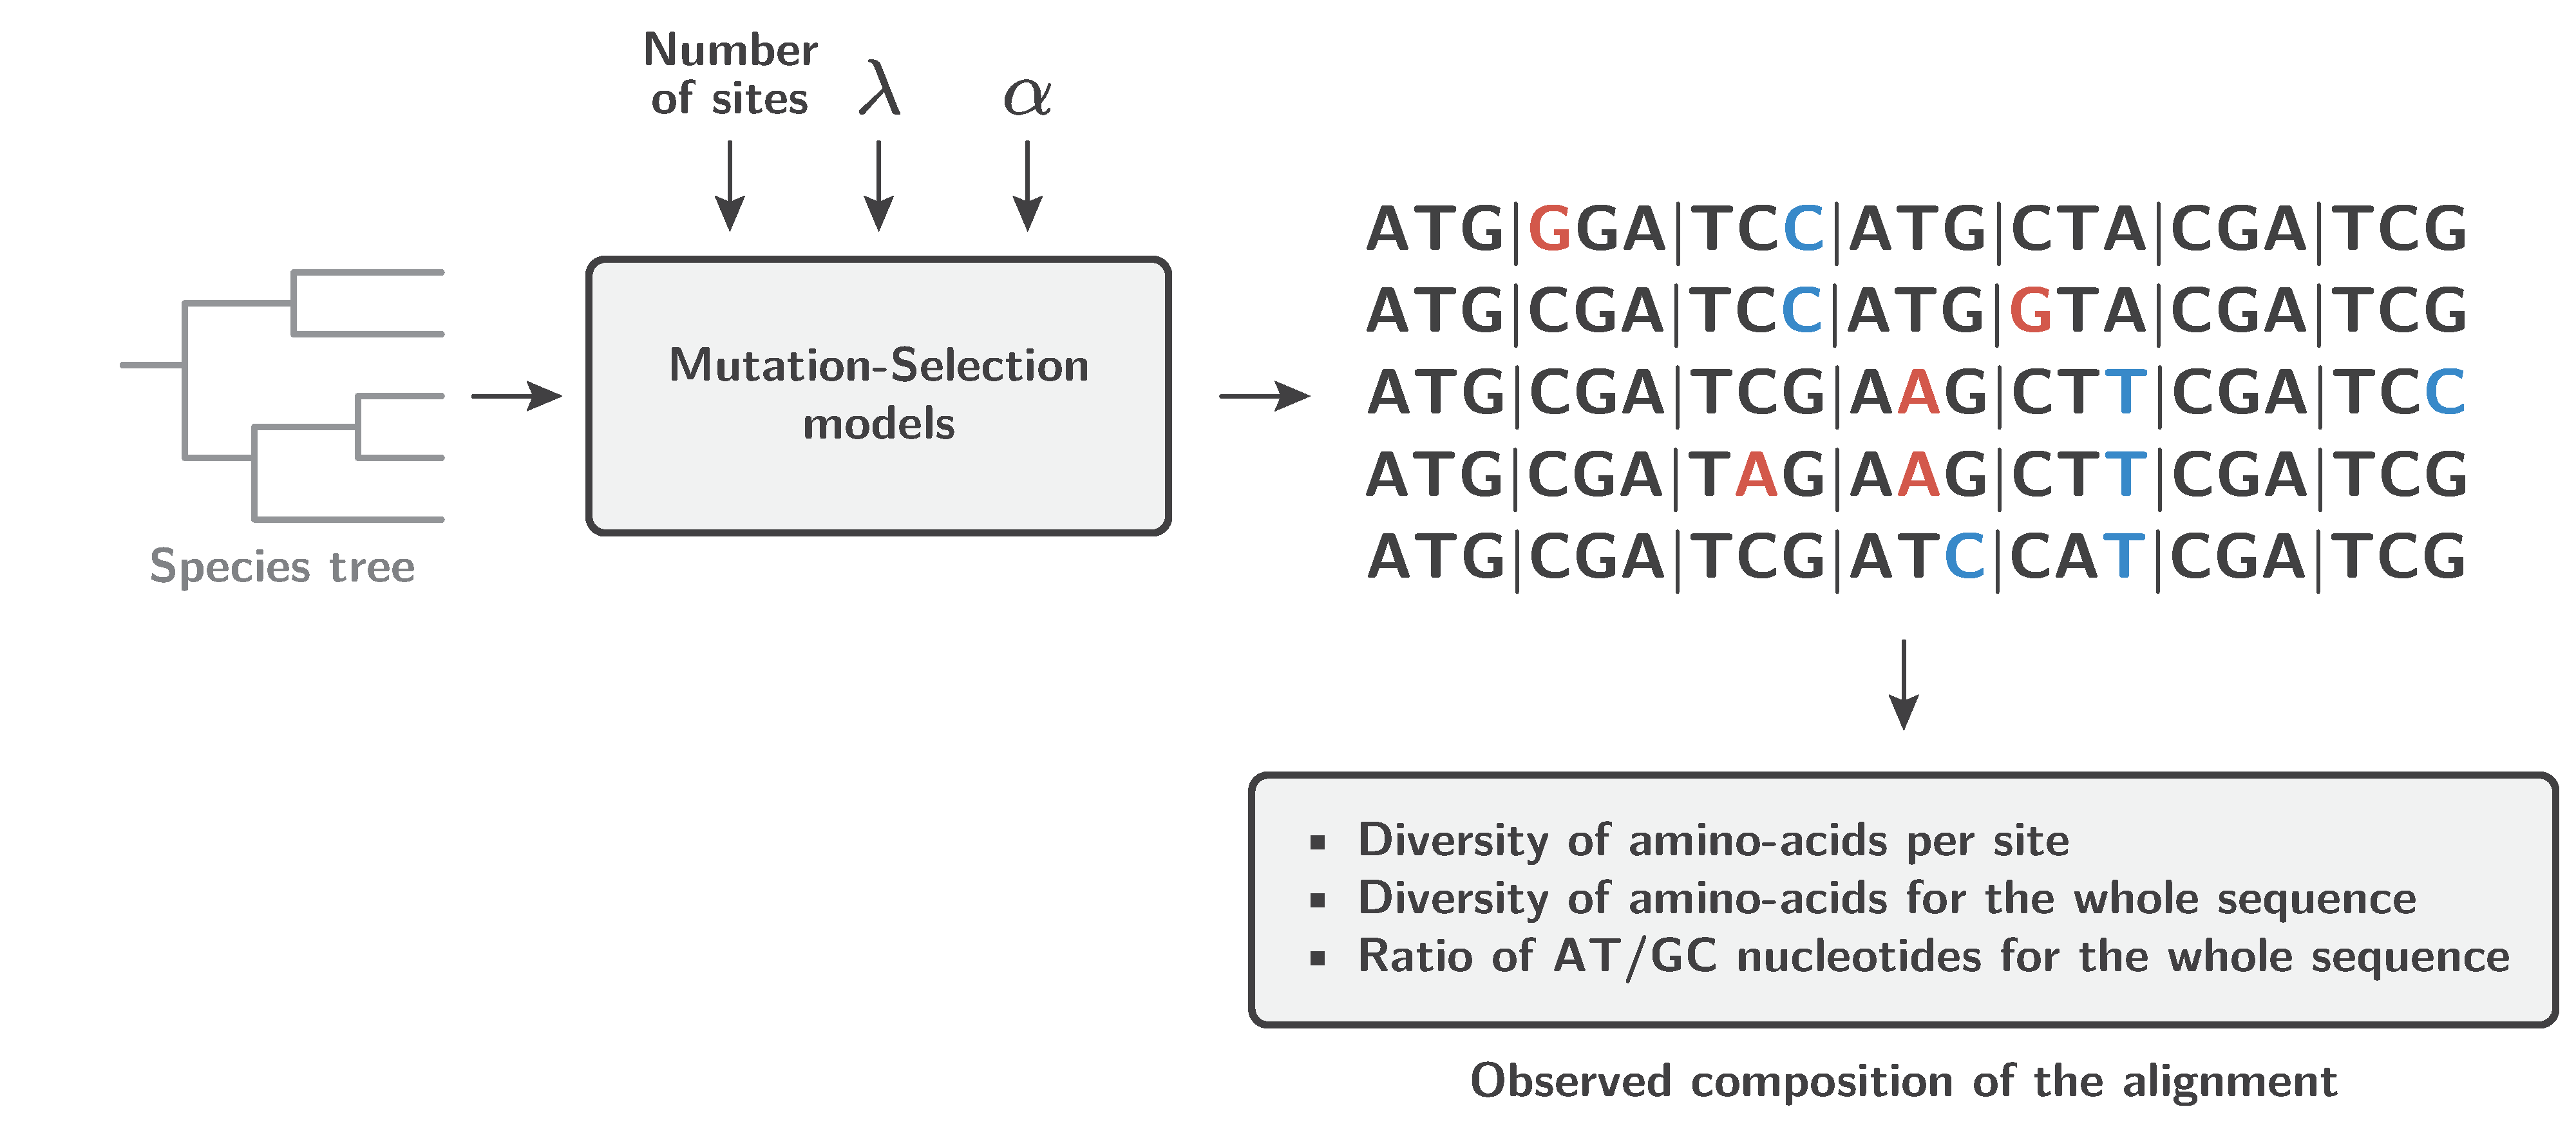
\includegraphics[width=\textwidth] {figures/mut-bias-simulations}
	\end{center}
	\caption[Simulations and analysis]{Simulations and analysis. We can observe composition of the alignment as function of the mutation and selection parameters.}
\end{figure}

\subsection{AT/GC as a function of the mutation-selection model}
The codon substitution process, at site $k$, which takes into account mutation and selection, is a function of $\lambda$ and $F^{(k)}$. Moreover this process has stationary distribution $\pi^{(k)}$. From this equilibrium frequency of codons, we define $\mathrm{AT_{obs}}^{(k)}(\lambda, F^{(k)})$ as the observed stationary distribution of weak nucleotides at site $k$:
\begin{align}
\mathrm{AT_{obs}}^{(k)}(\lambda, F^{(k)})
& =\frac{1}{3} \sum_{x \in \SetCodon} \Pi_x^{(k)} w_x , \ \textrm{by definition},\\
& =\frac{A^{(k)}}{3} \sum_{x \in \SetCodon} \lambda^{w_x} \e^{F_X^{(k)}} w_x , \ \textrm{from eq.} \ \ref{codonStationarity}.
\label{atPctSite}
\end{align}
As noted in \ref{sec:mutBias}, the mutational process leads to $(\pi_A+\pi_T)/(\pi_C+\pi_G) = \lambda$. Similarly, we denote the observed ratio of weak over strong nucleotide frequency, at site $k$, as $\lambda_{\mathrm{obs}}^{(k)} (\lambda, F^{(k)})$:
\begin{align}
\lambda_{\mathrm{obs}}^{(k)} (\lambda, F^{(k)})
& =\dfrac{\mathrm{AT_{obs}}^{(k)}(\lambda, F^{(k)})}{1 - \mathrm{AT_{obs}}^{(k)}(\lambda, F^{(k)}) }, \ \textrm{by definition},\\
& =\dfrac{ \sum_{x \in \SetCodon} \lambda^{w_x} \e^{F_X^{(k)}} w_x}{\sum_{x \in \SetCodon} \lambda^{w_x} \e^{F_X^{(k)}} (3 - w_x )}, \ \textrm{from eq.} \ \ref{atPctSite}.
\end{align}
At the sequence level, $\mathrm{AT_{obs}}(\lambda, \bm{F})$ is the observed stationary distribution of weak nucleotides:
\begin{align}
\mathrm{AT_{obs}}(\lambda, \bm{F})
& =\frac{1}{n}\sum_{k=1}^{n} \mathrm{AT_{obs}}^{(k)}(\lambda, F^{(k)}), \ \textrm{by definition}, \\
& =\frac{1}{3n}\sum_{k=1}^{n} \sum_{x \in \SetCodon} A^{(k)} \lambda^{w_x} \e^{F_X^{(k)}} w_x , \ \textrm{from eq.} \ \ref{atPctSite}.
\label{atPctSeq}
\end{align}
Similarly, we denote the observed ratio of weak over strong nucleotide frequency, for the whole sequence, as $\lambda_{\mathrm{obs}} (\lambda, \bm{F})$
\begin{align}
\lambda_{\mathrm{obs}} (\lambda, \bm{F})
& = \frac{\mathrm{AT_{obs}}(\lambda, \bm{F})}{ 1 - \mathrm{AT_{obs}}(\lambda, \bm{F}) }, \ \textrm{by definition},\\
& =\dfrac{ \sum_{k=1}^{n}  A^{(k)} \sum_{x \in \SetCodon} \lambda^{w_x} \e^{F_X^{(k)}} w_x}{ \sum_{k=1}^{n} A^{(k)} \sum_{x \in \SetCodon} \lambda^{w_x} \e^{F_X^{(k)}} (3 - w_x )}, \ \textrm{from eq.} \ \ref{atPctSeq}.
\end{align}
We then consider amino-acids propensities $S$ (exponential of fitnesses) as a multivariate continuous random variable. More specifically $S$ follow a Dirichlet distribution with concentration parameter $\alpha$.
\begin{equation}
S \sim \mathrm{Dirichlet}(\alpha, 20).
\end{equation}
Under a Dirichlet distribution of amino-acids propensities, the expected observed stationary distribution of weak nucleotides $\operatorname{E} [\mathrm{AT_{obs}}(\lambda, S)]$ is:
\begin{align}
\operatorname{E} [\mathrm{AT_{obs}}(\lambda, S)]
& =\int_{C(s)} \mathrm{AT_{obs}}(\lambda, s) p(s) \der s, \ \textrm{by defintion}, \\
& =\frac{1}{3} \int_{C(s)} A(\lambda, s) \sum_{x \in \SetCodon} 
\lambda^{w_x} s_X w_x p(s) \der s, \ \textrm{from eq.} \ \ref{atPctSite}, \\
& =\frac{1}{3} \int_{ C(s)} A(\lambda, s) \sum_{x \in \SetCodon}  \lambda^{w_x} s_X w_x {\frac {\Gamma (20 \alpha)}{\Gamma (\alpha )^{20}}} \prod_{Y \in \SetAa} s_Y^{\alpha-1} \der s, \\
& ={\frac {\Gamma (20 \alpha)}{3\Gamma (\alpha )^{20}}} \sum_{x \in \SetCodon} \lambda^{w_x} w_x  \int_{ C(s)} A(\lambda, s) s_X \prod_{Y \in \SetAa} s_Y^{\alpha-1} \der s, \\
& ={\frac {\Gamma (20 \alpha)}{3\Gamma (\alpha )^{20}}} \sum_{x \in \SetCodon} \lambda^{w_x} w_x \int_{ C(s)} s_X \dfrac{\prod_{Y \in \SetAa} s_Y^{\alpha-1}}{\sum_{y \in \SetCodon} \lambda^{w_y} s_Y} \der s, \\
& ={\frac {\Gamma (20 \alpha)}{3\Gamma (\alpha )^{20}}} \sum_{x \in \SetCodon} \lambda^{w_x} w_x \Phi_X(\lambda, \alpha),\\
&  \textrm{where} \  \Phi_X(\lambda, \alpha) = \int_{ C(s)} s_X \dfrac{\prod_{Y \in \SetAa} s_Y^{\alpha}}{\sum_{y \in \SetCodon} \lambda^{w_y} s_Y}\der s.
\label{atPctSeqExpected}
\end{align}
Similarly, the observed ratio of weak over strong nucleotide frequency, for the whole sequence, as $\operatorname{E} [\lambda_{\mathrm{obs}}(\lambda, S)]$: 
\begin{align}
\operatorname{E} [\lambda_{\mathrm{obs}}(\lambda, S)]
& =\frac{\operatorname{E} [\mathrm{AT_{obs}}(\lambda, S)]}{ 1 - \operatorname{E} [\mathrm{AT_{obs}}(\lambda, S)] }, \ \textrm{by definition},\\
& =\frac{\sum_{x \in \SetCodon} \lambda^{w_x} w_x \Phi_X(\lambda, \alpha)}{\sum_{x \in \SetCodon} \lambda^{w_x} (3 - w_x) \Phi_X(\lambda, \alpha)}, \ \textrm{from eq.} \ \ref{atPctSeqExpected}.
\label{atgcPctSeqExpected}
\end{align}
For a large sequence ($ n \gg 1 $), $\lambda_{\mathrm{obs}} (\lambda, \bm{F})$ converges to $\operatorname{E} [\lambda_{\mathrm{obs}}(\lambda, S)]$:
\begin{align}
\lambda_{\mathrm{obs}} (\lambda, \bm{F})
& \simeq \operatorname{E} [\lambda_{\mathrm{obs}}(\lambda, S)],\\
& =\frac{\sum_{x \in \SetCodon} \lambda^{w_x} w_x \Phi_X(\lambda, \alpha)}{\sum_{x \in \SetCodon} \lambda^{w_x} (3 - w_x) \Phi_X(\lambda, \alpha)}, \ \textrm{from eq.} \ \ref{atgcPctSeqExpected}.
\end{align}

\begin{figure}[thbp]
	\begin{center}
		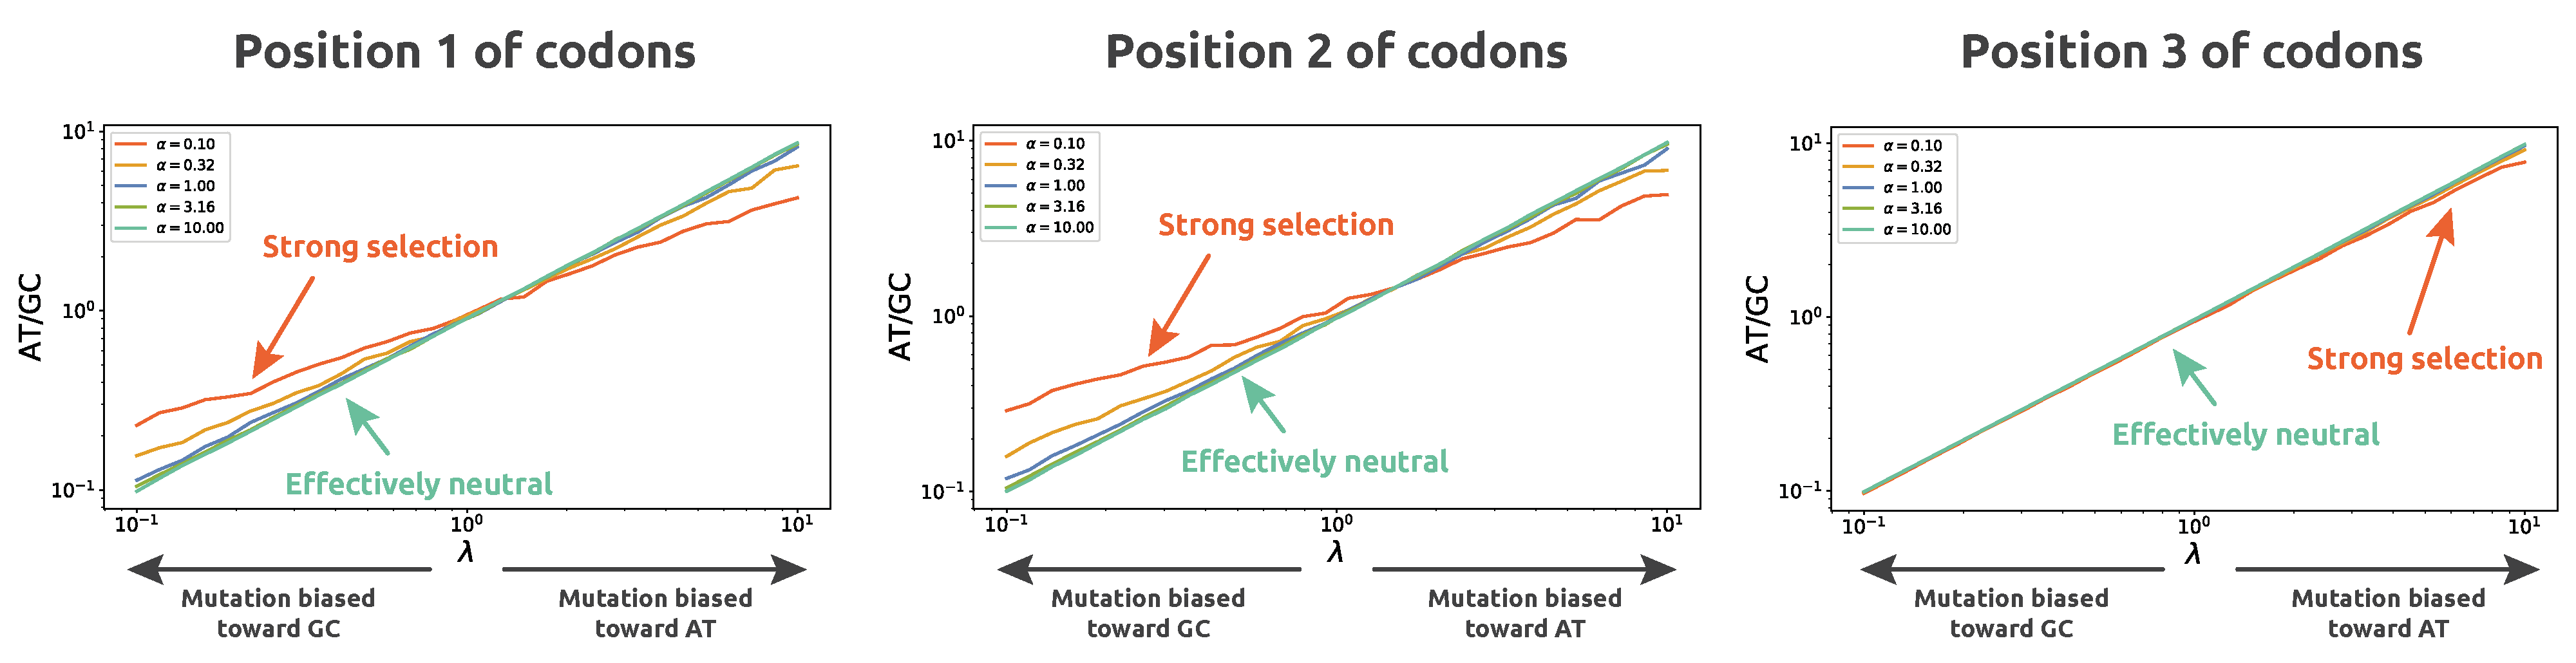
\includegraphics[width=\textwidth] {figures/mut-bias-AT-GC-obs}
	\end{center}
	\caption[AT/GC composition of the alignment]{AT/GC composition of the alignment. Observed AT/GC at the third codon position matches the mutational bias. Selection is balancing the mutational bias.}
\end{figure}

\subsection{Diversity of codons as a function of the mutation-selection model}

The evolutionary variability of an amino acid site in a protein family is an important indicator of the selective constraints that the site experiences. This variability is usually quantified either through the sequence entropy \citep{Goldstein2017}

Our analysis highlights how important it is to distinguish between amino acid frequencies averaged over a large class of sites with similar property (such as RSA) and amino acid frequencies at individual sites. In both cases, frequencies are Boltzmann distributed, and thus it is easy to mistake one for the other. However, the properties of these two distributions are very different. For example, in yeast, at sites with RSA close to 0.2 nearly all amino acids occur at comparable frequencies. Yet at any given site, only a small number ofamino acids are actually permissible. Evolutionary rate, which measures the rate at which mutations at individual sites arise and go to fixation, is governed by the amino acid distribution of individual sites, not the average distribution over a broad class of sites. \citep{Ramsey2011}

The codon substitution process, at site $k$, which takes into account mutation and selection, is a function of $\lambda$ and $F^{(k)}$. Moreover this process has stationary distribution $\pi^{(k)}$. From this equilibrium frequency of codons, we can compute the effective number of codon, mathematically this correspond to the diversity of the distribution $D^{(k)}$, at site $k$:
\begin{align}
D^{(k)}(\lambda, F^{(k)})
& =\e^{ - \sum_{x \in \SetCodon}  \Pi_x^{(k)} \ln ( \Pi_x^{(k)} )}, \ \textrm{by definition},\\
& =\e^{ - \sum_{x \in \SetCodon}  \Pi_x^{(k)} \ln \left( A^{(k)} \lambda^{w_x} \e^{F_X^{(k)}} \right)}, \ \textrm{from eq.} \ \ref{codonStationarity},\\
& =\e^{ - \sum_{x \in \SetCodon}  \Pi_x^{(k)} \left[ \ln ( A^{(k)} )+ \ln( \lambda^{w_x} ) + \ln (\e^{F_X^{(k)}}) \right] }\\
& =\e^{ - \ln ( A^{(k)} ) \sum_{x \in \SetCodon}  \Pi_x^{(k)} } \e^{ -  \ln (\lambda) \sum_{x \in \SetCodon}  \Pi_x^{(k)} w_x }\e^{ - \sum_{x \in \SetCodon}  \Pi_x^{(k)} F_X^{(k)}  } \\
& =\frac{1}{A^{(k)}} \e^{ -  \ln (\lambda) \sum_{x \in \SetCodon}  \Pi_x^{(k)} w_x }\e^{ - \sum_{x \in \SetCodon}  \Pi_x^{(k)} F_X^{(k)}  }
\label{entropy}
\end{align}

\begin{figure}[thbp]
	\begin{center}
		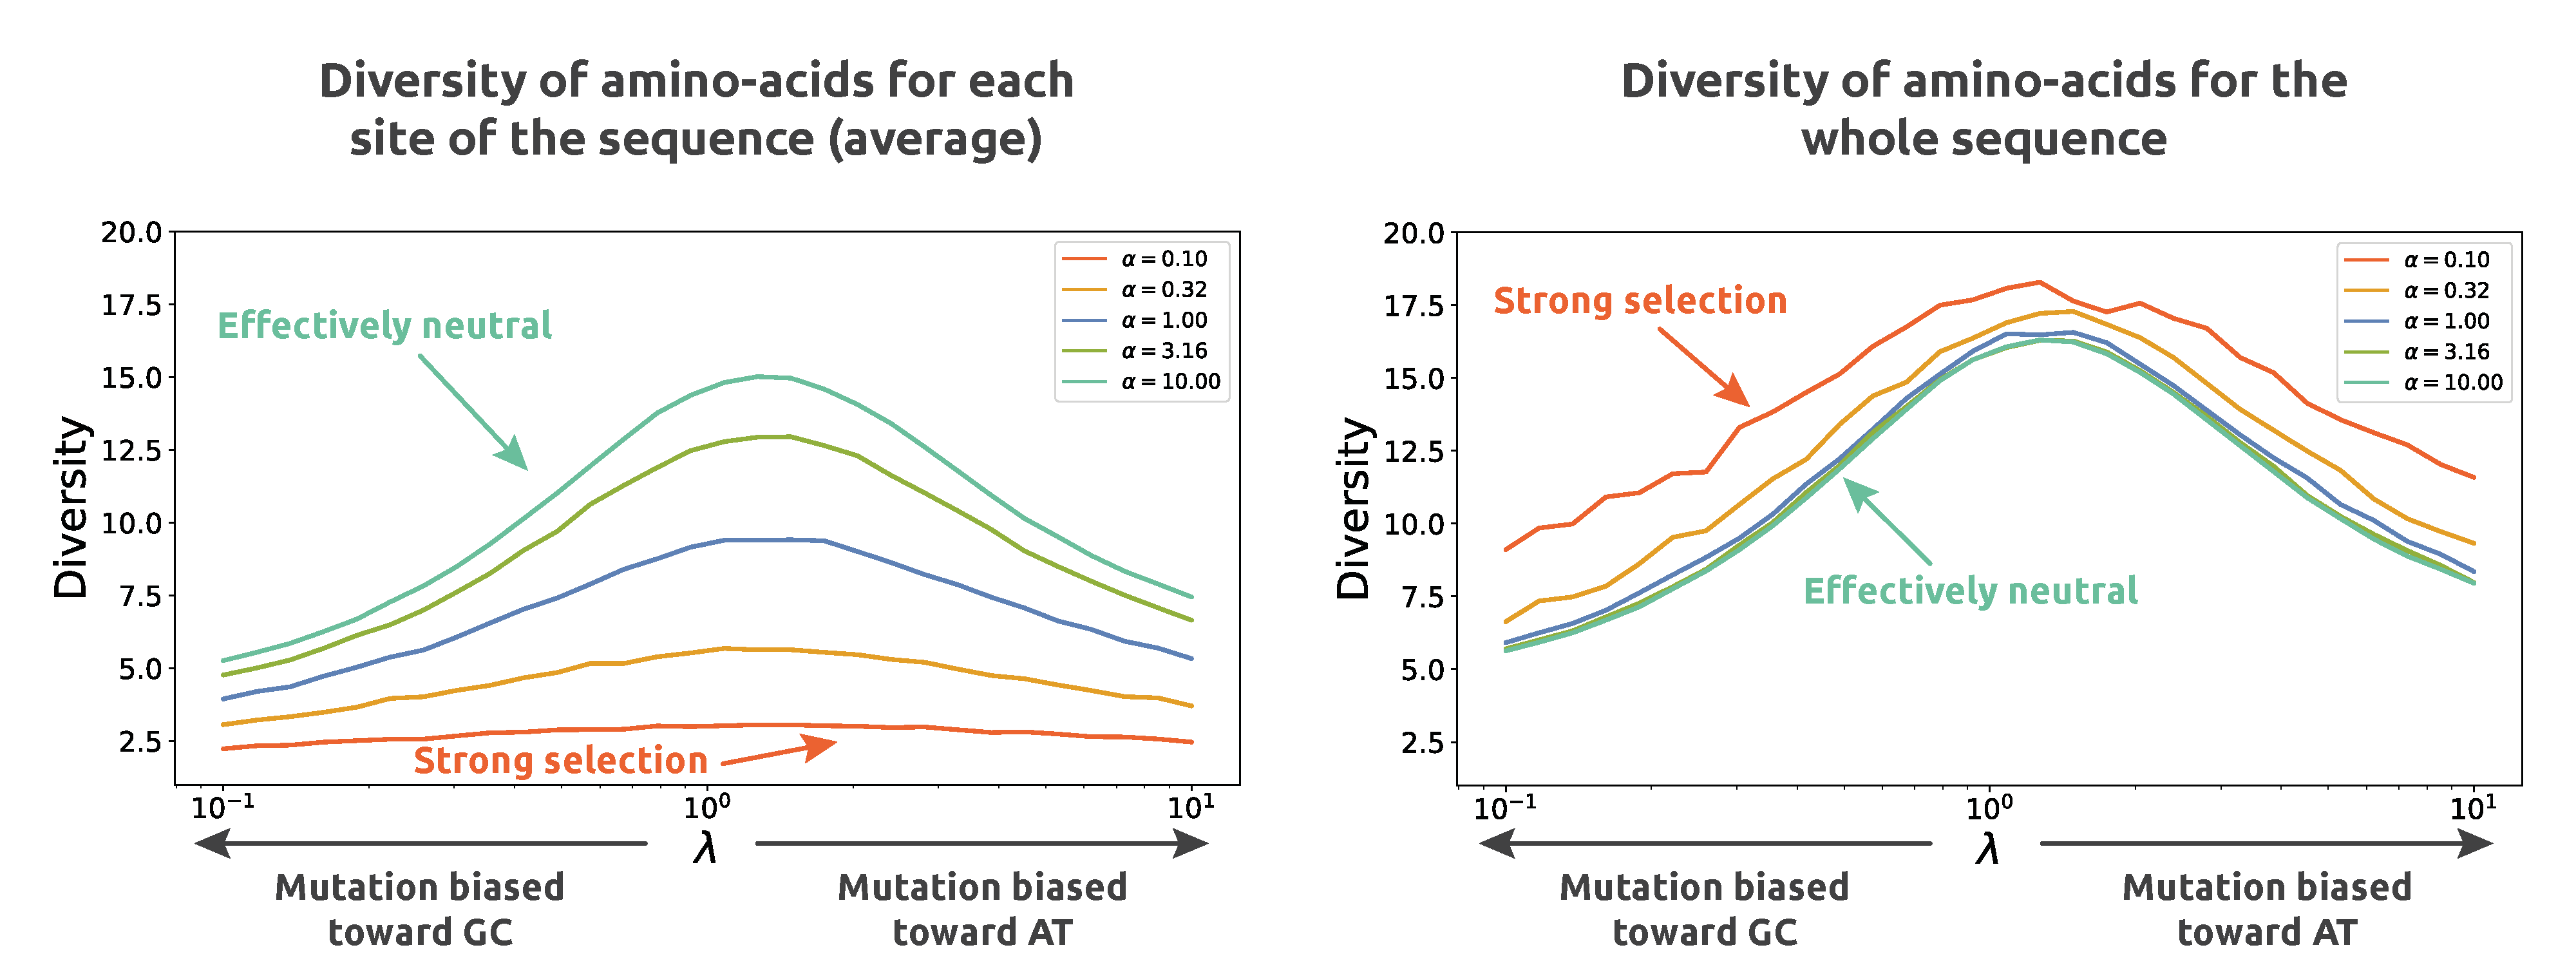
\includegraphics[width=\textwidth] {figures/mut-bias-diversity-aa}
	\end{center}
	\caption[Diversity of amino-acids]{Diversity of amino-acids. Sequence-diversity is higher than site-diversity. Diversity decreases with mutational bias.	Site-diversity decreases with selection. Sequence-diversity increase with selection.}
\end{figure}

\subsection{dN/dS as a function of the mutation-selection model}
The substitution rate (e.g., Grishin, Wolf \& Koonin, 2000). These two measures of evolutionary variability are considered to be essentially equivalent \citep{Halpern1998}, though they are differently influenced by the mutational process \citep{Santos2018}

The codon substitution process, at site $k$, which takes into account mutation and selection, is a function of $\lambda$ and $F^{(k)}$. Moreover this process has stationary distribution $\pi^{(k)}$. From this equilibrium frequency of codons, we define $L_{\NonSyn}^{(k)}(\lambda, F^{(k)})$ as the non-synonymous substitution flow, at site $k$:
\begin{align}
L_{\NonSyn}^{(k)}(\lambda, F^{(k)})
& =  \sum_{x \in \SetCodon} \sum_{y \in \NxNonSyn} \Pi_x^{(k)} Q_{x, y}^{(k)}, \ \textrm{by definition},\\
& =\sum_{x \in \SetCodon} \sum_{y \in \NxNonSyn} A^{(k)} \lambda^{w_x} \e^{F_X^{(k)}} U_{x, y} \dfrac{F_Y^{(k)} - F_X^{(k)}}{1 - \e^{F_X^{(k)} - F_Y^{(k)}}}, \ \textrm{from eq.}\ \ref{codonSubRates} \ \text{and} \ \ref{codonStationarity},\\
& =A^{(k)} \sum_{x \in \SetCodon} \lambda^{w_x} \sum_{y \in \NxNonSyn}  U_{x, y} \dfrac{F_Y^{(k)} - F_X^{(k)}}{\e^{-F_X^{(k)}} - \e^{ - F_Y^{(k)}}}.
\label{subFlowNonSyn}
\end{align}
Moreover, we define $K_{\NonSyn}^{(k)}(\lambda, F^{(k)})$ as the non-synonymous mutation flow, at site $k$:
\begin{align}
K_{\NonSyn}^{(k)}(\lambda, F^{(k)})
& =  \sum_{x \in \SetCodon} \sum_{y \in \NxNonSyn} \Pi_x^{(k)} U_{x, y}, \ \textrm{by definition},\\
& = A^{(k)}  \sum_{x \in \SetCodon} \lambda^{w_x} \sum_{y \in \NxNonSyn} \e^{F_X^{(k)}} U_{x, y}, \ \textrm{from eq.}\ \ref{codonSubRates} \ \text{and} \ \ref{codonStationarity}.
\label{mutFlowNonSyn}
\end{align}
We also define the mutation and substitution synonymous as $K_{\Syn}^{(k)}(\lambda, F^{(k)})$ and $L_{\Syn}^{(k)}(\lambda, F^{(k)})$ respectively:
\begin{align}
L_{\Syn}^{(k)}(\lambda, F^{(k)})
& =  \sum_{x \in \SetCodon} \sum_{y \in \NxSyn} \Pi_x^{(k)} Q_{x, y}^{(k)}, \ \textrm{by definition},\\
& =\sum_{x \in \SetCodon} \sum_{y \in \NxSyn} A^{(k)} \lambda^{w_x} \e^{F_X^{(k)}} U_{x, y}, \ \textrm{from eq.}\ \ref{codonSubRates} \ \text{and} \ \ref{codonStationarity}, \\
& =K_{\Syn}^{(k)}(\lambda, F^{(k)})
\label{subFlowSyn}
\end{align}
Following Spielman and Wilke \citep{Spielman2015}, the rate of non-synonymous to synonymous substitution is thus :
\begin{align}
\omega^{(k)}(\lambda, F^{(k)})
& =\dfrac{L_{\NonSyn}^{(k)}(\lambda, F^{(k)})}{K_{\NonSyn}^{(k)}(\lambda, F^{(k)})}  \left( \dfrac{L_{\Syn}^{(k)}(\lambda, F^{(k)})}{K_{\Syn}^{(k)}(\lambda, F^{(k)})}  \right)^{-1}, \\
& =\dfrac{L_{\NonSyn}^{(k)}(\lambda, F^{(k)})}{K_{\NonSyn}^{(k)}(\lambda, F^{(k)})}, \ \textrm{from eq.}\ \ref{subFlowSyn} \\
& =\dfrac{ \sum_{x \in \SetCodon} \lambda^{w_x} \sum_{y \in \NxNonSyn}  U_{x, y} \dfrac{F_Y^{(k)} - F_X^{(k)}}{\e^{ - F_Y^{(k)}} -  \e^{- F_X^{(k)}} } }{ \sum_{x \in \SetCodon}  \lambda^{w_x} \sum_{y \in \NxNonSyn} U_{x, y} \e^{F_X^{(k)}} }, \ \textrm{from eq.}\ \ref{subFlowNonSyn} \ \text{and} \ \ref{mutFlowNonSyn}.
\label{omegaSite}
\end{align}
The non-synonymous over synonymous rate for the whole sequence is then given by:
\begin{align}
\omega(\lambda, \bm{F})
& =\dfrac{\sum_{k=1}^{n} L_{\NonSyn}^{(k)}(\lambda, F^{(k)})}{\sum_{k=1}^{n}K_{\NonSyn}^{(k)}(\lambda, F^{(k)})}  \left( \dfrac{\sum_{k=1}^{n}L_{\Syn}^{(k)}(\lambda, F^{(k)})}{\sum_{k=1}^{n}K_{\Syn}^{(k)}(\lambda, F^{(k)})}  \right)^{-1}, \\
& =\dfrac{\sum_{k=1}^{n} L_{\NonSyn}^{(k)}(\lambda, F^{(k)})}{\sum_{k=1}^{n}K_{\NonSyn}^{(k)}(\lambda, F^{(k)})}, \ \textrm{from eq.}\ \ref{subFlowSyn} \\
& =\dfrac{ \sum_{k=1}^{n} \sum_{x \in \SetCodon} \lambda^{w_x} \sum_{y \in \NxNonSyn}  U_{x, y} \dfrac{F_Y^{(k)} - F_X^{(k)}}{\e^{ - F_Y^{(k)}} -  \e^{- F_X^{(k)}} } }{ \sum_{k=1}^{n} \sum_{x \in \SetCodon}  \lambda^{w_x}  \sum_{y \in \NxNonSyn} U_{x, y} \e^{F_X^{(k)}}}, \ \textrm{from eq.}\ \ref{subFlowNonSyn} \ \text{and} \ \ref{mutFlowNonSyn}. \\
& =\dfrac{ \sum_{x \in \SetCodon} \lambda^{w_x} \sum_{y \in \NxNonSyn}  U_{x, y}  \sum_{k=1}^{n} \dfrac{F_Y^{(k)} - F_X^{(k)}}{\e^{ - F_Y^{(k)}} -  \e^{- F_X^{(k)}} } }{  \sum_{x \in \SetCodon}  \lambda^{w_x}  \sum_{y \in \NxNonSyn} U_{x, y}  \sum_{k=1}^{n} \e^{F_X^{(k)}}}.
\label{omegaSeq}
\end{align}
We then consider amino-acids propensities $S$ (exponential of fitnesses) as a multivariate continuous random variable. More specifically $S$ follow a Dirichlet distribution with concentration parameter $\alpha$.
\begin{equation}
S \sim \mathrm{Dirichlet}(\alpha, 20).
\end{equation}
Under a Dirichlet distribution of amino-acids propensities, the expected non-synonymous substitution flow $\operatorname{E} [L_{\NonSyn}(\lambda, S)]$ :
\begin{align}
\operatorname{E} [L_{\NonSyn}(\lambda, S)]
& =\int_{C(s)} L_{\NonSyn}(\lambda, s) p(s) \der s, \ \textrm{by defintion}, \\
& =\int_{C(s)} A(\lambda, s) \sum_{x \in \SetCodon} \lambda^{w_x} \sum_{y \in \NxNonSyn} U_{x, y} s_X s_Y\dfrac{\ln(s_Y)-\ln(s_X)}{s_Y - s_Y} p(s) \der s , \ \textrm{from eq.}\ \ref{subFlowNonSyn}, \\
& =\int_{C(s)} A(\lambda, s) \sum_{x \in \SetCodon} \lambda^{w_x} \sum_{y \in \NxNonSyn} U_{x, y} s_X s_Y\dfrac{\ln(s_Y)-\ln(s_X)}{s_Y - s_Y} {\frac {\Gamma (20 \alpha)}{\Gamma (\alpha )^{20}}} \prod_{X \in \SetAa} s_X^{\alpha-1} \der s,\\
& ={\frac {\Gamma (20 \alpha)}{\Gamma (\alpha )^{20}}} \sum_{x \in \SetCodon} \lambda^{w_x} \sum_{y \in \NxNonSyn} U_{x, y} \int_{C(s)} s_Y\dfrac{\ln(s_Y)-\ln(s_X)}{s_Y - s_Y} \dfrac{\prod_{X \in \SetAa} s_X^{\alpha}}{\sum_{y \in \SetCodon} \lambda^{w_y} s_Y} \der s.\\
& ={\frac {\Gamma (20 \alpha)}{\Gamma (\alpha )^{20}}} \sum_{x \in \SetCodon} \lambda^{w_x} \sum_{y \in \NxNonSyn} U_{x, y} \Psi(\lambda, \alpha), \\
& \textrm{where} \ \Psi(\lambda, \alpha) = \int_{C(s)} s_Y\dfrac{\ln(s_Y)-\ln(s_X)}{s_Y - s_Y} \dfrac{\prod_{X \in \SetAa} s_X^{\alpha}}{\sum_{y \in \SetCodon} \lambda^{w_y} s_Y} \der s.
\end{align}
Moreover, the expected non-synonymous mutation flow $\operatorname{E} [K_{\NonSyn}(\lambda, S)]$ is:
\begin{align}
\operatorname{E} [K_{\NonSyn}(\lambda, S)]
& =  \int_{C(s)} K_{\NonSyn}(\lambda, s) p(s) \der s, \ \textrm{by defintion}, \\
& =\int_{C(s)} A(\lambda, s) \sum_{x \in \SetCodon} \lambda^{w_x} \sum_{y \in \NxNonSyn} s_X U_{x, y} p(s) \der s , \ \textrm{from eq.}\ \ref{mutFlowNonSyn}, \\
& =\int_{C(s)} A(\lambda, s) \sum_{x \in \SetCodon} \lambda^{w_x} \sum_{y \in \NxNonSyn} s_X U_{x, y}{\frac {\Gamma (20 \alpha)}{\Gamma (\alpha )^{20}}} \prod_{X \in \SetAa} s_X^{\alpha-1} \der s,\\
& =\frac{\Gamma (20 \alpha)}{\Gamma (\alpha )^{20}} \sum_{x \in \SetCodon} \lambda^{w_x} \sum_{y \in \NxNonSyn} U_{x, y} \int_{C(s)} \dfrac{\prod_{X \in \SetAa} s_X^{\alpha}}{\sum_{y \in \SetCodon} \lambda^{w_y} s_Y}\der s,\\
& =\frac{\Gamma (20 \alpha)}{\Gamma (\alpha )^{20}} \sum_{x \in \SetCodon} \lambda^{w_x} \sum_{y \in \NxNonSyn} U_{x, y} \Phi(\lambda, \alpha).\\
\end{align}
The expected non-synonymous over synonymous rate, $\operatorname{E} [\omega(\lambda, S)]$ , is then given by:
\begin{align}
\operatorname{E} [\omega(\lambda, S)]
& =  \dfrac{\operatorname{E} [L_{\NonSyn}(\lambda, S)]}{\operatorname{E} [K_{\NonSyn}(\lambda, S)]} \\
& =\dfrac{\sum_{x \in \SetCodon} \lambda^{w_x} \sum_{y \in \NxNonSyn} U_{x, y} \Psi(\lambda, \alpha)}{\sum_{x \in \SetCodon} \lambda^{w_x} \sum_{y \in \NxNonSyn} U_{x, y} \Phi(\lambda, \alpha)}.
\label{omegaExpected}
\end{align}
For a large sequence ($ n \gg 1 $), $\omega (\lambda, \bm{F})$ converges to $\operatorname{E} [\omega(\lambda, S)]$:
\begin{align}
\omega (\lambda, \bm{F})
& \simeq \operatorname{E} [\omega(\lambda, S)],\\
& =\dfrac{\sum_{x \in \SetCodon} \lambda^{w_x} \sum_{y \in \NxNonSyn} U_{x, y} \Psi(\lambda, \alpha)}{\sum_{x \in \SetCodon} \lambda^{w_x} \sum_{y \in \NxNonSyn} U_{x, y} \Phi(\lambda, \alpha)}, \ \textrm{from eq.} \ \ref{omegaExpected}.
\end{align}

\begin{figure}[thbp]
	\begin{center}
		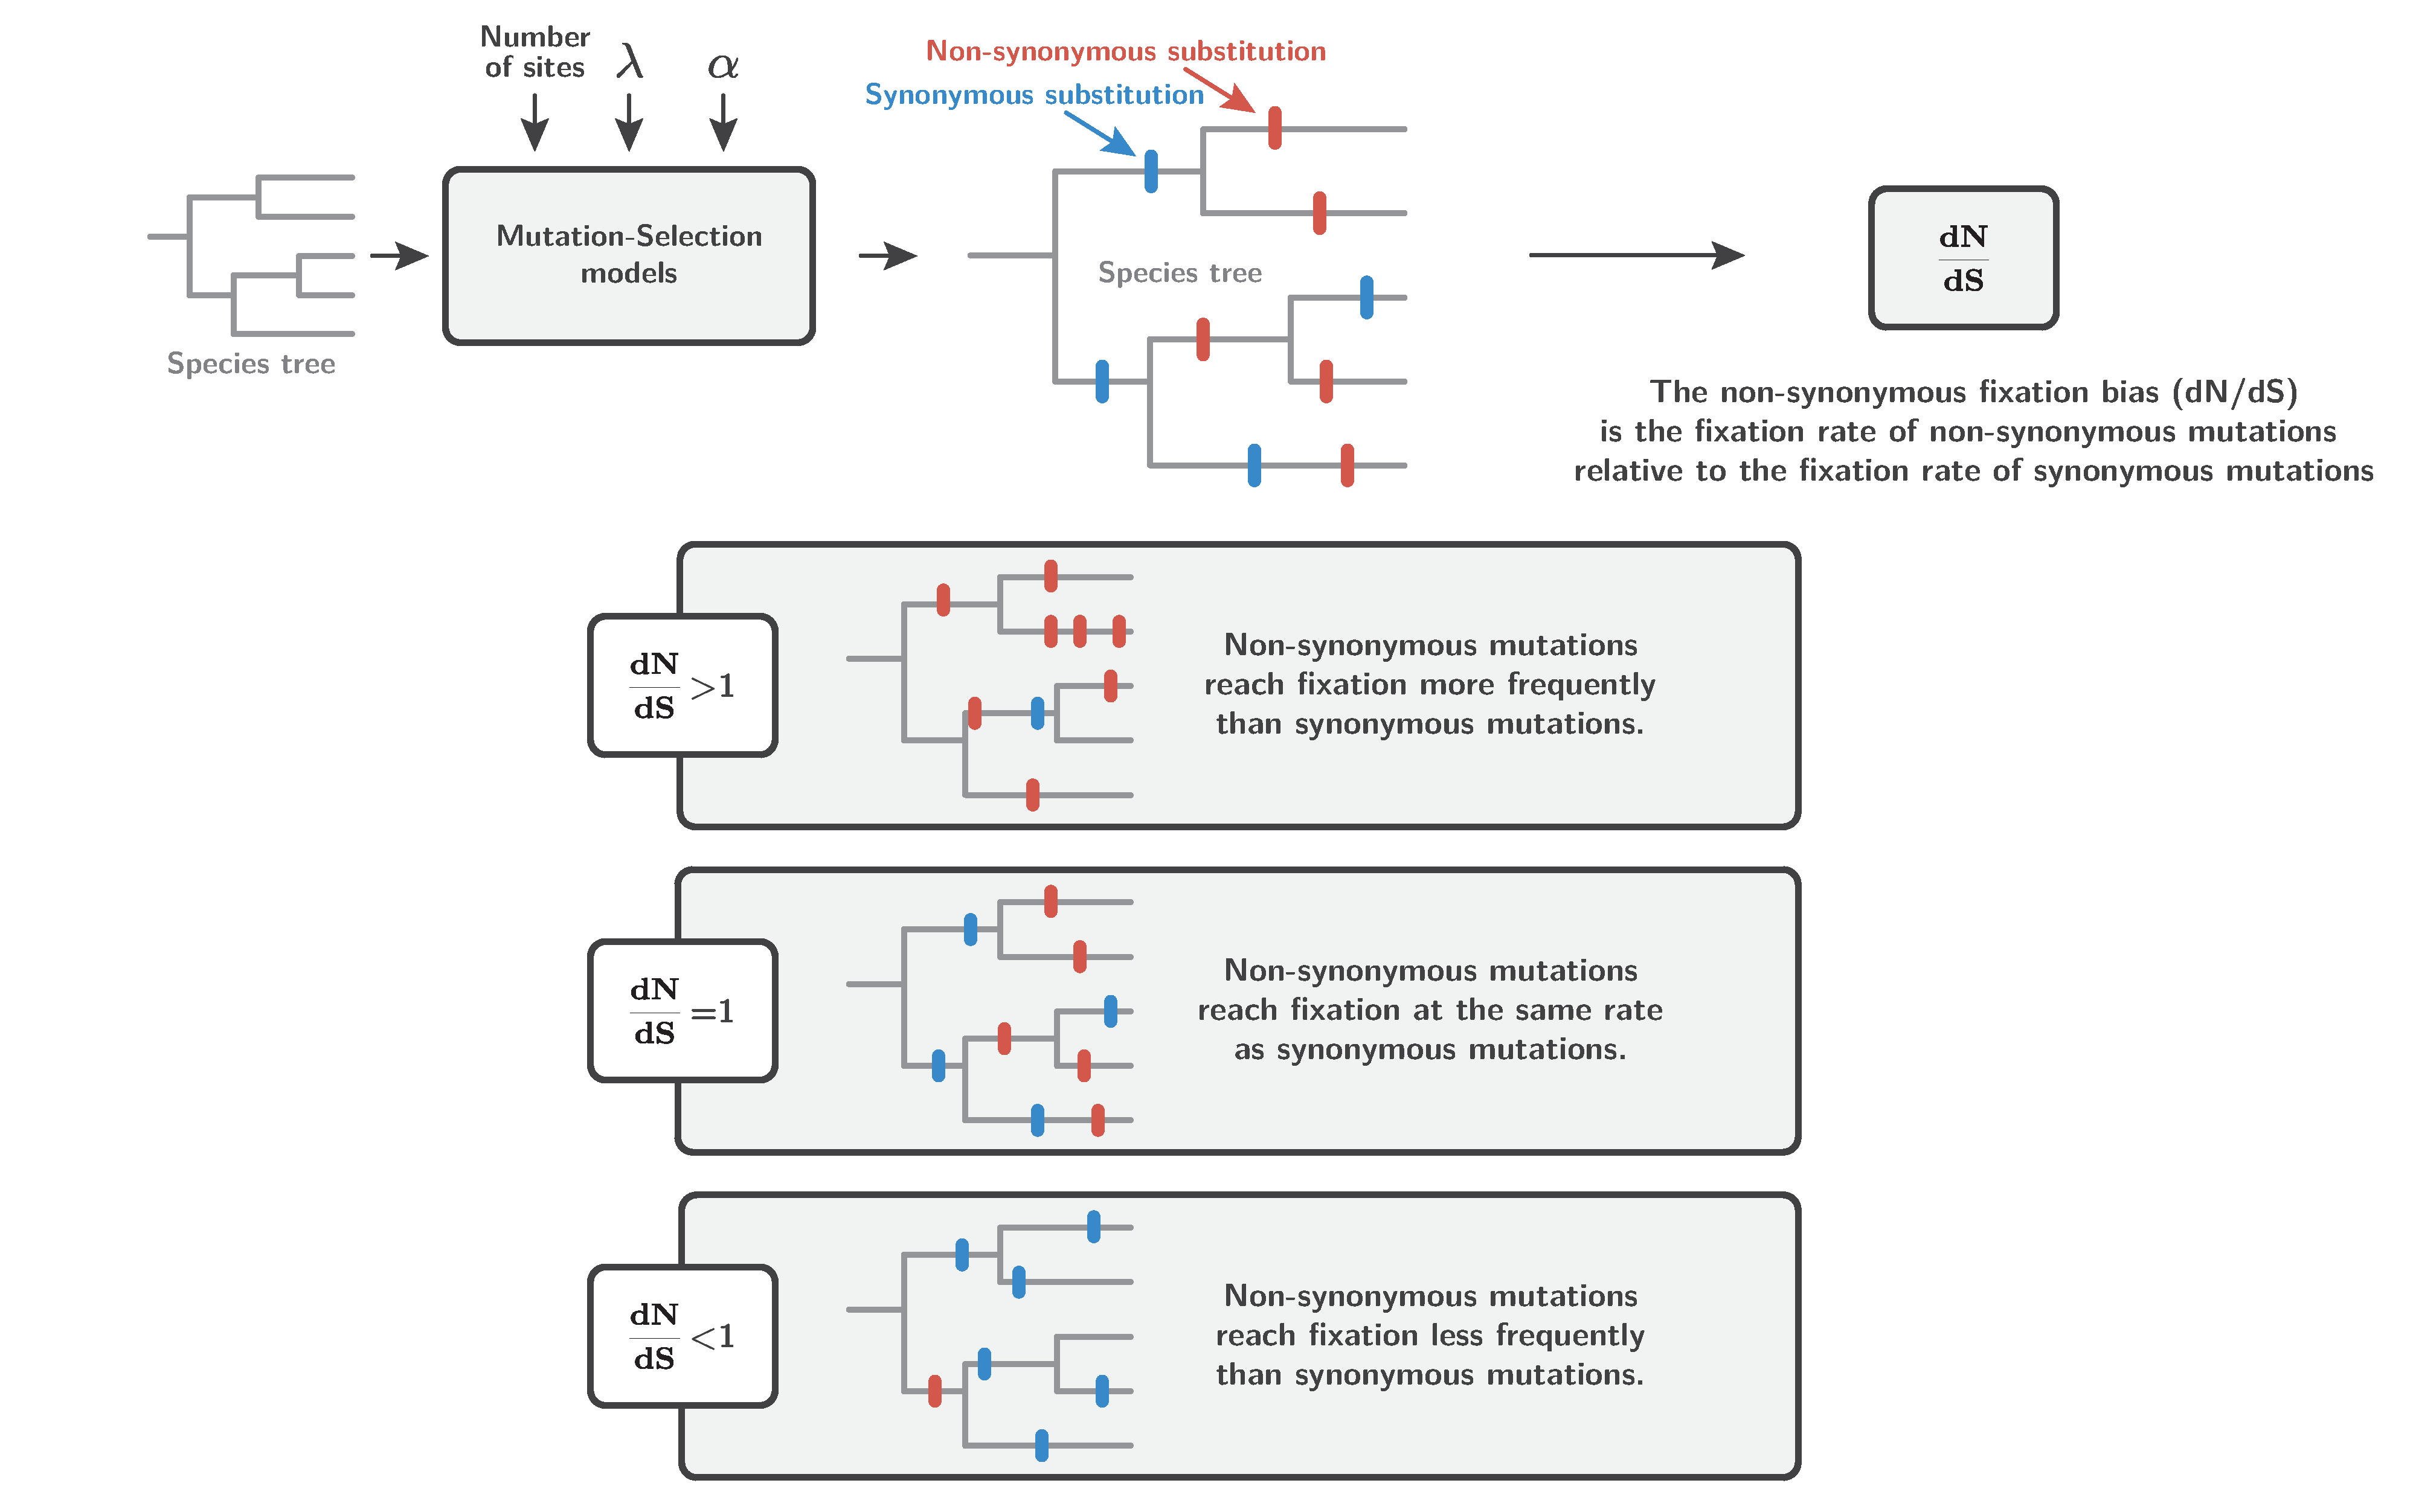
\includegraphics[width=\textwidth] {figures/mut-bias-definitions}
	\end{center}
	\caption[Definition of $\omega$]{Definition of $\omega$.}
\end{figure}

\begin{figure}[thbp]
	\begin{center}
		\includegraphics[width=\textwidth] {figures/mut-bias-omega}
	\end{center}
	\caption[$\omega$ as a function of the parameters]{$\omega$ as a function of the parameters. Non-synonymous fixation bias is always lower than. Non-synonymous fixation bias decrease with the strength of selection. Non-synonymous fixation bias is unaffected by mutational bias.}
\end{figure}

\begin{figure}[thbp]
	\begin{center}
		\includegraphics[width=\textwidth] {figures/mut-bias-omega-WS-SW}
	\end{center}
	\caption[Fixation bias of non-synonymous mutations]{Fixation bias of non-synonymous mutations. Mutation biased from GC to AT leads to a fixation bias in the opposite direction. More generally, mutation bias leads to balancing fixation bias. This is confounding factor with gBGC.}
\end{figure}

\section{Parametric inference}

\begin{figure}[thbp]
	\begin{center}
		\includegraphics[width=\textwidth] {figures/mut-bias-pipeline}
	\end{center}
	\caption[Inferred value compared to known value]{Inferred value compared to known value.}
\end{figure}

\subsection{Parametric inference with Muse-Gaut model}

\begin{itemize}
	\item ${q_{{\color{RED}{\textbf{ATT}}} \rightarrow {\color{GREEN}\textbf{ATG}}}}$ is the substitution rate from codon ${\color{RED}{\textbf{ATT}}}$ to ${\color{GREEN}\textbf{ATG}}$.
	\item ${\mu_{{\color{RED}\textbf{T}} \rightarrow {\color{GREEN}\textbf{G}}}}$ is the mutation rate from nucleotide ${\color{RED}\textbf{T}}$ to ${\color{GREEN}\textbf{G}}$ 
	\item ${\omega}$ is the non-synonymous fixation bias. 
\end{itemize}
\begin{equation*}
\begin{dcases}
{q_{{\color{RED}{\textbf{ATT}}} \rightarrow {\color{GREEN}\textbf{ATG}}}} = { \omega \mu_{{\color{RED}\textbf{T}} \rightarrow {\color{GREEN}\textbf{G}}} } & \text{since } {\color{RED}{\textbf{ATT}}} \text{ and } {\color{GREEN}\textbf{ATG}} \text{ are non-synonymous} \\
{q_{{\color{RED}{\textbf{ATT}}} \rightarrow {\color{BLUE}\textbf{ATA}}}} = { \mu_{{\color{RED}\textbf{T}} \rightarrow {\color{BLUE}\textbf{A}}}} & \text{since } {\color{RED}{\textbf{ATT}}} \text{ and } {\color{BLUE}\textbf{ATA}} \text{ are synonymous}\\
\end{dcases}
\end{equation*}
From the maximum likelihood estimates of the $4 \times 4$ mutation matrix $\left({\widehat{\mu}} \right)$, we can estimate of the mutational bias toward $\mathrm{AT}$ $\left({\widehat{\lambda}_{\text{MG}}} \right)$. We can also estimate the fixation bias of non-synonymous mutations $\left({\widehat{\omega}_{\text{MG}}} \right)$


\subsection{Inference under projected mutation-selection}
\begin{itemize}
	\item ${\beta_{{\color{RED}{\textbf{Ile}}} \rightarrow {\color{GREEN}{\textbf{Met}}}}}$ is the fixation bias from Isoleucine to Methionine
\end{itemize}
\begin{equation*}
\begin{dcases}
{q_{{\color{RED}{\textbf{ATT}}} \rightarrow {\color{GREEN}\textbf{ATG}}}} = { \beta_{{\color{RED}{\textbf{Ile}}} \rightarrow {\color{GREEN}{\textbf{Met}}}} \mu_{{\color{RED}\textbf{T}} \rightarrow {\color{GREEN}\textbf{G}}}} & \text{since } {\color{RED}{\textbf{ATT}}} \text{ and } {\color{GREEN}\textbf{ATG}} \text{ are non-synonymous} \\
{q_{{\color{RED}{\textbf{ATT}}} \rightarrow {\color{BLUE}\textbf{ATA}}}} = {\mu_{{\color{RED}\textbf{T}} \rightarrow {\color{BLUE}\textbf{A}}} } & \text{since } {\color{RED}{\textbf{ATT}}} \text{ and } {\color{BLUE}\textbf{ATA}} \text{ are synonymous}\\
\end{dcases}
\end{equation*}
From the maximum likelihood estimates of the $4 \times 4$ mutation matrix $\left({\widehat{\mu}} \right)$, we can estimate the mutational bias $\mathrm{AT}$ $\left({\widehat{\lambda}_{\text{MF}}} \right)$. We can also estimate the fixation bias of non-synonymous mutations $\left({\widehat{\omega}_{\text{MF}}} \right)$


\begin{figure}[thbp]
	\begin{center}
		\includegraphics[width=\textwidth] {figures/mut-bias-Simulation-vs-Inference}
	\end{center}
	\caption[Estimation of mutation and fixation bias]{Estimation of mutation and fixation bias. Modeling a single fixation bias leads to skewed estimation of mutation bias. Modeling multiple fixation bias leads to precise estimation of mutation bias. Estimation of fixation bias doesn't depend on the underlying mutation bias.}
\end{figure}

\subsection{Experiment I: Nucleoprotein}
Alignment of 498 amino-acids available for 180 species.
\begin{itemize}
	\item AT/GC of the alignment is 1.15.
	\item Mutational bias $\left({\widehat{\lambda}_{\text{MG}}} \right)$ inferred using Muse-Gaut model is 1.39.
	\item Mutational bias $\left({\widehat{\lambda}_{\text{MF}}} \right)$ inferred using Mean-field model is 1.64.
	\item Fixation bias from AT to GC $\left(\widehat{\omega}_{\textbf{AT} \rightarrow \textbf{GC}}\right)$ inferred using Mean-field model is 0.14.
	\item Fixation bias from GC to AT $\left(\widehat{\omega}_{\textbf{GC} \rightarrow \textbf{AT}}\right)$ inferred using Mean-field model is 0.10.
\end{itemize}
\subsection{Experiment II: Lactamase}
Alignment of 263 amino-acids available for 85 species.
\begin{itemize}
	\item AT/GC of the alignment is 0.79.
	\item Mutational bias $\left({\widehat{\lambda}_{\text{MG}}} \right)$ inferred using Muse-Gaut model is 0.85.
	\item Mutational bias $\left({\widehat{\lambda}_{\text{MF}}} \right)$ inferred using Mean-field model is 0.68.
	\item Fixation bias from AT to GC $\left(\widehat{\omega}_{\textbf{AT} \rightarrow \textbf{GC}}\right)$ inferred using Mean-field model is 0.31.
	\item Fixation bias from GC to AT $\left(\widehat{\omega}_{\textbf{GC} \rightarrow \textbf{AT}}\right)$ inferred using Mean-field model is 0.44.
\end{itemize}

The observed composition of the alignment is the result of the articulation between mutation and selection.
Mutational bias is balanced by a fixation bias (selection) in the opposite direction, potentially a confounding effect with gBGC.
Inference of mutational bias requires to model fixation bias in different direction.
Our mean-field parametric framework is not site-wise, but can be used to untangle mutation and selection, potentially in the presence of fluctuating selection or epistasis.

\part{Discussion}
\label{part:discussion}
\chapter{Discussion}

\section{Inferring demography with divergence and polymorphism data}

Less sensitive to assumption of no epistasis and static fitness landscape.
The first strategy is to augment information about interspecies conservation with information about genetic polymorphism.
\subsection{Model assumptions and definition}
\subsubsection{Assumptions}
\begin{itemize}
	\setlength\itemsep{-0.25em}
	\item Known species tree and gene tree, meaning no paralogs and/or horizontal transfers.
	\item No epistasis, meaning independence between sites.
	\item Each sites is assigned a fitness profile, meaning different site of the sequence can share the same fitness profile.
	\item Inside each fitness profile, the fitness of each amino-acids is estimated.
	\item $\Ne$, $u$ and $\tau$ are correlated Brownian processes, giving each branch of the tree different $\Ne$, $u$ and $\tau$ estimates.
\end{itemize}
\subsubsection{Wright-Fisher process for a single site}
The Wright-Fisher process describe the change in frequency of single polymorphic site with two alleles in a population over time.
The model makes the following assumptions:
\begin{itemize}
	\setlength\itemsep{-0.2em}
	\item Non-overlapping generations
	\item Constant population size in each generation
	\item Random mating
\end{itemize}
Consider a population of $\Ne$ diploid individuals that has a single polymorphic site with two alleles, one ancestral (fitness = $1$) and one derived (fitness = $1+\selcoef$).
Assuming no dominance and no recurrent mutation, the probability, that there are $j$ copies of the derived allele present at generation $G+1$ (denoted $X_{G+1}$) given i copies of the derived allele present at generation $G$ (denoted $X_{G}$) is given by the following binomial calculation:
\begin{equation}
p\left( X_{G+1} = j |X_{G} = i, \Ne, \selcoef \right)  =  \binom{2 \Ne}{j} \left( \dfrac{x(1+\selcoef)}{x(1+\selcoef) + (1-x)} \right)^j \left(1 - \dfrac{x(1+\selcoef)}{x(1+\selcoef) + (1-x)} \right)^{2 \Ne -j}, 
\end{equation}
where $x = i / 2 \Ne$ is the derived allele frequency in generation $G$.\\
In this discrete framework, it has been shown to be extremely difficult to explicitly derive formulas for several quantities of evolutionary interest.
However, as the size of the population approaches infinity (i.e.
$ \Ne \rightarrow \infty$), and assuming that the scaled selection pressure ($\Ne \selcoef $) remain constant, the discrete Markov process given above can be closely approximated by a continuous-time, continuous-space diffusion process.\\
Under the assumption of no recurrent mutation, the derived allele with initial frequency $p$, goes either extinct ($x=0$) or fixed ($x=1$) after a long time.
It is possible to determine the probability of fixation ($p_{\mathrm{fix}}$), by using the Kolmogorov backward equation.
\begin{equation}
p_{\mathrm{fix}}(p, \scaledselcoef ) = \dfrac{1 - \e^{-\scaledselcoef p }}{1 - \e^{-\scaledselcoef}}\text{, where } \scaledselcoef=4\Ne \selcoef 
\end{equation}
\begin{figure}[H]
	\centering
	\begin{tikzpicture}
	\begin{axis}[
	ylabel={$p_{\mathrm{fix}}(p, \scaledselcoef )$},
	xlabel={Initial population frequency ($p$)},
	domain=0:1,
	cycle list name=colors,
	samples=100,
	legend entries={$\scaledselcoef=12$, $ \scaledselcoef=4$, $\scaledselcoef=0$, $\scaledselcoef=-4$, $\scaledselcoef=-12$},
	legend cell align=left,
	minor tick num=2,
	axis x line=bottom,
	axis y line=left,
	legend style={at={(0.1,0.9)},anchor=north west}
	]
	\addplot{(1 - exp(-12 * x)) / (1 - exp(- 12))};
	\addplot{(1 - exp(-4 * x)) / (1 - exp(- 4))};
	\addplot{x};
	\addplot{(1 - exp(4 * x)) / (1 - exp(4))};
	\addplot{(1 - exp(12 * x)) / (1 - exp(12))};
	\end{axis}
	\end{tikzpicture}
	\caption{\textbf{}}
\end{figure}
$g(x, \scaledselcoef) \der x $ is the expected time for which the population frequency of the derived allele, at the site, is in the range $(x, x+\der x)$ before eventual absorption:
\begin{align}
g(x, \scaledselcoef) & \approx  \dfrac{2 \left[ 1 - \e^{-\scaledselcoef (1-x)}\right]}{(1 - \e^{-\scaledselcoef})x(1-x)}
\end{align}
\begin{figure}[H]
	\centering
	\begin{tikzpicture}
	\begin{axis}[
	ylabel={$g(x, \scaledselcoef)$},
	xlabel={frequency of the derived allele ($x$)},
	domain=0.05:0.95,
	cycle list name=colors,
	samples=100,
	legend entries={$\scaledselcoef=12$, $ \scaledselcoef=4$, $\scaledselcoef=0$, $\scaledselcoef=-4$, $\scaledselcoef=-12$},
	legend cell align=left,
	minor tick num=2,
	axis x line=bottom,
	axis y line=left,
	legend style={at={(0.1,0.9)},anchor=north west}
	]
	\addplot{2 * (1 - exp(-12 * (1-x))) / ((1 - exp(-12))*x*(1-x))};
	\addplot{2 * (1 - exp(-4 * (1-x))) / ((1 - exp(-4))*x*(1-x))};
	\addplot{2 / x};
	\addplot{2 * (1 - exp(4 * (1-x))) / ((1 - exp(4))*x*(1-x))};
	\addplot{2 * (1 - exp(12 * (1-x))) / ((1 - exp(12))*x*(1-x))};
	\end{axis}
	\end{tikzpicture}
	\caption{\textbf{}}
\end{figure}
\subsubsection{Poisson random fields in Mutation-Selection framework }
S. Sawyer and D. Hartl expanded the modeling of site evolution to multiple sites.
The model makes the following assumptions: 
\begin{itemize}
	\setlength\itemsep{-0.2em}
	\item Mutations arise at Poisson times (rate $u$ per site per generation)
	\item Each mutation occurs at a new site (infinite sites, irreversible)
	\item Each mutant follows an independent Wright-Fisher process (no linkage)
\end{itemize}
In a sample of size $\samples$, the expected number of sites with $k$ (which ranges from $1$ to $\samples-1$) copies of the derived allele is defined as a function of $g(x)$:
\begin{align}
G(\copies, \samples, \theta, \scaledselcoef) & = 2 \Ne u \int_{0}^{1} g(x, \scaledselcoef)  \binom{\samples}{\copies} x^{\copies} (1-x)^{\samples-\copies} \der x \nonumber \\
& = \theta \int_{0}^{1} \dfrac{1 - \e^{-\scaledselcoef (1-x)}}{(1 - \e^{-\scaledselcoef})x(1-x)} \binom{\samples}{\copies} x^{\copies} (1-x)^{\samples-\copies} \der x\text{, where } \theta=4\Ne u \nonumber \\
& = \binom{\samples}{\copies} \dfrac{\theta }{1 - \e^{-\scaledselcoef}} \int_{0}^{1} \left( 1 - \e^{-\scaledselcoef (1-x)} \right) x^{\copies-1} (1-x)^{\samples-\copies-1} \der x
\end{align}
In the mutation selection-framework developed, the fitness of a given genotype is a function of the encoded amino-acid through the site-wise amino-acid fitness profiles ($ \Fit\siteexp $ at site $\site$). Thus the coefficient ($\scaledselcoef=4\Ne \selcoef $) associated to a mutation is a function of the amino-acids encoded by the ancestral ($\ci$) and derived ($\cj$) codon. Altogether the selection coefficient from $\ci$ to $\cj$ at site $\site$ is:
\begin{align}
\scaledselcoef_{\itoj}(\Ne, \Fit\siteexp) &= 4 \Ne (f_\cj\siteexp-f_\ci\siteexp) \nonumber \\
& = \scaledfit_\cj\siteexp-\scaledfit_\ci\siteexp
\end{align}
Similarly, the mutation rate between by the ancestral ($\ci$) and derived ($\cj$) codon is a function of the nucleotide changes between the codons. If the codons are not neighbor, meaning a single mutation is not sufficient to jump from $\ci$) to $\cj$, the mutation rate is equal to $0$. If the codons are neighbors, the mutation rate is given by the nucleotide rate matrix ($ \bm{u} $). Altogether, the scaled mutation rate $\theta_{\itoj}$ from $\ci$ to $\cj$ is:
\begin{equation}
\theta_{\itoj}(\Ne, u, \Mutmatrix) = 4 \Ne u \mutmatrix_{\itoj}
\end{equation}
If a site is polymorphic and the ancestral ($\ci$) and derived ($\cj$) codons are neighbors, the probability of observing $\copies$ copies ($\samples \geq \copies > 0$) of the derived codon ($\cj$), in a sample of size $\samples$, at site $\site$, is given by:
\begin{equation}
P(\ci=\samples-\copies,\cj=\copies \ |\ \Ne, u, \Mutmatrix, \Fit\siteexp)  =  G\left(\copies, \samples, \theta_{\itoj}(\Ne, u, \Mutmatrix), \scaledselcoef_{\itoj}(\Ne, \Fit\siteexp) \right)
\end{equation}
Moreover the probability that a site is monomorphic is given by:
\begin{equation}
P(\ci= \samples \ |\ \Ne, u, \Mutmatrix, \Fit\siteexp)  = 1 - \sum_{\cj \in \Ni} \sum_{\copies=1}^{\samples}  G\left(\copies, \samples, \theta_{\itoj}(\Ne, u, \Mutmatrix),  \scaledselcoef_{\itoj}(\Ne, \Fit\siteexp)\right)
\end{equation}
And all other probabilities equal to $0.0$.


\section{Complexity}

\subsection{Epistasis}

\subsection{$\omega_A$}


\section{The art of modeling}
I believe analytical models, computational simulations and inference models are complementary, but more importantly they are necessary to each others. 
Theoretical modeling allow to understand the principles, simulations allow to verify the soundness.
Inference allow to extract and test the theoretical results using empirical data.
Simulations have a dual role, testing the robustness of both inference procedures and theoretical results, outside of their comfort zone and assumptions.
However, this assume we are confident enough to write reproducible computations, as such the next section is dedicated to my experience and take away.

\subsection{Reproducible computations}
First, I stand firmly on the ground that data, codes and scripts should be rendered open-access of any published and peer reviewed paper.
Practically, the availability of the data and source code should simply be enforced upon submission to journal, which is currently not the case for many, even in bio-informatics and genomics fields.
This strong stance is not as to make scientist publish less, though it is a positive side-effect such as to be able to keep up with the literature.
On the contrary, is to avoid the bloating of what is called a technical debt, or research debt.
It encourages peer collaboration, both helping the team or person whom made the code available, and the community as a whole.
A straightforward way is to provide a git repository with the advantage that collaboration is facilitated trough web hosted repository such as GitLab or GitHub.

Test reproducing the results should also be made available, many tools are available to this aim.
When only python code is necessary for the reproductibility, anaconda/conda provides a straightforward environment to configure the necessary libraries with their versions. 
Jupyter notebooks also provide a 
For more complex environment, requiring compiling source code a more general environment is either a Docker or Singularity for example, but any containers implementing system-level virtualization is very helpful.
These tools are emerging in the community 


Workflow management system (Nexflow, Snakemake, etc) allowing to create reproducible and scalable data analyses.
Peer-coding sessions, continuous integration pipeline are valuable to use to increase the reliability of code generation.
 
\subsection{Bayesian statistics}
Knowing that maximum likelihood and Bayesian statistics are often opposed to each others and fiercely defended by their tenant I would gladly give my opinion on the matter, since I made the . 
Bayesian statistics seems personally a more comfortable inference framework than maximum likelihood for several reasons. 
First you do not need to care for local optimum which might freeze the program.
Second and most importantly, it gives the confidence interval, meaning how much certainty is available given the data on a estimate.
A corollary is that over parametrization is not an issue. 
Lasso or penalized-likelihood methods are not required.
The subjective arbitrary introduced by lasso and penalized-likelihood is replaced by statistical prior distribution, which are more meaningful.
Moreover, it gives a simple, thought extensive method to test for the repeatability and soundness of the code (cf prior distribution must match the rank).
Finally, the sampling method of 

\section{Reflecting on the mutation-selection-drift equilibrium}
In this section, I'll develop reflections on apparent similarities and analogies between the mutation-selection-drift process and other processes present in a variety of scientific fields, displaying the same underlying mechanism and emerging properties, though with different name and aspiration.
Such attempts requires to boil down the mutation-selection-drift mechanism into its core components, while at the same time rephrasing the description using lexicography outside of population-genetic such as to open new perceiving angles.

At the bottom, mutation is a process creating diversity, changing and moving the current viable state to a novel and unknown position, fundamentally allowing exploration of the state space.
On the other hand, selection is the criteria on which a new state is deemed a disrupting innovation or a nonviable alteration, and allow to determine which changes to exploit and which to filter out and discard based on its fitness.
Fundamentally, reducing the diversity created by the mutation process is the very essence of selection.
Finally, drift arbitrate between the creation and reduction of the two processes, it dictates how much exploration of novelty is permitted, and conversely how much exploitation of only the fittest states is granted.

I argue that this creation and reduction process is found at the core of several research disciplines, while the link between them is scarcely made \cite{Baeck1994, Eiben1998}. 

\subsubsection{Metropolis-Hasting sampling}
Obtaining a sequence of random samples from a probability distribution can be difficult, especially when the number of dimensions is high.
However, the Metropolis-Hasting procedure based on a Monte Carlo Markov chain can sample from any probability distribution, provided that we know how to compute the probability density, or even less restrictively any function proportional to the density \cite{Hastings1970}.
This stochastic procedure which is based on three steps bears many similarities with the mutation-selection-drift process:
\begin{itemize}
	\item Generate a stochastic candidate from the current state, analogous to the mutation.
	\item Calculate the acceptance ratio as the ratio of the two densities, analogous to the selection coefficient of the mutated state.
	\item Stochastic acceptance or rejection based on the acceptance ratio, a process analogous to drift. 
\end{itemize}
Inherently, is Metropolis-Hasting procedure is based on creating and subsequently reducing diversity, which allows to obtain a random sequence of samples from any distribution with a straightforward recipe, and is a critical tools in statistic and statistical physics.

\subsubsection{The exploration-exploitation dilemma}
Many mathematical, engineering and day-life problems are not about sampling a state space, but rather finding the optimal and best state given a criteria or a function to maximize.
Naturally, we would prefer deterministic (strictly reproducible) rather than stochastic optimizing strategies to be in searching the optimal state.
Unfortunately, whenever the state space is too large, often due to the curse of dimensionality, a greedy or heuristic search of an optimal state can performs atrociously \cite{Bellman1966}.
In high dimensional space, stochastic optimization tools have been deemed very valuable, such as stochastic gradient decent or so called evolutionary algorithm.
Inherently, they are based on two arms, one arm is stochastically creating diversity and exploring the state space, while the other arm is filtering the explored states and thus reducing the diversity.

In the constrained case of a finite number of time or attempt to find the best score overall, the problem is best described by the example of the multi-armed problem. The name comes from imagining a gambler at a row of slot machines (sometimes known as "one-armed bandits"), where each slot machine provides a random reward from a probability distribution specific to that machine. The player has to decide which machines to play, how many times to play each machine and in which order to play them, and whether to continue with the current machine or try a different machine, such as to maximize the sum of rewards earned through a sequence of lever pulls.
The gambler faces a dilemma at each trial, between "exploitation" of the machine that has the highest expected payoff and "exploration" to get more information about the expected payoffs of the other machines. 
The need to obtain new knowledge and the need to use that knowledge to improve performance is trade-off that need to be balanced to obtain an optimal performance.
As an example application of the exploration-exploitation procedure is AlphaGo, the first computational program mastering the board game go at the professional 9-dan level in 2017 and out-compete Ke Jie, the world n°1 ranked player at the time \cite{Silver2017, Silver2018}.
AlphaGo has often been publicized and hyped in various media outlets that this feat was possible due to machine learning, more specifically due to convolutionnal neural networks. However, it is more scarcely mentioned that AlphaGo neural networks is combined with an exploration-exploitation algorithm, or more specifically Monte Carlo tree search. 
In practice, the neural network is used as a criteria to measure the advantage of a board configuration,
but the different moves and path probed and trimmed is done via an exploration-exploitation procedure. 
As twist of fate, stochastic gradient descend (mentioned above), is a central algorithm to make the convolutionnal neural networks converge.

\subsubsection{In finance, economics, psychology and neurology}
Historically, there as been many bridges and crossover between economics and evolution.
For example game theory had originally been developed to model economic actors behavior and strategies \cite{Neumann1947}, while latter being incorporated into evolutionary biology to explain the emergence of altruistic behaviours in Darwinian evolution, the conundrum of the existence of the peacock's tail and other such biological encumbrances \cite{Smith1973, Smith1982}.
They are also analogous explanation between absolute and relative fitness \cite{Masel2016}.

The exploration-exploitation dilemma can be used to explain a multitude of phenomena, such as the movement of animals in novel landscapes, the most efficient resource allocation for a start-up company, or the effects of old age on knowledge acquisition in humans.
Of course, scientific research endeavor is also a exploration-exploitation dilemma, which in my personal feeling is externally pressured to pursue the exploitation at the risk of being 
Create and reduce, explore and exploit, mutate and select are different name that encompass the used when the sampling state is too large to be explored.
I argue that scientific fields studying and leveraging this pervasive process can gain knowledge with each others by interacting. 
As an example, I believe the methods developed in reinforcement learning, such as Monte Carlo tree search can help devise efficient inference procedure in molecular evolution. 
% As a side note, it appears that drift and selection are actually confounded, they are both on the side of exploitation, not on exploration.
% Sex and mutation are both generating new states and are part of the more general exploration facet.
% This explains why sex is favored in fluctuating environments.

\chapter*{Conclusion}
\addcontentsline{toc}{part}{Conclusion}
Drop in the ocean 

%% APPENDICES %% 
\cleardoublepage\phantomsection
\startappendices
\part*{Appendices}
%%%%% REFERENCES

\bibliographystyle{natbib}
\bibliography{biblio/references, biblio/introduction, biblio/adaptapop, biblio/Backup-Aevol}
\end{document}

